\documentclass[]{beamer}
% \includeonlyframes{backgroundestimate}
% \includeonlyframes{galleryslide}
\usepackage[headerslides,logo]{umnslides}
%\usepackage{appendixnumberbeamer}

\usepackage[utf8]{inputenc}
\usepackage[T1]{fontenc}
\usepackage{graphicx}
\usepackage{mathtools}
\usepackage{tikz}
\usepackage{hepparticles}
\usepackage[compat=1.1.0]{tikz-feynman}

\usepackage{amsmath} % for \text
\usepackage{xfrac} % for \myfrac
\usepackage{bm} % for \bm
\usetikzlibrary{positioning}
\usetikzlibrary{calc}
\usetikzlibrary{math}
\usetikzlibrary{intersections}
\usetikzlibrary{decorations}
\usepgfmodule{decorations}
\usetikzlibrary{overlay-beamer-styles} % for alt=<...>{style}{default}
%\usetikzlibrary{tikzmark}
\usetikzlibrary{spy}
\DeclareMathOperator{\Log}{Log}


\pgfdeclaredecoration{triple}{initial}
{
  \state{initial}[width=5pt] {
    \pgfpathmoveto{\pgfpoint{0pt}{5pt}}
    \pgfpathlineto{\pgfpoint{5pt}{5pt}}
    \pgfpathmoveto{\pgfpoint{0pt}{0pt}}
    \pgfpathlineto{\pgfpoint{5pt}{0pt}}
    \pgfpathmoveto{\pgfpoint{0pt}{-5pt}}
    \pgfpathlineto{\pgfpoint{5pt}{-5pt}}
  }
  \state{final} {}
}


\tikzset{>=latex} % for LaTeX arrow head
\tikzstyle{curve}=[very thick,line cap=round]
\tikzstyle{dashed curve}=[curve,thick,dashed]
\tikzstyle{calo}=[draw=blue!60!green!50!black,fill=blue!60!green!90!black!70,
line width=0.6,rounded corners=0.2]
\tikzstyle{ecal}=[calo,draw=red!90!green!60!black,fill=red!85!green!90!black!80]
\tikzstyle{MET}=[->,red,line width=1.2,dashed]
\newcommand*{\myvec}[1]{\vec{\mkern0mu#1}} % correct misalignment in \vec
\newcommand{\ptmiss}{\myvec{p}_\mathrm{T}^\mathrm{\,miss}}
\newcommand{\pt}{\ensuremath{\myvec{p}_\mathrm{T}}}

\colorlet{myred}{red!80!black}
\colorlet{myblue}{blue!80!black}
\colorlet{mypurple}{blue!50!red}
\colorlet{myorange}{orange!90!red!95!black!90}
\colorlet{mydarkblue}{blue!60!black}
\colorlet{mygray}{blue!20!black!30}
\tikzstyle{muon}=[myred,line width=0.6,line cap=round]
\tikzstyle{boson}=[dash pattern=on 0.2 off 0.5,line width=0.3,line cap=round,myorange!90!black]


\newcommand\jetcone[5][blue]{{
    \pgfmathanglebetweenpoints{\pgfpointanchor{#2}{center}}{\pgfpointanchor{#3}{center}}
    \edef\ang{#4/2} % half-opening angle
    \edef\e{#5} % ratio a/b ("eccentricity") of cone top
    \edef\vang{\pgfmathresult} % angle of vector OV
    \tikzmath{
      coordinate \C;
      \C = (#2)-(#3); % vector OV
      \x = veclen(\Cx,\Cy)*\e*sin(\ang)^2; % x coordinate P
      \y = tan(\ang)*(veclen(\Cx,\Cy)-\x); % y coordinate P
      \a = veclen(\Cx,\Cy)*sqrt(\e)*sin(\ang); % vertical radius
      \b = veclen(\Cx,\Cy)*tan(\ang)*sqrt(1-\e*sin(\ang)^2); % horizontal radius
      \angb = acos(sqrt(\e)*sin(\ang)); % angle of P in ellipse
    }
    \coordinate (tmpL) at ($(#3)-(\vang:\x pt)+(\vang+90:\y pt)$); % tangency
    \draw[thin,#1!40!black,rotate=\vang, %,fill=#1!50!black!80
    top color=#1!60!black!90,bottom color=#1!70!black!75,shading angle=\vang]
    (#3) ellipse({\a pt} and {\b pt});
    \draw[thin,#1!40!black,rotate=\vang,rounded corners=0.03,
    top color=#1!90!black!40,bottom color=#1!40!black!60,shading angle=\vang]
    (tmpL) arc(180-\angb:180+\angb:{\a pt} and {\b pt})
    -- (#2) -- cycle;
  }}
\def\tick#1#2{\draw[thick] (#1) ++ (#2:0.1) --++ (#2-180:0.2)}



\newcommand{\myund}{}

% \newcounter{annotation}
% \newcommand<>{\annotate}[2]{%
%   \alt#3{%
%     \stepcounter{annotation}%
%     \tikzmarknode{ann\theannotation}{#1}%
%     \tikz[remember picture, overlay]{
%       \node[anchor=pointer, rectangle callout, callout relative pointer={(-.5,-.5)}, fill=yellow!75, font=\small, text width=5cm, align=center] at (ann\theannotation.north) {#2};
%     }%
%   }%
%   {#1}%
% }


\newcommand{\coupling}[1]{\ensuremath{\lambda_{#1}}}



\usepackage{scalerel}
\newsavebox{\foobox}
\newcommand{\slantbox}[2][0]{\mbox{%
    \sbox{\foobox}{#2}%
    \hskip\wd\foobox
    \pdfsave
    \pdfsetmatrix{1 0 #1 1}%
    \llap{\usebox{\foobox}}%
    \pdfrestore
  }}
\newcommand\unslant[2][-.25]{%
  % \mkern1.2mu%
  \ThisStyle{\slantbox[#1]{$\SavedStyle#2$}}%
  \mkern-2.2mu%
}
\newcommand\PGm{\unslant\mu} % muon
\newcommand\PGt{\unslant\tau} % tau
\newcommand\PGn[1]{\unslant\nu_{#1}\mkern-1.5mu} % neutrino
\newcommand\PAGn[1]{\overline{\unslant\nu}_{\mathrm{#1}}\mkern-1.5mu} % anti-neutrino
\newcommand\PSGn[1]{\widetilde{\unslant\nu}_{\mathrm{#1}}\mkern-1.5mu} % sneutrino
\newcommand\mytilde[1]{\widetilde{\text{#1}}} % tilde with math roman
% \newcommand\myHiggsino[2]{\mytilde{H}^{\raisebox{-1.3pt}{$\scriptstyle#1$}}_{\raisebox{1pt}{$\scriptstyle\text{#2}$}}} % H with tilde, raised subscript, lowered superscript

\makeatletter
\newcommand{\raisemath}[1]{\mathpalette{\raisem@th{#1}}}
\newcommand{\raisem@th}[3]{\raisebox{#1}{$#2#3$}}
\makeatother

% UNITS
% \newcommand\MeV{\,\text{GeV}\mkern-1mu/\mkern-1muc^2} % HEP units
% \newcommand\MeV{\,\text{MeV}\mkern-1mu/\mkern-1muc^2} % HEP units
% \newcommand\eV{\,\text{eV}\mkern-1mu/\mkern-1muc^2} % HEP units
\newcommand\GeV{\,\text{GeV}} % natural units
\newcommand\MeV{\,\text{MeV}} % natural units
\newcommand\eV{\,\text{eV}} % natural units

% COLORS

\definecolor{myblue}{rgb}{.0,.13,.98} % 0,32,250
\definecolor{myred}{rgb}{.7,.1,.1}
\colorlet{mydarkred}{myred!80!black}
\colorlet{mydarkgreen}{green!30!black}
\colorlet{mylightgreen}{green!30!black!15}
\colorlet{mylightblue}{blue!60!cyan!80!black!15}
\colorlet{mypurple}{blue!50!red!70}
\colorlet{gaugecol}{red!90!black!70} % Wiki red
\colorlet{leptoncol}{green!80!black!70} % Wiki green
\colorlet{quarkcol}{blue!85!cyan!95!black!55} % Wiki purple
\colorlet{quarkred}{red!98!black!55} % quark red
\colorlet{quarkblue}{blue!85!cyan!98!black!55} % quark blue
\colorlet{quarkgreen}{green!95!black!55} % quark green
\colorlet{gluoncyan}{cyan!100!black!55} % gluon cyan
\colorlet{gluongreen}{green!75!blue!95!black!70} % gluon green
\colorlet{gluonyellow}{yellow!98!black!55} % gluon yellow
\colorlet{gluonorange}{orange!100!black!65} % gluon orange
\colorlet{gluonmagenta}{magenta!100!black!70} % gluon magenta
\colorlet{scalarcol}{yellow!70!orange!98!black}
\colorlet{tensorcol}{blue!50!red!70} % Wiki light blue
\colorlet{groupcol}{orange!15}
\colorlet{photoncol}{yellow!80!orange!90!black}
\colorlet{exocol}{red!80!black}
\colorlet{anycol}{blue!80!cyan!60!red!95!black!90}

% STYLES
\tikzstyle{label}=[align=center,rounded corners=3pt] %fill=blue!60!cyan!80!black!15,
\tikzstyle{legend}=[draw=black,thick,rounded corners=3pt] %,fill=blue!60!cyan!80!black!15
\tikzstyle{entry}=[right=1pt,inner sep=4pt]
\tikzstyle{particle}=[anycol,very thick,line cap=round]
\tikzstyle{lepton}=[particle,leptoncol]
\tikzstyle{quark}=[particle,quarkcol]
\tikzstyle{track}=[quark,thick]
\tikzstyle{photon}=[particle,photoncol,decorate,decoration={
  snake,amplitude=.4mm,segment length=2.5mm,post length=1mm}]
\tikzstyle{charged exo}=[particle,exocol]
\tikzstyle{neutral exo}=[charged exo,dashed]



% STYLES
\tikzstyle{header}=[black,midway,font=\bf,align=center,scale=0.6]
\tikzstyle{proplabel}=[black!70,scale=0.5] % label of properties
\tikzstyle{bflabel}=[font=\bf,inner sep=0.5pt,rotate=90]

% LAYERS
\pgfdeclarelayer{back} % to draw on background
\pgfsetlayers{back,main} % set order

% DRAW RANDOM DATA POINTS
\def\yerrscale{0.26} % scale fluctuations
\def\ybarscale{0.7} % scale error bars
\def\wbar{1.2pt} % width of line at end of error bar
\def\drawdata[#1](#2:#3:#4){ 
  \def\Ndata{#2} 
  \pgfmathsetmacro\xmindata{#3} 
  \pgfmathsetmacro\xmaxdata{#4}
  \foreach \i [evaluate={
    \x=\xmindata+(\i-0.5)*(\xmaxdata-\xmindata)/\Ndata;
  }] in {1,...,\Ndata}{
    \path[name path=vline] (\x,0) -- (\x,\ymax);
    \path[name intersections={of=#1 and vline, name=i}] coordinate (Pdata) at ($(i-1)+(0,{0.3*(rand)/2})$);
    \fill (Pdata) circle(1.2pt);
    \draw let \p1 = (Pdata) in % calculate y coordinate
    (Pdata) --++ (0,{\ybarscale*sqrt{\y1}}) coordinate(Pup)
    (Pdata) --++ (0,{-\ybarscale*sqrt{\y1}}) coordinate(Pdn)
    (Pup)++(\wbar,0) --++ (-2*\wbar,0)
    (Pdn)++(\wbar,0) --++ (-2*\wbar,0);
  }
}

% DETECTOR
\def\scale{1.6} % scale diagrams
\def\keepseg#1#2{% % return boolean if detector segment falls outside mask
  (\mask==0 || (#2>\angmin-4 && #1<\angmax+4) || (#2>\angmin+356 && #1<\angmax+364))
}
\tikzset{
  pics/detector/.style args={#1:#2}{
    code={
      
      % MASK except segment
      \pgfmathsetmacro\mask{#1!=#2}
      \pgfmathsetmacro\angmin{#1>=0 ? #1 : 360+#1}
      \pgfmathsetmacro\angmax{#2>=0 ? #2 : 360+#2}
      \message{^^JDetector: 1=#1, 2=#2, angmin=\angmin, angmax=\angmax, mask=\mask}
      \begin{scope}[pic actions]
        
        % CLIP
        \ifnum\mask=1 % clip detector segment
          % \draw[thick,black] (0,0) -- (#1:2.3) arc(#1:#2:2.3) -- cycle;
          % \clip (0,0) -- (\angmin:2.3) arc(\angmin:\angmax:2.3) -- cycle;
          \clip (0,0) -- (#1:2.3) arc(#1:#2:2.3) -- cycle;
        \fi
        
        % PIXEL TRACKER (PBIX)
        \foreach \Rlay in {0.09,0.13,0.17,0.21}{
          \message{^^JPixel tracker: Rlay=\Rlay}
          \draw[line width=0.1] (0,0) circle(\Rlay);
        }
        
        % SILICON INNER TRACKER (TIB)
        \def\h{0.12}
        \def\w{0.010}
        \def\d{0.028}
        \foreach \Rlay/\Nlay in {0.40/30,0.55/38,0.70/46,0.85/52}{
          \message{^^JInner tracker: Rlay=\Rlay, Nlay=\Nlay}
          \foreach \i [
          evaluate={\ang=\i*(360/\Nlay);\keep=\keepseg{\ang}{\ang};}
          ] in {1,...,\Nlay}{
            \ifnum\keep=1
              \fill[rotate around={\ang+10:(\ang:\Rlay-\d)},rounded corners=0.05pt]
              (\ang:\Rlay-\d)++(-\w/2,-\h/2) rectangle++(\w,\h);
              \fill[rotate around={\ang+10:(\ang:\Rlay+\d)},rounded corners=0.05pt]
              (\ang:\Rlay+\d)++(-\w/2,-\h/2) rectangle++(\w,\h);
            \fi
          }
        }
        
        % OUTER TRACKER (TOB)
        \def\h{0.18}
        \def\w{0.011}
        \def\d{0.021}
        \foreach \Rlay/\Nlay in {1.00/21,1.12/24,1.24/27,1.36/30,1.48/33,1.64/37}{
          \message{^^JOuter tracker: Rlay=\Rlay, Nlay=\Nlay}
          \foreach \i [
          evaluate={\anga=(\i-1)*360/\Nlay;\angb=(\i-0.5)*360/\Nlay;
            \keep=\keepseg{\anga}{\angb};}
          ] in {1,...,\Nlay}{
            \ifnum\keep=1
              \fill[rotate={\anga},rounded corners=0.05pt]
              (0:\Rlay-\d-0.55*\w)++(-\w/2,-\h/2) rectangle++(\w,\h)
              (0:\Rlay-\d+0.55*\w)++(-\w/2,-\h/2) rectangle++(\w,\h);
              \fill[rotate={\angb},rounded corners=0.1pt]
              (0:\Rlay+\d-0.55*\w)++(-\w/2,-\h/2) rectangle++(\w,\h)
              (0:\Rlay+\d+0.55*\w)++(-\w/2,-\h/2) rectangle++(\w,\h);
            \fi
          }
        }
        
        % ECAL
        \def\Ntow{18}
        \def\Rin{1.85} % inner radius
        \def\Rout{2.24} % outer radius
        \message{^^JECAL: Ntow=\Ntow}
        \foreach \i [
        evaluate={\anga=(\i-1.5)*360/\Ntow;\angb=(\i-0.5)*360/\Ntow;
          \keep=\keepseg{\anga}{\angb};}
        ] in {1,...,\Ntow}{
          \ifnum\keep=1
            \draw (\anga:\Rin) -- (\anga:\Rout) --
            (\angb:\Rout) -- (\angb:\Rin) -- cycle;
          \fi
        }
        
        %% HCAL
        % \def\Rin{2.28} % inner radius
        % \def\Rout{3.8} % outer radius
        % \message{^^JHCAL: Ntow=\Ntow}
        % \foreach \i [
        % evaluate={\anga=(\i-1.5)*360/\Ntow;\angb=(\i-0.5)*360/\Ntow;}
        % ] in {1,...,\Ntow}{
        % \draw
        % (\anga:\Rin) -- (\anga:\Rout) --
        % (\angb:\Rout) -- (\angb:\Rin) -- cycle;
        % }
        
      \end{scope}
      \ifnum\mask=1
        \draw[black!30] (\angmax:2.5) -- (0,0) -- (\angmin:2.5);
      \fi
      
    }
  },
  pics/detector/.default={0:0}
}

% PARTICLE macro
\def\pw{0.94} % width/height of particle box
\newcommand\myfrac[2]{\sfrac{#1\mkern-1.2mu}{#2}} % slanted frac
\tikzset{
  x={(1.4,0)},y={(0,1.6)}, % scale x, y axes differently
  global scale/.style={scale=#1,every node/.style={scale=#1}},
  intgroup/.style={draw=#1!90!black!80,line width=0.5, % interaction groups
    fill=#1,fill opacity=0.5},
  intgroup/.default=groupcol,
  pics/particle/.style n args={6}{ % particle boxes
    code={
      \tikzset{/tikz/pic opacity/.get=\OP}
      \begin{scope}[opacity=\OP]
        \coordinate (-sw) at (-\pw/2,-\pw/2);
        \coordinate (-nw) at (-\pw/2, \pw/2);
        \coordinate (-se) at ( \pw/2,-\pw/2);
        \coordinate (-ne) at ( \pw/2, \pw/2);
        \ifnum\pgfkeysvalueof{/tikz/fill box}=1 % fill particle boxes with color
          \draw[#1,line width=1.1,rounded corners=3pt,shading angle=30,
          top color=#1!90!black!40,bottom color=#1!75!black!40]
          (-sw) rectangle (-ne);
        \else % do not fill particle boxes with color
          % \draw[draw=#1,line width=1.1,rounded corners=3pt]
          % (-sw) rectangle (-ne);
          \fill[top color=#1,bottom color=#1!90!black,shading angle=30,
          rounded corners=3pt,even odd rule]
          (-0.48*\pw,-0.48*\pw) rectangle (0.48*\pw,0.48*\pw)
          [rounded corners=3.7pt] (-sw) rectangle (-ne);
        \fi
        \ifnum\pgfkeysvalueof{/tikz/quark balls}=1 % draw QUARK as colored RGB balls
          \foreach \col/\shift/\scale in {%
            quarkgreen/35:4pt/0.9,quarkred/-35:3.7pt/0.9,quarkblue/0:0/1%
          }{
            \fill[ball color=\col,scale=1,shift=(\shift),scale=\scale, % particle ball
            postaction={fill=\col!80,opacity=0.8*\OP,
              draw=\col!80!black!90,ultra thin}]
            (0,0.06) circle(9.5pt) coordinate(-p);
          }
        \else \ifnum\pgfkeysvalueof{/tikz/gluon balls}=1 % draw GLUON as colored RGB balls
            \foreach \col/\shift/\scale in {%
              gluonmagenta/-50:5pt/0.8,gluonyellow/0:5pt/0.78,gluoncyan/50:5pt/0.8,%
              gluongreen/100:6pt/0.8,quarkblue/200:5.8pt/0.8,gluonorange/150:5.8pt/0.76,%
              quarkgreen/250:4.5pt/0.8,quarkred/0:0/1%
            }{
              \fill[ball color=\col,scale=1,shift=(\shift),scale=\scale, % particle ball
              postaction={fill=\col!80,opacity=0.8*\OP,
                draw=\col!80!black!90,ultra thin}]
              (0,0.06) circle(9pt) coordinate(-p);
            }
          \else % draw one PARTICLE ball
            \draw[draw=none,ball color=#1,scale=1, % particle ball
            postaction={fill=#1!77,opacity=0.8*\OP,
              draw=#1!80!black!90,ultra thin}]
            (0,0.06) circle(\pgfkeysvalueof{/tikz/ball radius}) coordinate(-p);
          \fi \fi
        \node[text=black,scale=1,shift=\pgfkeysvalueof{/tikz/symb shift}] % particle symbol
        at (-p) {\textbf{\boldmath{#2}}};
        \node[align=center,font=\bf, % particle name
        scale=0.8*\pgfkeysvalueof{/tikz/scale name}]
        at (0,-0.3) {\strut#3};
        \node[below right,proplabel] % mass
        at (-0.5*\pw,0.50*\pw) {\strut$#4$};
        \node[below right,proplabel] % charge
        at (-0.5*\pw,0.35*\pw) {\strut$#5$};
        \node[below right,proplabel] % spin
        at (-0.5*\pw,0.20*\pw) {\strut$#6$};
      \end{scope}
    }
  },
  % DEFAULT SETTINGS of parameters:
  scale name/.initial=1, % scale for particle name
  symb shift/.initial={(0,0)}, % shift for particle symbol
  ball radius/.initial=10pt, % radius for particle ball
  quark balls/.initial=0, % draw quark as 3 RGB-colored balls
  gluon balls/.initial=0, % draw gluon as 8 RGB-colored balls
  fill box/.initial=0, % fill particle boxes
  pic opacity/.initial=1 % opacity of pictures
}

% HEADERS
\def\nfermioncols{3} % number of fermion columns, default = 3
\def\nbosoncols{2} % number of boson columns, default = 2
\def\headers{
  \fill[mylightblue,rounded corners=4pt] % FERMIONS
  (1-\pw/2,4.74) rectangle (3+\pw/2,5.1)
  node[midway,header] {%
    three generations of matter\\[0pt]
    (fermions)};
  \node[above=0pt,scale=0.75] at (1,4.5) {I};
  \node[above=0pt,scale=0.75] at (2,4.5) {II};
  \node[above=0pt,scale=0.75] at (3,4.5) {III};
  \ifnum\nfermioncols>3 % include antifermions
    \fill[mylightblue,rounded corners=4pt] % ANTIFERMIONS
    (4-\pw/2,4.74) rectangle (\nfermioncols+\pw/2,5.1)
    node[midway,header] {%
      three generations of antimatter\\[0pt]
      (antifermions)};
    \node[above=0pt,scale=0.75] at (4,4.5) {I};
    \node[above=0pt,scale=0.75] at (5,4.5) {II};
    \node[above=0pt,scale=0.75] at (6,4.5) {III};
  \fi
  \fill[mylightblue,rounded corners=4pt] % BOSONS
  (\nfermioncols+1-\pw/2,4.74) rectangle (\nfermioncols+\nbosoncols+\pw/2,5.1)
  node[midway,header] {%
    interactions / forces\\[0pt]
    (bosons)};
}
\def\headerMSSM{
  \fill[mylightblue,rounded corners=4pt] % SFERMIONS / BOSONS
  (1-\pw/2,4.74) rectangle (3+\pw/2,5.1)
  node[midway,header] {%
    superpartners of SM fermions\\[0pt]
    (sfermions, bosons)};
  \node[above=0pt,scale=0.75] at (1,4.5) {I};
  \node[above=0pt,scale=0.75] at (2,4.5) {II};
  \node[above=0pt,scale=0.75] at (3,4.5) {III};
  \fill[mylightblue,rounded corners=4pt] % BOSINOS / FERMIONS
  (\nfermioncols+1-0.52*\pw,4.74) rectangle (\nfermioncols+\nbosoncols+0.52*\pw,5.1)
  node[midway,header,scale=0.97] {%
    superpartners of SM bosons\\[0pt]
    (bosinos, fermions)};
}
\def\legend{
  \node[below left,proplabel]
  at (0.5,4+0.50*\pw) {\strut mass};
  \node[below left,proplabel]
  at (0.5,4+0.35*\pw) {\strut charge};
  \node[below left,proplabel]
  at (0.5,4+0.20*\pw) {\strut spin};
}


\author[Charlie Kapsiak]{Charlie Kapsiak\inst{1}}
\institute[UMN]{\inst{1} University of Minnesota}


\title{UMN HEP Seminar}
\subtitle{A Search for RPV Single Stop Production at CMS}
\date{2023-12-06}

\begin{document}

{
  \setbeamertemplate{footline}{} 
  \maketitle
}
\begin{frame}{Table Of Contents}
  \tableofcontents
\end{frame}

\section[Introduction]{Introduction to the Standard Model and Supersymmetry}
\label{sec:introduction}


\begin{frame}{The Standard Model}
  \begin{columns}
    \begin{column}{0.6\textwidth}
      \begin{itemize}
      \item<1-> The standard model (SM) of particle physics is one of our most successful physical theories.
      \item<2-> With the 2012 discovery of the Higgs boson, all of the particles predicted by the SM have been experimentally detected.
      \item<3-> However, it has several inadequacies:
        \begin{itemize}[<+(3)->]
        \item A large number of free parameters.
        \item No explanation of dark matter and dark energy.
        \item Requires fine tuning (hierarchy problem).
        \end{itemize}
      \end{itemize}
    \end{column}
    \begin{column}{0.4\textwidth}
      \begin{onlyenv}<1-4>
        \begin{tikzpicture}[fill box=1, global scale=0.6]
          \def\opQua{1}
          \def\opLep{1}
          \def\opNu{1}
          \def\opGlu{1}
          \def\opGam{1}
          \def\opWeak{1}
          \def\opHig{1}
          \def\setGen{0}
          \def\d{0.22}
          \headers
          \legend
          \pgfmathsetmacro\opAllLep{max(\opLep,\opNu)}
          \pgfmathsetmacro\opGau{max(\opGlu,\opGam,\opWeak)}
          \pgfmathsetmacro\opBos{max(\opGlu,\opGam,\opWeak,\opHig)}
          \pic[] (QU) at (1,4) {particle={quarkcol}{u}{up}{ \simeq2.2\MeV}{\!\myfrac{+\!2}{3}}{\myfrac{1}{2}}};
          \pic[] (QC) at (2,4) {particle={quarkcol}{c}{charm}{\simeq1.3\GeV}{\!\myfrac{+\!2}{3}}{\myfrac{1}{2}}};
          \pic[] (QT) at (3,4) {particle={quarkcol}{t}{top}{\simeq173\GeV}{\!\myfrac{+\!2}{3}}{\myfrac{1}{2}}};
          \pic[symb shift=(90:0.5pt)] (QD) at (1,3) {particle={quarkcol}{d}{down}{\simeq4.7\MeV}{\!\myfrac{-\!1}{3}}{\myfrac{1}{2}}};
          \pic[] (QS) at (2,3) {particle={quarkcol}{s}{strange}{\simeq96\MeV}{\!\myfrac{-\!1}{3}}{\myfrac{1}{2}}};
          \pic[symb shift=(90:0.5pt)] (QB) at (3,3) {particle={quarkcol}{b}{bottom}{\simeq4.2\GeV}{\!\myfrac{-\!1}{3}}{\myfrac{1}{2}}};
          \node[quarkcol,bflabel,above right=0pt and -2pt,opacity=\opQua] at (QD-sw) {QUARKS}; 
          \pic[] (EL) at (1,2) {particle={leptoncol}{e}{electron}{\simeq0.511\MeV}{-1}{\myfrac{1}{2}}};
          \pic[symb shift=(-90:0.6pt)] (MU) at (2,2) {particle={leptoncol}{$\PGm$}{muon}{\simeq106\MeV}{-1}{\myfrac{1}{2}}};
          \pic[] (TAU) at (3,2) {particle={leptoncol}{$\PGt$}{tau}{\simeq1.777\GeV}{-1}{\myfrac{1}{2}}};
          \pic[] (NE) at (1,1) {particle={leptoncol}{$\PGn{\text{e}}$}{electron\\[-3pt]neutrino}{<1.0\eV}{0}{\myfrac{1}{2}}};
          \pic[scale name=0.83,symb shift=(-90:0.6pt)] (NM) at (2,1) {particle={leptoncol}{$\PGn{\PGm}$}{muon\\[-3pt]neutrino}{ <0.17\eV}{0}{\myfrac{1}{2}}};
          \pic[scale name=0.83] (NT) at (3,1) {particle={leptoncol}{$\PGn{\PGt}$}{tau\\[-3pt]neutrino}{ <18.2\MeV}{0}{\myfrac{1}{2}}};
          \node[leptoncol,bflabel,above right=0pt and -2pt,opacity=\opAllLep] at (NE-sw) {LEPTONS};
          \begin{scope}[pic opacity=1] % to highlight others
            \pic[] (GLU) at (4,4) {particle={gaugecol}{g}{gluon}{0}{0}{1}};
            \pic[] (GAM) at (4,3) {particle={gaugecol}{$\gamma$}{photon}{0}{0}{1}};
            \pic[] (W) at (4,2) {particle={gaugecol}{W}{W boson}{\simeq80.4\GeV}{\pm1}{1}};
            \pic[] (Z) at (4,1) {particle={gaugecol}{Z}{Z boson}{\simeq91.2\GeV}{0}{1}};
          \end{scope}
          \begin{scope}[opacity=\opGau] % to highlight others
            \node[gaugecol,bflabel,below right=0pt and 2pt] (GB) at (Z-se) {GAUGE BOSONS};
            \node[gaugecol,bflabel,below right=-1pt and 2pt,scale=0.7] at (GB.south west) {VECTOR BOSONS};
          \end{scope}
          \begin{scope}[opacity=\opHig,pic opacity=\opHig] 
            \pic[] (HIG) at (5,4) {particle={scalarcol}{H}{Higgs}{\simeq125\GeV}{0}{0}};
            \node[scalarcol,bflabel,above left=-2pt and 2pt] at (HIG-se) {SCALAR BOSONS};
          \end{scope}
        \end{tikzpicture}
      \end{onlyenv}
      % \includegraphics<1-4>[width=\textwidth]{figures/sm.png}      
      \includegraphics<5>[width=\textwidth]{figures/dm.png}      
      \includegraphics<6>[width=\textwidth]{figures/heirarchyproblem.png}      
    \end{column}
  \end{columns}
\end{frame}

\newcommand\makesusygrid{
  \headerMSSM
  \legend
  \pic[symb shift=(90:0.4pt),scale name=0.84] (QU) at (1,4) {
    particle={quarkcol}{$\mytilde{u}$}{up\\[-3pt]squark}{%
      ?}{\!\myfrac{+\!2}{3}}{0}
  };
  \pic[symb shift=(90:0.4pt),scale name=0.84] (QC) at (2,4) {
    particle={quarkcol}{$\mytilde{c}$}{charm\\[-3pt]squark}{%
      ?}{\!\myfrac{+\!2}{3}}{0}
  };
  \pic[symb shift=(90:0.6pt)] (QT) at (3,4) {
    particle={quarkcol}{$\mytilde{t}$}{stop}{%
      ?}{\!\myfrac{+\!2}{3}}{0}
  };
  \pic[symb shift=(90:0.6pt),scale name=0.84] (QD) at (1,3) {
    particle={quarkcol}{$\mytilde{d}$}{down\\[-3pt]squark}{%
      ?}{\!\myfrac{-\!1}{3}}{0}
  };
  \pic[symb shift=(90:0.4pt),scale name=0.84] (QS) at (2,3) {
    particle={quarkcol}{$\mytilde{s}$}{strange\\[-3pt]squark}{%
      ?}{\!\myfrac{-\!1}{3}}{0}
  };
  \pic[symb shift=(90:0.6pt)] (QB) at (3,3) {
    particle={quarkcol}{$\mytilde{b}$}{sbottom}{%
      ?}{\!\myfrac{-\!1}{3}}{0}
  };
  \node[quarkcol,bflabel,above right=0pt and -2pt]
  at (QD-sw) {SQUARKS};
  
  % SLEPTONS
  \pic[symb shift=(90:0.4pt)] (EL) at (1,2) {
    particle={leptoncol}{$\mytilde{e}$}{selectron}{%
      ?}{-1}{0}
  };
  \pic (MU) at (2,2) {
    particle={leptoncol}{$\widetilde{\PGm}$}{smuon}{%
      ?}{-1}{0}
  };
  \pic[symb shift=(90:0.4pt)] (TAU) at (3,2) {
    particle={leptoncol}{$\widetilde{\PGt}$}{stau}{%
      ?}{-1}{0}
  };
  \pic[scale name=0.83] (NE) at (1,1) {
    particle={leptoncol}{$\PSGn{e}$}{electron\\[-3pt]sneutrino}{%
      ?}{0}{0}
  };
  \pic[symb shift=(-90:0.5pt),scale name=0.83] (NM) at (2,1) {
    particle={leptoncol}{$\PSGn{\PGm}$}{muon\\[-3pt]sneutrino}{%
      ?}{0}{0}
  };
  \pic[scale name=0.83] (NT) at (3,1) {
    particle={leptoncol}{$\PSGn{\PGt}$}{tau\\[-3pt]sneutrino}{%
      ?}{0}{0}
  };
  \node[leptoncol,bflabel,above right=0pt and -2pt]
  at (NE-sw) {SLEPTONS};
  
  % GLUINO
  \pic (GLU) at (4,4) {
    particle={gaugecol}{$\mytilde{g}$}{gluino}{%
      ?}{0}{\myfrac{1}{2}}
  };
  \pic (GLU) at (4,4) {
    particle={gaugecol}{$\mytilde{g}$}{gluino}{%
      ?}{0}{\myfrac{1}{2}}
  };
  \pic (GAM) at (4,3) {
    particle={gaugecol}{$\widetilde{\gamma}$}{photino}{%
      ?}{0}{\myfrac{1}{2}}
  };
  \pic (W) at (4,2) {
    particle={gaugecol}{$\mytilde{W}$}{wino}{%
      ?}{\pm1}{\myfrac{1}{2}}
  };
  \pic (Z) at (4,1) {
    particle={gaugecol}{$\mytilde{Z}$}{zino}{% %^0$
      ?}{0}{\myfrac{1}{2}}
  };
  \node[gaugecol,bflabel,below right=0pt and 2pt]
  (GB) at (Z-se) {GAUGINOS};
  
  % HIGGSINOS
  \pic[symb shift=(90:0.3pt),scale name=0.88] (HIG) at (5,4) {
    particle={scalarcol}{$\mytilde{H}$}{Higgsino}{%
      ?}{0}{\myfrac{1}{2}}
  };
  \node[scalarcol,bflabel,above left=-2pt and 2pt]
  at (HIG-se) {HIGGSINO};

}

\begin{frame}<2>[fragile]{Supersymmetry}
  \begin{columns}
    \begin{column}{0.6\textwidth}
      One of the most well motivated extensions to the standard model is supersymmetry (SUSY)\nocite{martin_supersymmetry_1998}.
      In this theory, each SM particle gains a supersymmetric partner whose spin differs by $\frac{1}{2}$.
      \begin{itemize}
      \item Naturally addresses the hierarchy problem.
      \item Gauge couplings unify at high energy.
      \item Can offer a dark matter candidate.
      \end{itemize}
    \end{column}
    \begin{column}{0.4\textwidth}
      \foreach \f in {1}{
        \begin{tikzpicture}[fill box=\f, global scale=0.6]
          \headerMSSM
          \legend
          \pic[symb shift=(90:0.4pt),scale name=0.84] (QU) at (1,4) {
            particle={quarkcol}{$\mytilde{u}$}{up\\[-3pt]squark}{%
              ?}{\!\myfrac{+\!2}{3}}{0}
          };
          \pic[symb shift=(90:0.4pt),scale name=0.84] (QC) at (2,4) {
            particle={quarkcol}{$\mytilde{c}$}{charm\\[-3pt]squark}{%
              ?}{\!\myfrac{+\!2}{3}}{0}
          };
          \pic[symb shift=(90:0.6pt)] (QT) at (3,4) {
            particle={quarkcol}{$\mytilde{t}$}{stop}{%
              ?}{\!\myfrac{+\!2}{3}}{0}
          };
          \pic[symb shift=(90:0.6pt),scale name=0.84] (QD) at (1,3) {
            particle={quarkcol}{$\mytilde{d}$}{down\\[-3pt]squark}{%
              ?}{\!\myfrac{-\!1}{3}}{0}
          };
          \pic[symb shift=(90:0.4pt),scale name=0.84] (QS) at (2,3) {
            particle={quarkcol}{$\mytilde{s}$}{strange\\[-3pt]squark}{%
              ?}{\!\myfrac{-\!1}{3}}{0}
          };
          \pic[symb shift=(90:0.6pt)] (QB) at (3,3) {
            particle={quarkcol}{$\mytilde{b}$}{sbottom}{%
              ?}{\!\myfrac{-\!1}{3}}{0}
          };
          \node[quarkcol,bflabel,above right=0pt and -2pt]
          at (QD-sw) {SQUARKS};
          
          % SLEPTONS
          \pic[symb shift=(90:0.4pt)] (EL) at (1,2) {
            particle={leptoncol}{$\mytilde{e}$}{selectron}{%
              ?}{-1}{0}
          };
          \pic (MU) at (2,2) {
            particle={leptoncol}{$\widetilde{\PGm}$}{smuon}{%
              ?}{-1}{0}
          };
          \pic[symb shift=(90:0.4pt)] (TAU) at (3,2) {
            particle={leptoncol}{$\widetilde{\PGt}$}{stau}{%
              ?}{-1}{0}
          };
          \pic[scale name=0.83] (NE) at (1,1) {
            particle={leptoncol}{$\PSGn{e}$}{electron\\[-3pt]sneutrino}{%
              ?}{0}{0}
          };
          \pic[symb shift=(-90:0.5pt),scale name=0.83] (NM) at (2,1) {
            particle={leptoncol}{$\PSGn{\PGm}$}{muon\\[-3pt]sneutrino}{%
              ?}{0}{0}
          };
          \pic[scale name=0.83] (NT) at (3,1) {
            particle={leptoncol}{$\PSGn{\PGt}$}{tau\\[-3pt]sneutrino}{%
              ?}{0}{0}
          };
          \node[leptoncol,bflabel,above right=0pt and -2pt]
          at (NE-sw) {SLEPTONS};
          
          % GLUINO
          \pic (GLU) at (4,4) {
            particle={gaugecol}{$\mytilde{g}$}{gluino}{%
              ?}{0}{\myfrac{1}{2}}
          };


          \only<1>{
            \pic (GLU) at (4,4) {
              particle={gaugecol}{$\mytilde{g}$}{gluino}{%
                ?}{0}{\myfrac{1}{2}}
            };
            \pic (GAM) at (4,3) {
              particle={gaugecol}{$\widetilde{\gamma}$}{photino}{%
                ?}{0}{\myfrac{1}{2}}
            };
            \pic (W) at (4,2) {
              particle={gaugecol}{$\mytilde{W}$}{wino}{%
                ?}{\pm1}{\myfrac{1}{2}}
            };
            \pic (Z) at (4,1) {
              particle={gaugecol}{$\mytilde{Z}$}{zino}{% %^0$
                ?}{0}{\myfrac{1}{2}}
            };
            \node[gaugecol,bflabel,below right=0pt and 2pt]
            (GB) at (Z-se) {GAUGINOS};
            
            % HIGGSINOS
            \pic[symb shift=(90:0.3pt),scale name=0.88] (HIG) at (5,4) {
              particle={scalarcol}{$\mytilde{H}$}{Higgsino}{%
                ?}{0}{\myfrac{1}{2}}
            };
            \node[scalarcol,bflabel,above left=-2pt and 2pt]
            at (HIG-se) {HIGGSINO};

          }
          \only<2>{
            
            % CHARGINOS
            \pic[symb shift=(60:0.7pt),scale name=0.88] (CCHI1) at (4,2) {
              particle={gaugecol}{$\widetilde{\chi}_1^\pm$}{light\\[-3pt]chargino}{%
                ?}{\pm1}{\myfrac{1}{2}}
            };
            \pic[symb shift=(60:0.7pt),scale name=0.88] (CCHI2) at (4,1) {
              particle={gaugecol}{$\widetilde{\chi}_2^\pm$}{heavy\\[-3pt]chargino}{%
                ?}{\pm1}{\myfrac{1}{2}}
            };
            \def\s{\hspace{-0.03em}} % reduce spacing between letters
            \node[gaugecol,font=\bf,inner sep=0.5pt,above=1pt,scale=0.67]
            (GB) at (4,4.5) {GLUINO};
            \node[gaugecol,font=\bf,inner sep=0.5pt,above=1pt,scale=0.69,xscale=0.89]
            (GB) at (4,2.5) {C\s H\s A\s R\s G\s I\s N\s O\s S};
            
            % NEUTRALINOS
            \pic[symb shift=(60:0.3pt),scale name=0.88] (NCHI1) at (5,4) {
              particle={gaugecol}{$\widetilde{\chi}_1^0$}{lightest\\[-3pt]neutralino}{%
                ?}{0}{\myfrac{1}{2}}
            };
            \pic[symb shift=(60:0.3pt),scale name=0.84] (NCHI1) at (5,3) {
              particle={gaugecol}{$\widetilde{\chi}_2^0$}{2\textsuperscript{nd}\! lightest\\[-3pt]neutralino}{%
                ?}{0}{\myfrac{1}{2}}
            };
            \pic[symb shift=(60:0.3pt),scale name=0.82] (NCHI2) at (5,2) {
              particle={gaugecol}{$\widetilde{\chi}_3^0$}{2\textsuperscript{nd}\! heaviest\\[-3pt]neutralino}{%
                ?}{0}{\myfrac{1}{2}}
            };
            \pic[symb shift=(60:0.3pt),scale name=0.88] (NCHI2) at (5,1) {
              particle={gaugecol}{$\widetilde{\chi}_4^0$}{heaviest\\[-3pt]neutralino}{%
                ?}{0}{\myfrac{1}{2}}
            };
            \def\s{\hspace{-0.05em}} % reduce spacing between letters
            \node[gaugecol,font=\bf,inner sep=0.5pt,above=1pt,scale=0.66,xscale=0.88]
            (GB) at (5,4.5) {N\s E\s U\s T\s R\s A\s L\s I\s N\s O\s S};
          }
          
        \end{tikzpicture}
      } % close foreach loop over \f
    \end{column}
  \end{columns}
\end{frame}

\begin{frame}{Traditional Searches for Supersymmetry}
  \begin{itemize}
  \item The traditional searches for Supersymmetry have focused on such signals is that substantial energy escapes the detector (\textcolor{red}{$\ptmiss$}) in the form of a sparticle.
  \item The problem: decades of experiment has found no evidence of such phenomena. 
  \end{itemize}
  \begin{center}
    \scalebox{1}{
      \begin{tikzpicture}
        \tikzset{
          rpv vertex/.style={circle, inner sep=0pt, draw, minimum size=4pt, fill=red,},
          every blob/.style={draw=green!40!black, pattern color=green!40!black},
        }
        \begin{feynman}
          \vertex[blob, minimum size=1cm] (base) {};
          \vertex[below left=1cm and 1.5cm of base] (p1) ;
          \vertex[above left=1cm and 1.5cm of base] (p2) ;
          \vertex[below right=1cm and 1.5cm of base] (stop1) ;
          \vertex[above right=1cm and 1.5cm of base] (stop2) ;

          \vertex[above right=0.3cm and 1cm of stop1] (b1) {\quarkt{}};
          \vertex[below right=0.3cm and 1cm of stop1] (x1);

          \vertex[below right=0.3cm and 1cm of stop2] (b2) {\aquarkt{}};
          \vertex[above right=0.3cm and 1cm of stop2] (x2);

          
          \begin{pgfonlayer}{back}
            \diagram*{
              (p1) -- [decorate, decoration=triple,edge label'=$P_{1}$, pos=0.] (base.center);
              (p2) -- [decorate, decoration=triple, edge label=$P_{2}$, pos=0.3] (base.center);
            };
            \node[draw, circle, fill=white, minimum size=1cm] {};
          \end{pgfonlayer} 
          \diagram*{
            (base) -- [edge label'=\stopq{}] (stop1);
            (base) -- [edge label=\astopq{}] (stop2);
            (stop1) -- [] (b1);
            (stop1) -- [edge node={node[near end, below, color=red] {\neutralino}}] (x1);
            (stop2) -- [] (b2);
            (stop2) -- [edge node={node[near end, above, color=red] {\neutralino}}] (x2);

          };
        \end{feynman}
      \end{tikzpicture}
    }
    \begin{tikzpicture}[scale=0.5,rotate=0]
      \def\R{2} % tracker outer radius
      \def\dang{4} % angular granularity of calo deposits, CMS: 0.0175*180/pi = 1
      \foreach \dr [count=\i,
      evaluate={\r=\R+\dr; \anga=6+\dang*\i; \angb=\anga+\dang;}
      ] in {0.2,0.4,0.2,0.8,1.2,2.0,1.8,1.4,0.6,0.8,0.3,0.6,0.2}{
        \draw[calo] (0,0) -- (\anga:\r) arc(\anga:\angb:\r) -- cycle;
      }
      
      \foreach \dr [count=\i,
      evaluate={\nz=\dr>0; \r=\R+\dr; \anga=14+\dang*\i; \angb=\anga+\dang;}
      ] in {0.1,0.2,0.1,0.0,0.3,0.0,0.1,0.0,0.0,0.2}{
        \ifnum \nz>0
          \draw[ecal] (0,0) -- (\anga:\r) arc(\anga:\angb:\r) -- cycle;
        \fi
      }
      \draw[thick,fill=white] (0,0) circle(\R); % fill to hide calo deposits inside
      \draw[blue!60!green!50!black,thin,fill=none]
      (0,0) to[bend left=18] (17:\R)
      (0,0) to[bend left=12] (28:\R)
      (0,0) to[bend right=12] (43:\R)
      (0,0) to[bend right=13] (56:\R);
      \draw[MET] (0,0) -- (-150:1.7*\R) node[anchor=6,inner sep=1] {$\ptmiss$}; % MET
    \end{tikzpicture}
  \end{center}
\end{frame}

\newcommand{\protondecay}{
  \begin{feynman}
    \vertex (l1) node [anchor=north] {$\lambda_{112}''$};

    \vertex[above left=0.5 and 1 of l1] (d1) {\quarkd};
    \vertex[below left=0.5 and 1 of l1] (u11) {\quarku};
    \vertex[below left=1 and 1 of l1] (u12) {\quarku};

    \vertex[right=1.5 of l1] (l2);
    \node [below] at (l2) {$\lambda_{112}'$};

    \vertex[above right=0.5 and 1 of l2] (e) {\lepe};
    \vertex[below right=0.5 and 1 of l2] (us) {\aquarku};
    \vertex[below right=1 and 1 of l2] (u22) {\quarku};
    \diagram*{
      (d1) -- (l1);
      (u11) -- (l1);
      (l1) --[dashed] (l2);

      (u12) -- (u22);

      (l2) -- (e);
      (l2) -- (us);
    };
    \draw[decoration={brace}, decorate] (us.north east) -- (u22.south east) node [pos=0.5, right] {\pizero};
    \draw[decoration={brace}, decorate]  (u12.south west) -- (d1.north west) node [pos=0.5, left] {p};
  \end{feynman}
}

\begin{frame}{R-parity}
  \begin{columns}
    \begin{column}{0.6\textwidth}
      \begin{itemize}[<+->]
      \item<1-> Supersymmetry permits terms which violate B or L, and may lead to proton decay.
      \item<2-> However, all signs indicate that the proton is stable. 
      \item<3-> Traditional supersymmetry accounts for this by enforcing R-parity conservation. SM particles have $P_{R}=1$, and SUSY particles have $P_R=-1$.
      \item<4-> \textbf{The proton can be also saved if we don't include both B and L violating coupling simultaneously (or keep couplings small).}
      \end{itemize}
    \end{column}
    \begin{column}{0.4\textwidth}
      \begin{onlyenv}<2>
        \href{https://www-sk.icrr.u-tokyo.ac.jp/en/sk/}{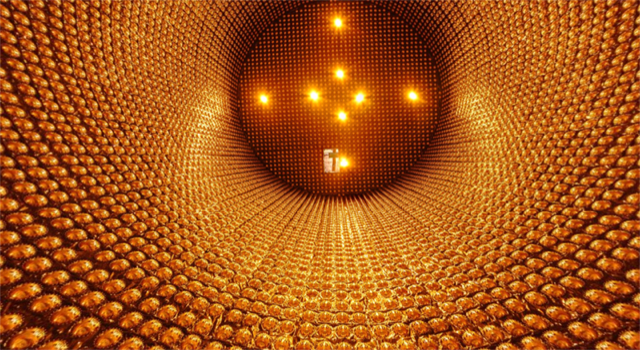
\includegraphics[width=\textwidth]{figures/kamiokande.png}}
      \vspace{1cm}

      \scalebox{0.7}{\begin{tikzpicture} \protondecay \end{tikzpicture}}
    \end{onlyenv}
    \begin{onlyenv}<1,4>
      \begin{center}
        \scalebox{0.7}{\begin{tikzpicture} \protondecay \end{tikzpicture}}
      \end{center}

    \end{onlyenv}
    \begin{onlyenv}<3>
      \begin{align*}
        P_R = \left( -1 \right)^{3 \left( B - L  \right) + 2s}
      \end{align*}
    \end{onlyenv}
    \begin{onlyenv}<1,3>
      \begin{align*}
        \begin{rcases}
          & \frac{1}{2} \lambda_{i j k }L_iL_j\bar{e}_k \\
          & \lambda'_{i j k}L_iQ_j\bar{d}_k \\
          & \mu'_iL_iH_u \\
        \end{rcases} \Delta L = 1 \\
        \begin{rcases}
          & \lambda_{i j k }'' \bar{u}_{i} \bar{d}_{j} \bar{d}_{k}
        \end{rcases} \Delta B = 1
      \end{align*}
    \end{onlyenv}
    \includegraphics<3>[width=\textwidth]{figures/rparityviolation.jpg}
  \end{column}
\end{columns}
\end{frame}

\begin{frame}<presentation:0>[noframenumbering,label=rparity]{R-parity}
  \begin{itemize}
  \item<1-> R-parity violating (RPV) models open up a largely unexplored\nocite{evans_lhc_2013}
    world of parameters and decay modes that do \textit{not} include \textcolor{red}{$\ptmiss$}.
  \item<2-> R-parity allows SUSY particles to decay to SM hadrons, resulting in a fully visible final state.
  \end{itemize}

  \begin{center}
    % \scalebox{0.7}{
    % \begin{tikzpicture}
    %   \tikzset{
    %   rpv vertex/.style={circle, inner sep=0pt, draw, minimum size=4pt, fill=red,},
    %   every blob/.style={draw=green!40!black, pattern color=green!40!black},
    % }
    %   \begin{feynman}
    %     \vertex[blob, minimum size=1cm] (base) {};
    %     \vertex[below left=1cm and 1.5cm of base] (p1) ;
    %     \vertex[above left=1cm and 1.5cm of base] (p2) ;
    %     \vertex[below right=1cm and 1.5cm of base] (stop1) ;
    %     \vertex[above right=1cm and 1.5cm of base] (stop2) ;
    %     \vertex[above right=0.3cm and 1cm of stop1] (b1) {\quarkt{}};
    %     \vertex[below right=0.3cm and 1cm of stop1] (x1) {\textcolor{red}{\neutralino{}}};
    %     \vertex[above right=0.3cm and 1cm of stop2] (b2) {\aquarkt{}};
    %     \vertex[below right=0.3cm and 1cm of stop2] (x2) {\textcolor{red}{\neutralino{}}};
    %     \begin{pgfonlayer}{back}
    %       \diagram*{
    %       (p1) -- [decorate, decoration=triple,edge label'=$P_{1}$, pos=0.] (base.center);
    %       (p2) -- [decorate, decoration=triple, edge label=$P_{2}$, pos=0.3] (base.center);
    %     };
    %       \node[draw, circle, fill=white, minimum size=1cm] {};
    %     \end{pgfonlayer} 
    %     \diagram*{
    %     (base) -- [edge label'=\stopq{}] (stop1);
    %     (base) -- [edge label=\astopq{}] (stop2);
    %     (stop1) -- [] (b1);
    %     (stop1) -- [] (x1);
    %     (stop2) -- [] (b2);
    %     (stop2) -- [] (x2);
    %   };
    %   \end{feynman}
    % \end{tikzpicture}}
    \scalebox{1}{
      \begin{tikzpicture}
        \tikzset{
          rpv vertex/.style={circle, inner sep=0pt, draw, minimum size=4pt, fill=red,},
          every blob/.style={draw=green!40!black, pattern color=green!40!black},
        }
        \begin{feynman}
          \vertex[blob, minimum size=1cm] (base) {};
          \vertex[below left=1cm and 1.5cm of base] (p1) ;
          \vertex[above left=1cm and 1.5cm of base] (p2) ;
          \vertex[below right=1cm and 1.5cm of base] (stop1) ;
          \vertex[above right=1cm and 1.5cm of base] (stop2) ;

          \vertex[above right=0.3cm and 1cm of stop1] (b1) {\quarkt{}};
          \vertex[below right=0.3cm and 1cm of stop1] (x1);

          \vertex[below right=0.3cm and 1cm of stop2] (b2) {\aquarkt{}};
          \vertex[above right=0.3cm and 1cm of stop2] (x2);

          
          \begin{onlyenv}<2>
            \vertex[below right=0.3cm and 1cm of x1] (q11) {$q$};
            \vertex[right=1cm of x1] (q12) {$q$};
            \vertex[above right=0.3cm and 1cm of x1] (q13) {$q$};
            \vertex[below right=0.3cm and 1cm of x2] (q21) {$q$};
            \vertex[right=1cm of x2] (q22) {$q$};
            \vertex[above right=0.3cm and 1cm of x2] (q23) {$q$};
          \end{onlyenv}
          \begin{pgfonlayer}{back}
            \diagram*{
              (p1) -- [decorate, decoration=triple,edge label'=$P_{1}$, pos=0.] (base.center);
              (p2) -- [decorate, decoration=triple, edge label=$P_{2}$, pos=0.3] (base.center);
            };
            \node[draw, circle, fill=white, minimum size=1cm] {};
          \end{pgfonlayer} 
          \diagram*{
            (base) -- [edge label'=\stopq{}] (stop1);
            (base) -- [edge label=\astopq{}] (stop2);
            (stop1) -- [] (b1);
            (stop1) -- [edge node={node[near end, below, color=red] {\neutralino}}] (x1);
            (stop2) -- [] (b2);
            (stop2) -- [edge node={node[near end, above, color=red] {\neutralino}}] (x2);

          };
          \begin{onlyenv}<2>
            \diagram*{
              (x1) -- (q11);
              (x1) -- (q12);
              (x1) -- (q13);
              (x2) -- (q21);
              (x2) -- (q22);
              (x2) -- (q23);

            };
          \end{onlyenv}
        \end{feynman}
      \end{tikzpicture}
    }
    % 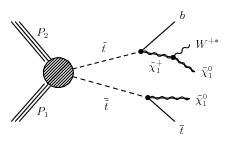
\includegraphics[width=0.5\textwidth]{figures/mssmdecay.png}
    % 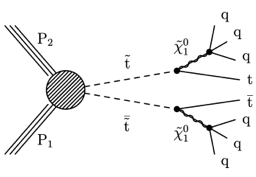
\includegraphics[width=0.5\textwidth]{figures/rpvdecay.png}
  \end{center}
\end{frame}


\newcommand{\drawdiagram}[2]{
  \tikzset{
    rpv vertex/.style={
      circle,
      inner sep=0pt,
      draw,
      minimum size=4pt,
      fill=red,
      % node contents= {},
    }
  }
  \begin{feynman}
    \vertex[] (base);
    \vertex[left=of base, rpv vertex] (stop) {};
    \vertex[above left =of stop] (q1) {#1};
    \vertex[below left =of stop] (q2) {#2};
    \vertex[above right=of base] (stopb) {\aquarkb} ;
    \vertex[below right=of base] (a2);
    \vertex[above right=of a2] (xb) {\quarkb};

    \vertex[below right=of a2, rpv vertex] (a3) {};
    \vertex[below right=of a3] (xs) {#1};
    \vertex[above right=of a3] (xd) {#2};
    \diagram*{
      (q1) -- [] (stop);
      (q1) -- [] (stop);
      (q2) -- [] (stop);
      (stop) -- [edge label=\stopq] (base);
      (base) -- [] (stopb);
      (base) -- [ edge label'=\chargino] (a2);
      (a2) -- [ edge label'=\vstopq] (a3);
      (a2) -- [] (xb);
      (a3) -- [] (xs);
      (a3) -- [] (xd);
    };
  \end{feynman}

}


\begin{frame}{Single \stopq{} Production}
  \begin{itemize}
  \item We focus our efforts on the $\lambda_{3jk}''$  terms, which allows a \stopq{} to couple to SM quarks.
  \item The decay we focus on involved the production of a \stopq{} through the  $\lambda_{3jk}''$ coupling, then the decay to a fully hadronic state.
  \end{itemize}
  \begin{center}
    \begin{tikzpicture}
      \drawdiagram{$d_{i}$}{$d_{j}$}
      \node (X) at (-1,-2) {RPV Vertex};
      \draw[->] (X) -- (stop);
      \draw[->] (X) -- (a3);
    \end{tikzpicture}
  \end{center}
\end{frame}

\section[Signal Phenomenology]{Single $\stopq$ Signal Phenomenology}
\label{sec:signal}

\newenvironment{greenenv}{\only{\setbeamercolor{local structure}{fg=green}}}{}
\newenvironment{blueenv}{\only{\setbeamercolor{local structure}{fg=blue}}}{}
\newenvironment{redenv}{\only{\setbeamercolor{local structure}{fg=red}}}{}

\begin{frame}{Process Regimes}

  % \begin{onlyenv}<1>
  %   \begin{itemize}
  %   \item Different coupling strengths and sparticle masses results in different decay geometries. 
  %   \item We need to identify the parameter spaces that are both unexplored and experimentally accessible. 
  %   \end{itemize}
  % \end{onlyenv}

  % \begin{onlyenv}<1>
  %   \begin{center}
  %     \begin{tikzpicture}
  %       \node[draw, minimum size=2cm, align=center, circle ] (A) at (-3,0) {Coupling};
  %       \node[draw, minimum size=2cm, align=center, circle ] (B) at (0,0) {$m_{\stopq}$};
  %       \node[draw, minimum size=2cm, align=center, circle ] (C) at (3,0) {$m_{\chargino}$};
  %     \end{tikzpicture}
  %   \end{center}    
  % \end{onlyenv}


  \definecolor{dijetblue}{HTML}{647FB3} % 0,32,250
  \definecolor{longlived}{HTML}{9083B8} % 0,32,250
  \definecolor{ssyellow}{HTML}{D8A036} % 0,32,250
  \definecolor{myred}{rgb}{.7,.1,.1}
  \begin{onlyenv}<1>
    \begin{block}{Coupling}
      \begin{itemize}
      \item<red@1-> Weak coupling ($ \approx \lambda < 0.1$): the produced stop is long lived.
      \item<blue@1-> Strong coupling ($ \approx \lambda > 0.4$): the produced stop decays promptly back to quarks, resulting in dijets.
      \item<green@1-> The intermediate regime is an unexplored territory. 
      \end{itemize}
      \begin{center}
        \begin{center}
          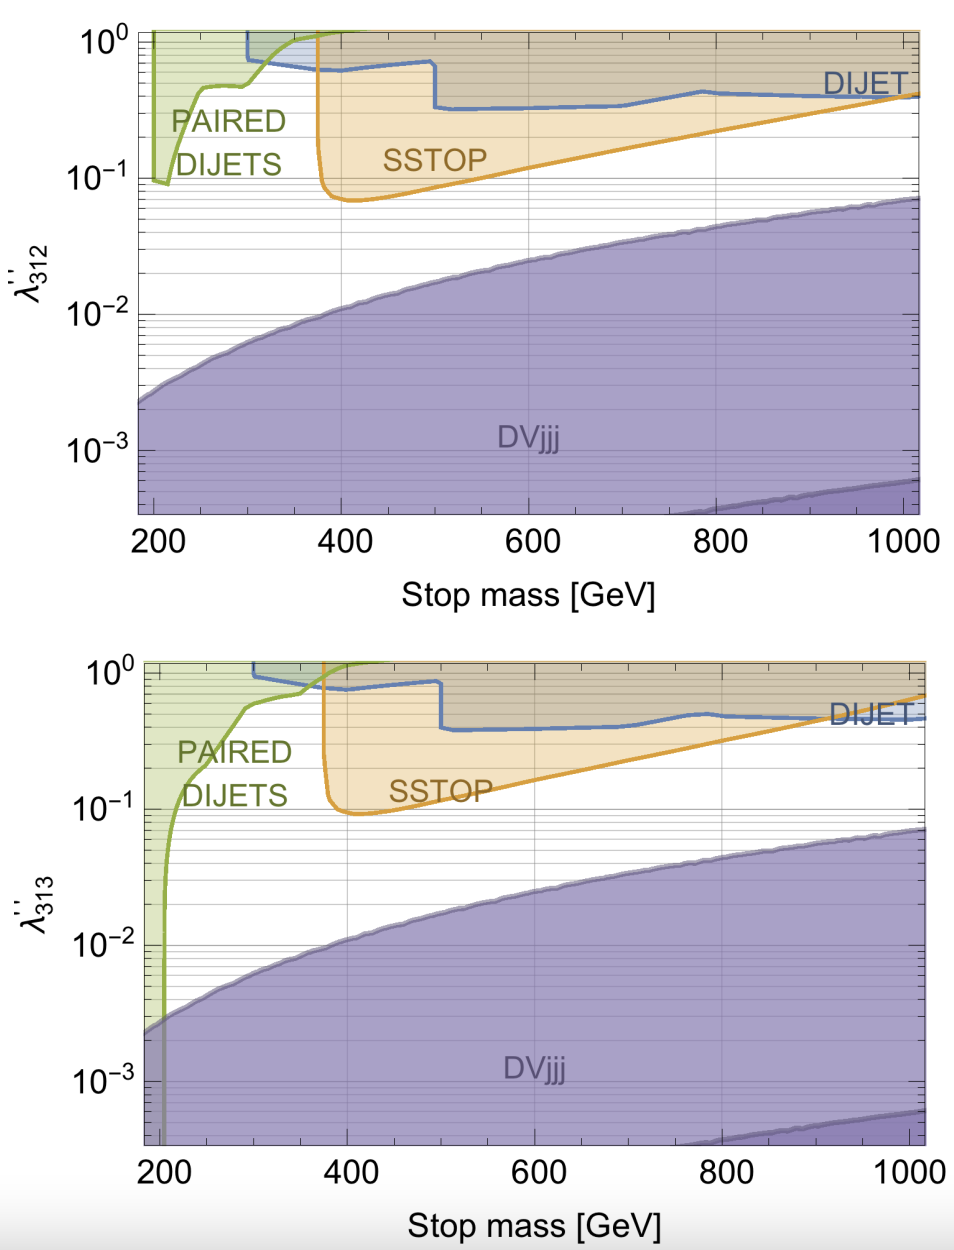
\includegraphics[trim={0 11cm 0 0}, clip, width=0.4\textwidth]{figures/paramspace.png}
        \end{center}
        \begin{tikzpicture}
          \draw[->] (0,0) -- (6,0) node [at end, right] {$\lambda_{3jk}''$} node[at start, left] {0};
          \draw[] (0,-0.05) -- (0,0.05);
          \draw[very thick, draw=longlived, fill=longlived, fill opacity=0.2] (1,0) ellipse ( 1 and 0.2);
          \draw[] (2,-0.05) -- (2,0.05) node[at start, below] {$0.1$};
          \draw[very thick] (3,0) ellipse ( 1 and 0.2);
          \draw[] (4,-0.05) -- (4,0.05) node[at start, below] {$0.4$};
          \draw[very thick, draw=dijetblue, fill=dijetblue, fill opacity=0.2] (5,0) ellipse ( 1 and 0.2);
        \end{tikzpicture}
      \end{center}
    \end{block}
  \end{onlyenv}

  \begin{onlyenv}<2>
    \begin{block}{Mass Regimes}
      \begin{columns}
        \begin{column}{0.4\textwidth}

          \begin{center}
            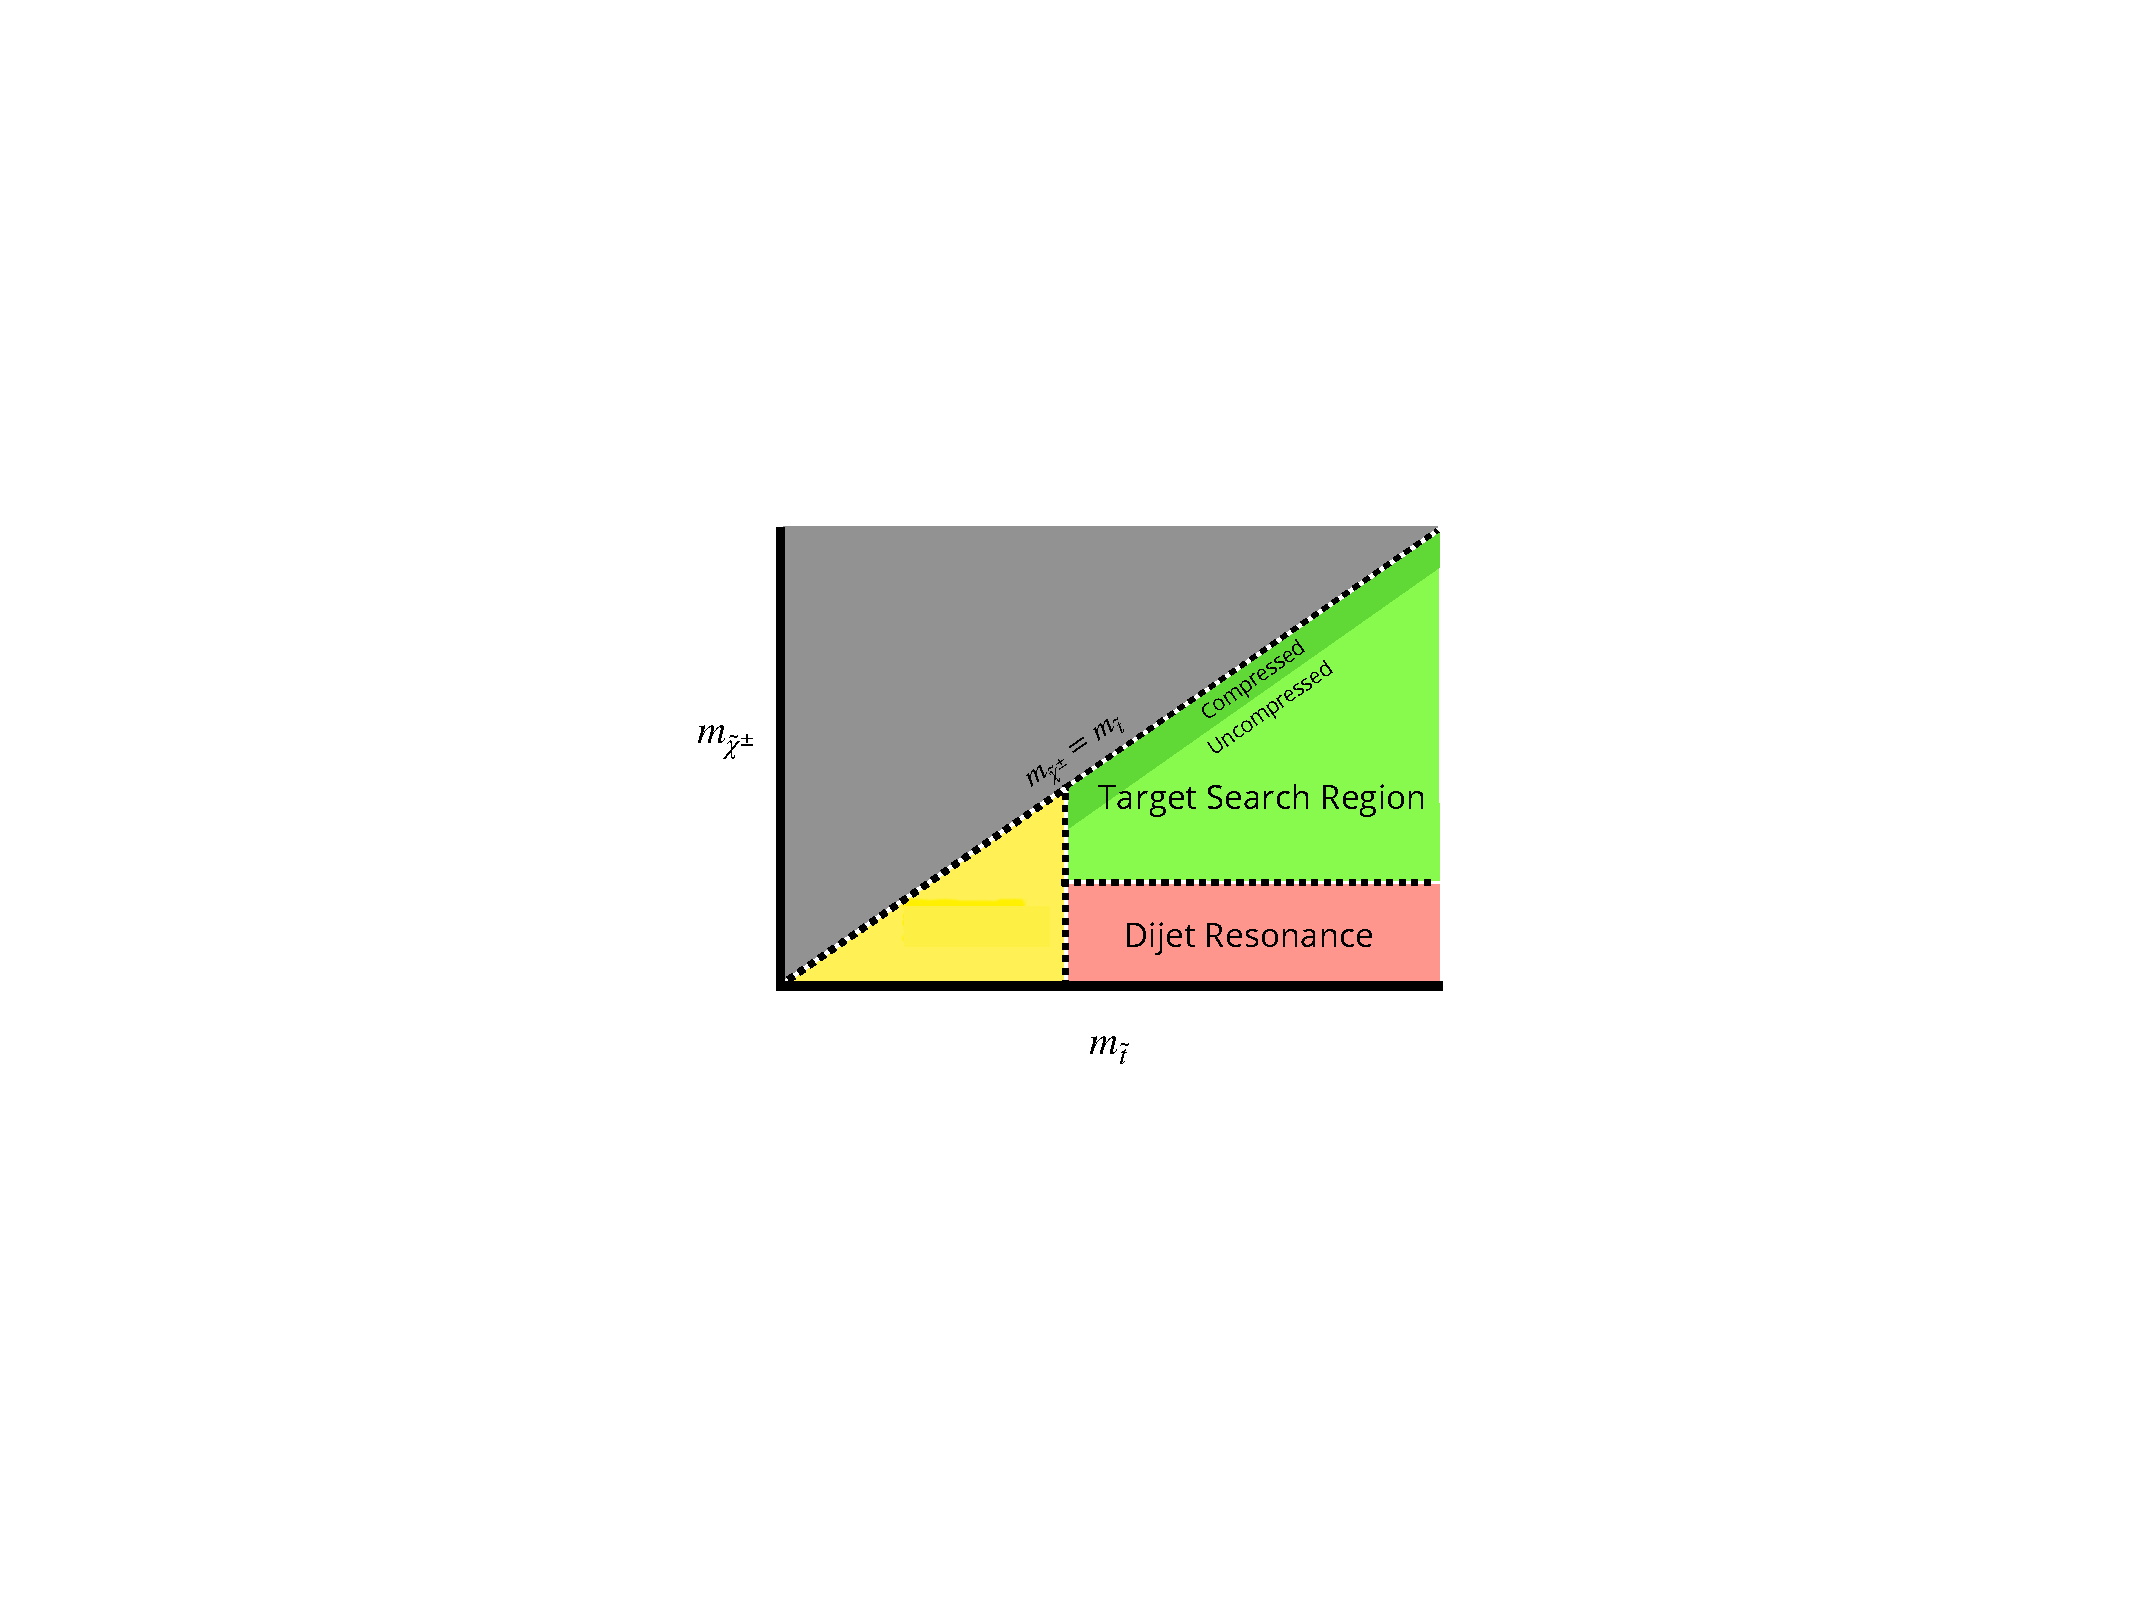
\includegraphics[width=\textwidth]{figures/ParameterSpaceCartoonUpdated.pdf}
          \end{center}
          \par

          \begin{center}
            \begin{tikzpicture}[scale=0.5]
              \def\N{5}
              % \foreach \i [evaluate={\y=\i-0.5; \Nx=\N-\i+1; \e=0.5*\i}] in {1,...,\N}{
              % \draw[very thin,dashed,black!50] (0,\i) --++ (\Nx,0);
              % \draw[very thin,dashed,black!50] (\i,0) --++ (0,\Nx);
              % \tick{0,\i}{0} node[left=-1,scale=0.9] {\e};
              % \tick{\i,0}{90} node[below=-1,scale=0.9] {\e};
              % }
              \foreach \i/\conecolbase [evaluate={\y=\i-0.5; \Nx=\N-\i+1; \e=0.5*\i}] in {1/blue}{
                \foreach \j [evaluate={\x=\j-0.5; \mix=100-60*(\j-1)/(\N-1);
                  \ang=60*(\i-1)/(\N-1); % seperation
                  \dang=90-60*(\j-1)/(\N-1); % boost
                }] in {1,...,\Nx}{
                  \colorlet{conecol}{\conecolbase!\mix} % color for cone
                  \coordinate (O) at (\x,\y); % primary vertex
                  \coordinate (T) at ($(\x,\y)+(\ang+\dang:0.42)$); % top jet
                  \coordinate (B) at ($(\x,\y)+(\ang-\dang:0.42)$); % bottom jet
                  \jetcone[conecol]{O}{T}{30}{0.06} %!70!white
                  \jetcone[conecol]{O}{B}{30}{0.16}
                }
              }

              \draw[->] (0,-0.1)  -- (1.1*\N,-0.1) node[below, pos=0.5, align=center] {Increasing Boost ($p_{T}$)\\ Merges Jets};
              % \draw[<->,thick] (0,1.1*\N) node[left=12,above right=-3] {$\frac{1}{2}\Delta\eta = \frac{1}{2}|\eta_1-\eta_2|$} --
              % (0,0) -- (1.1*\N,0) node[yshift=-10pt,below left=0pt] {Boost $\frac{1}{2}|\eta_1+\eta_2|$}; %\eta_\text{b} = 
              % \begin{scope}[shift={(4,4)},scale=1.2]
              %   \coordinate (O) at (0,0); % primary vertex
              %   \coordinate (T) at (130:0.66); % muons
              %   \coordinate (B) at (-40:0.66); % jet cone
              %   \draw[dashed,very thin] (0,-0.7) -- (0,0.7);
              %   \draw[myorange!60!yellow!90,thick] (-0.65,0) -- (0.65,0)
              %   node[above=1,right,scale=1,align=left] {beam\\[-2pt]axis};
              %   \jetcone[blue]{O}{T}{25}{0.16}
              %   \jetcone[blue]{O}{B}{25}{0.16}
              % \end{scope}
            \end{tikzpicture}
          \end{center}
        \end{column}
        \begin{column}{0.6\textwidth}
          \begin{itemize}
          \item Low $m_{\stopq}$ lies below the ``standard'' triggers.
          \item When $m_{\chargino} \ll m_{\stopq}$ the \chargino daughters are merged, making the topology look like dijets, a very well studied model.
          \item The remaining region is unexplored.
          \end{itemize}
        \end{column}
      \end{columns}
    \end{block}
  \end{onlyenv}

  \begin{onlyenv}<3>
    \begin{block}{Compressed and Uncompressed Categories}
      \begin{columns}
        \begin{column}{0.4\textwidth}
          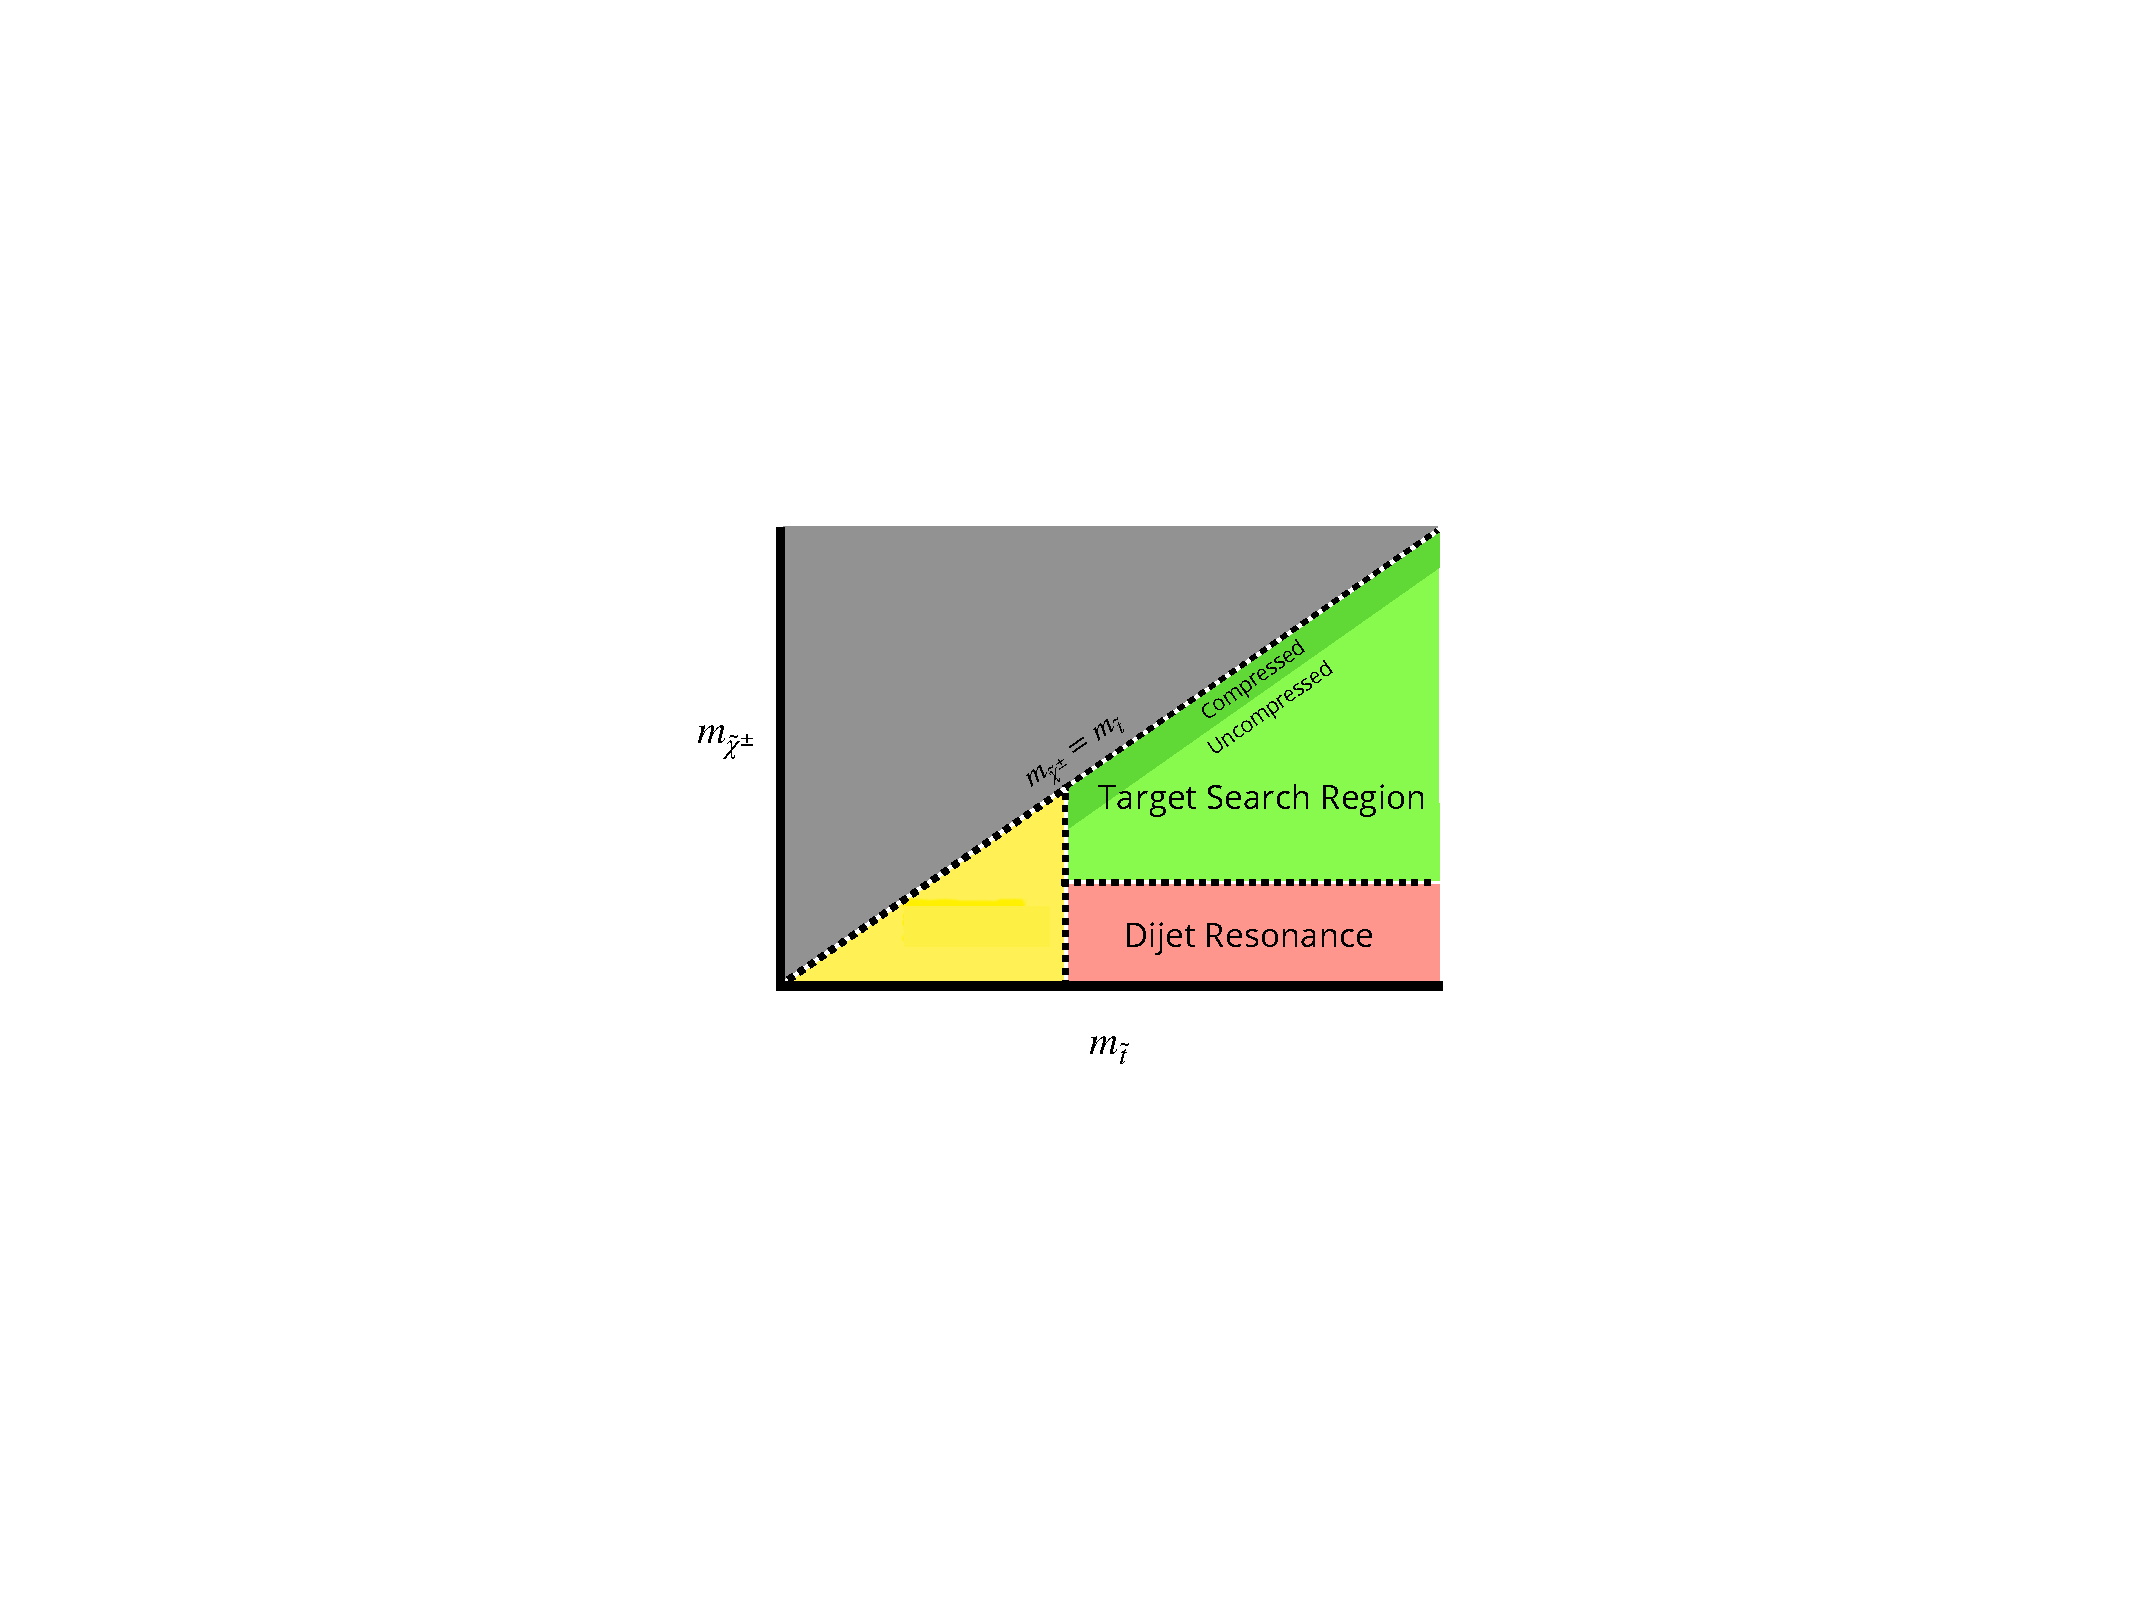
\includegraphics[width=\textwidth]{figures/ParameterSpaceCartoonUpdated.pdf}
        \end{column}
        \begin{column}{0.6\textwidth}
          Within this unexplored space, distinct geometries emerge 
          \begin{itemize}
          \item When $m_{\chargino}$ is close to $m_{\stopq}$ we say the point is compressed
          \item Otherwise we say the point is uncompressed.
          \end{itemize}
        \end{column}
      \end{columns}
    \end{block}
  \end{onlyenv}
\end{frame}


\begin{frame}{Target Signal Regime}
  \begin{columns}
    \begin{column}{0.5\textwidth}
      \begin{itemize}
      \item Target both $\lambda_{312}''$ and $\lambda_{313}''$, both of which have a good balance of cross section and b-tagging (identifying if a jet originated from a \quarkb).
      \item<only@2> For both couplings, target $0.1 < \lambda_{3jk} '' < 0.4$.
      \item<only@2> Examine both the compressed and uncompressed category.
      \item<only@2> \textbf{Perform studies on conservative $\lambda_{312}'' = 0.1$}.
      \end{itemize}

      \begin{onlyenv}<1>
        \vspace{1cm}
        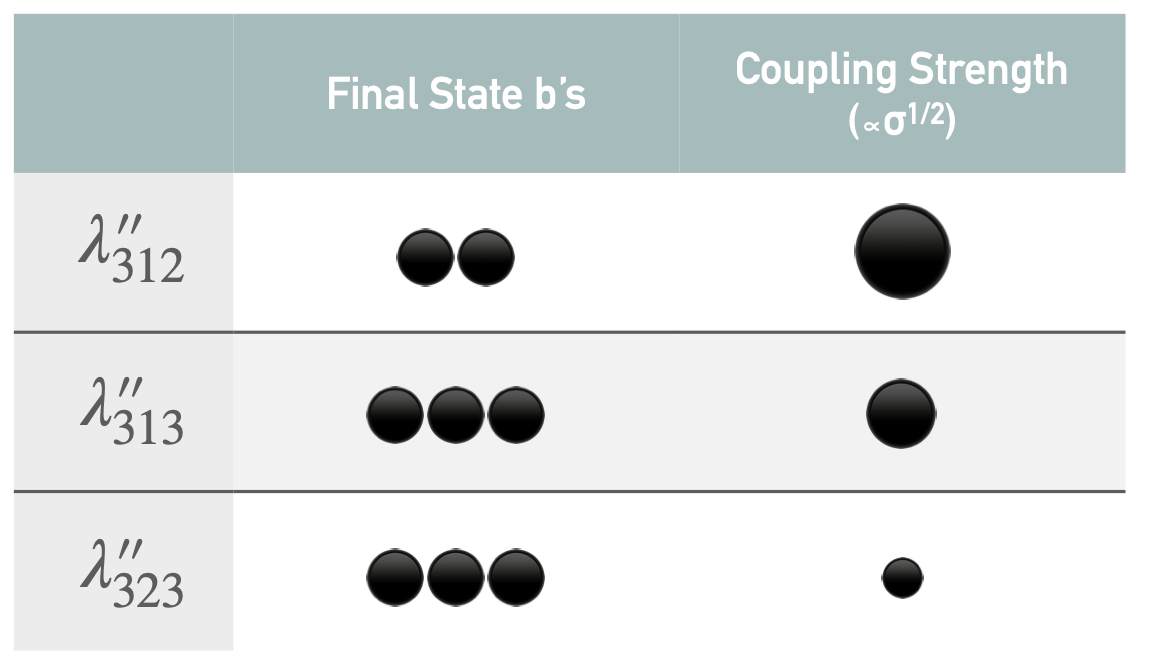
\includegraphics[width=1\textwidth]{figures/btable.png}
      \end{onlyenv}
    \end{column}
    \begin{column}{0.4\textwidth}
      \begin{center}
        \scalebox{0.5}{
          \begin{tikzpicture}
            \drawdiagram{\quarks /\quarkb}{\quarkd}
          \end{tikzpicture}
        }

        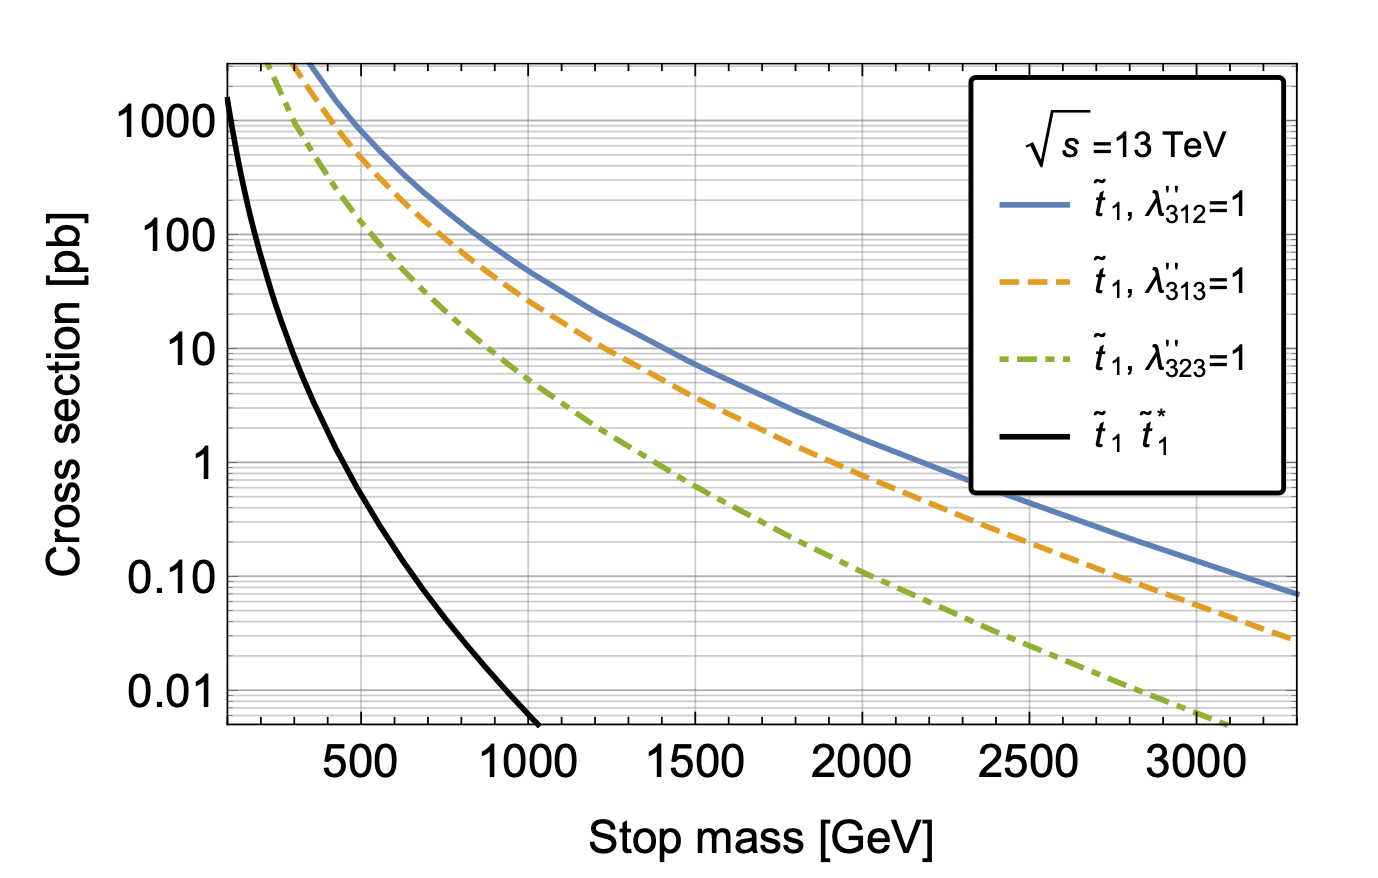
\includegraphics[width=1\textwidth]{figures/xsec.png}
      \end{center}
    \end{column}
  \end{columns}
\end{frame}


\newcommand<>\hlbox[2]{\alt#3{\frame{#2}}{#2}}

\begin{frame}<3,5>[noframenumbering, label=galleryslide]{Signal Geometry}
  %\begin{onlyenv}<1>
  %  \begin{itemize}
  %  \item The relative simplicity of this signal makes kinematic analysis more intuitive compared to high jet multiplicity analyses. 
  %  \item We can understand the event shape using generator level quantities.
  %  \end{itemize}
  %\end{onlyenv}
%  \begin{center}
    %\begin{onlyenv}<1>
      %\hyperlink{galleryslide<2>}{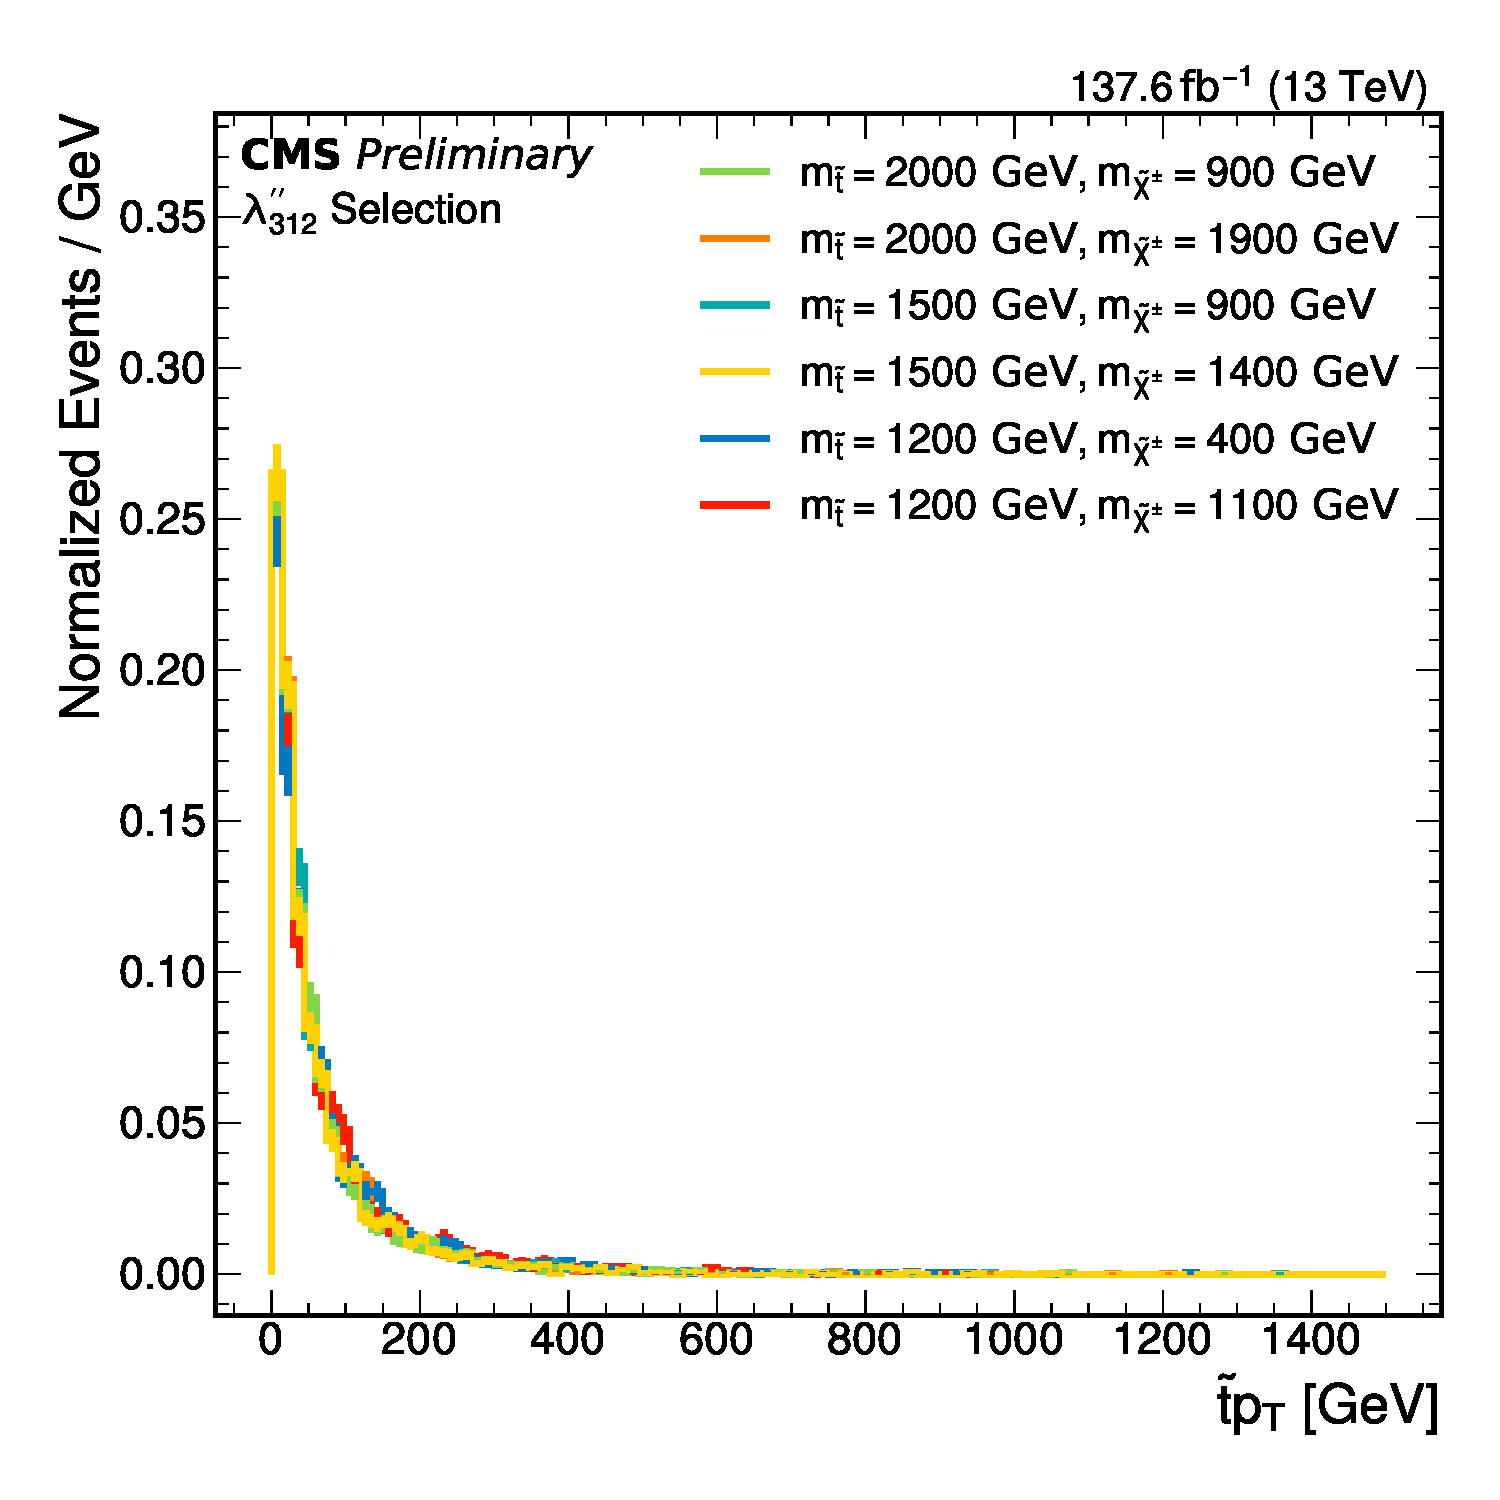
\includegraphics[width=0.24\textwidth]{figures/stop_pt.pdf}}
      %\hyperlink{galleryslide<3>}{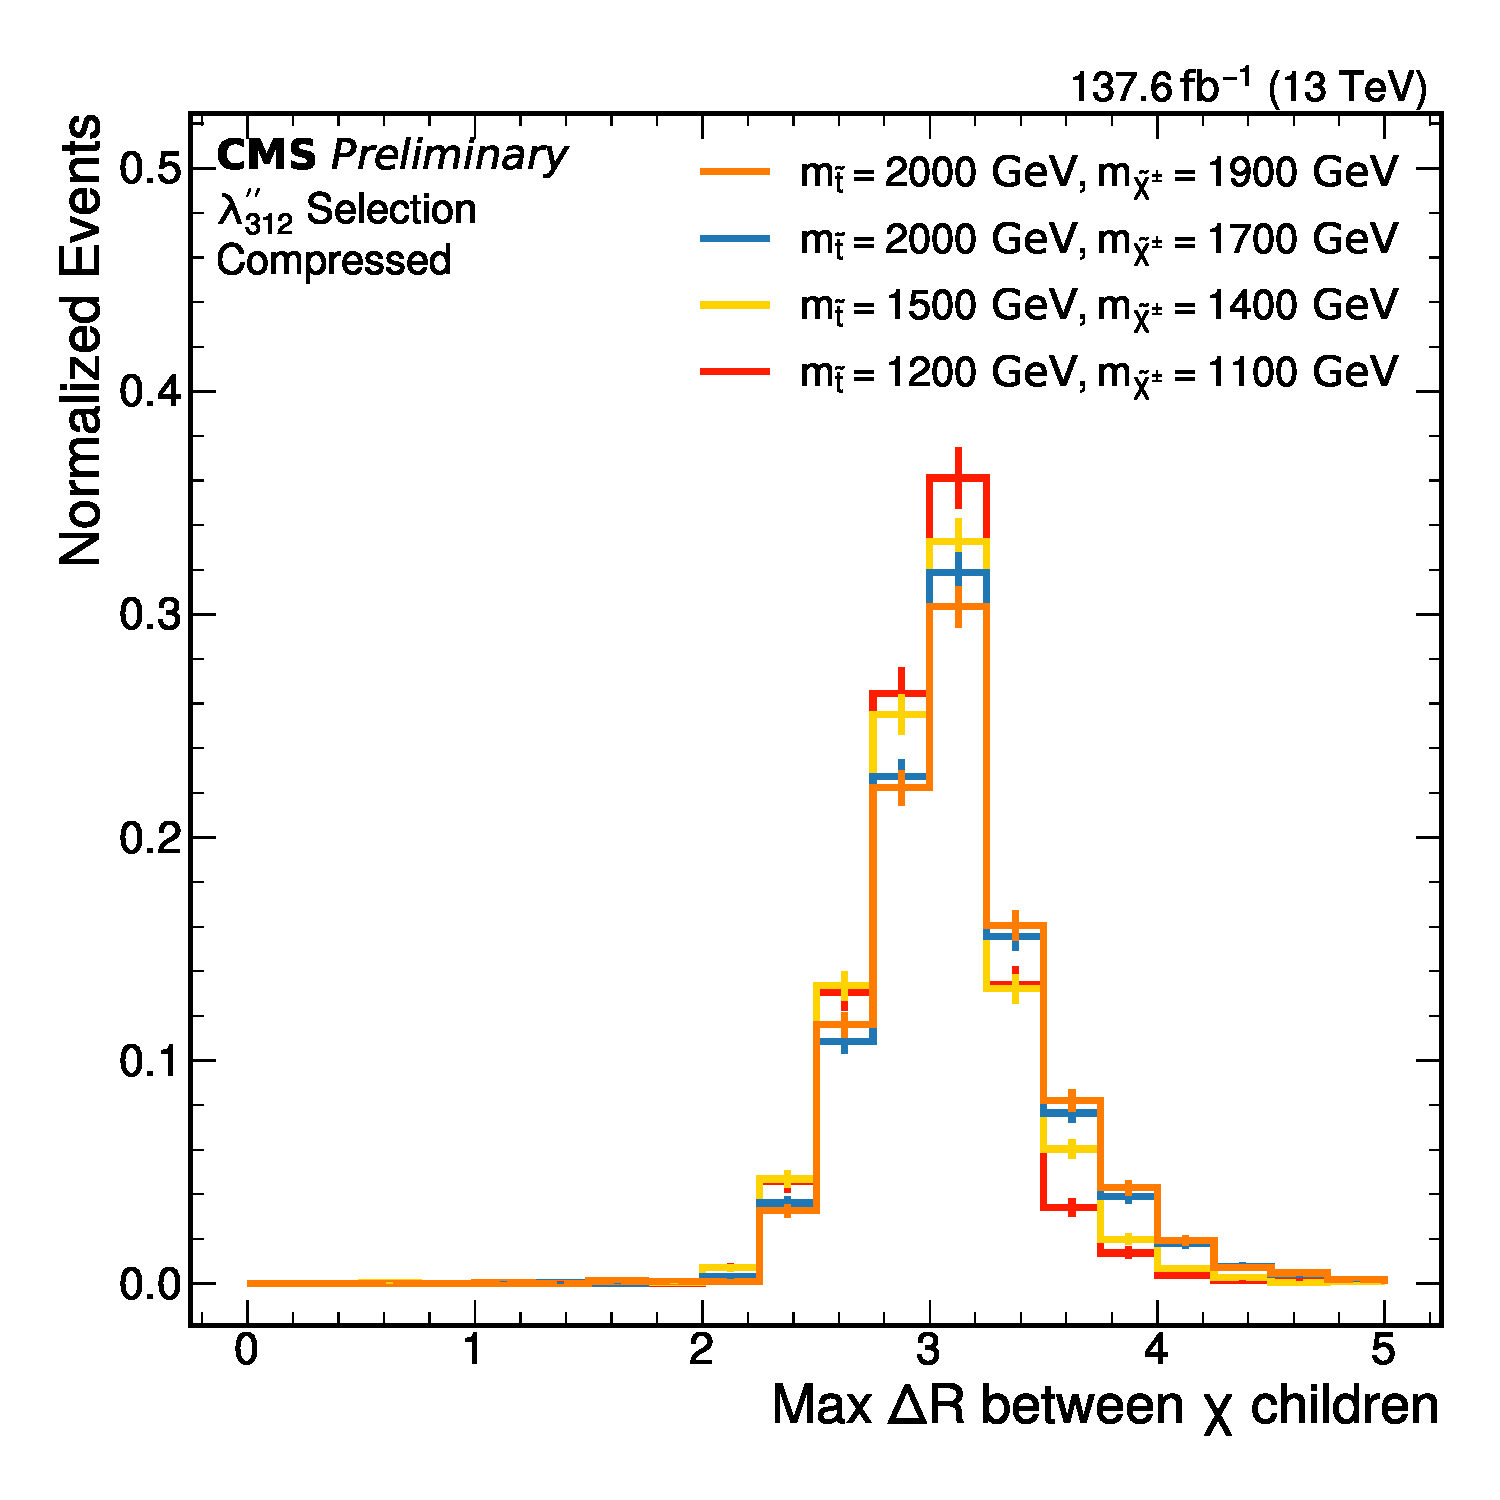
\includegraphics[width=0.24\textwidth]{figures/compressed_max_chi_child_dr.pdf} }
      %\hyperlink{galleryslide<3>}{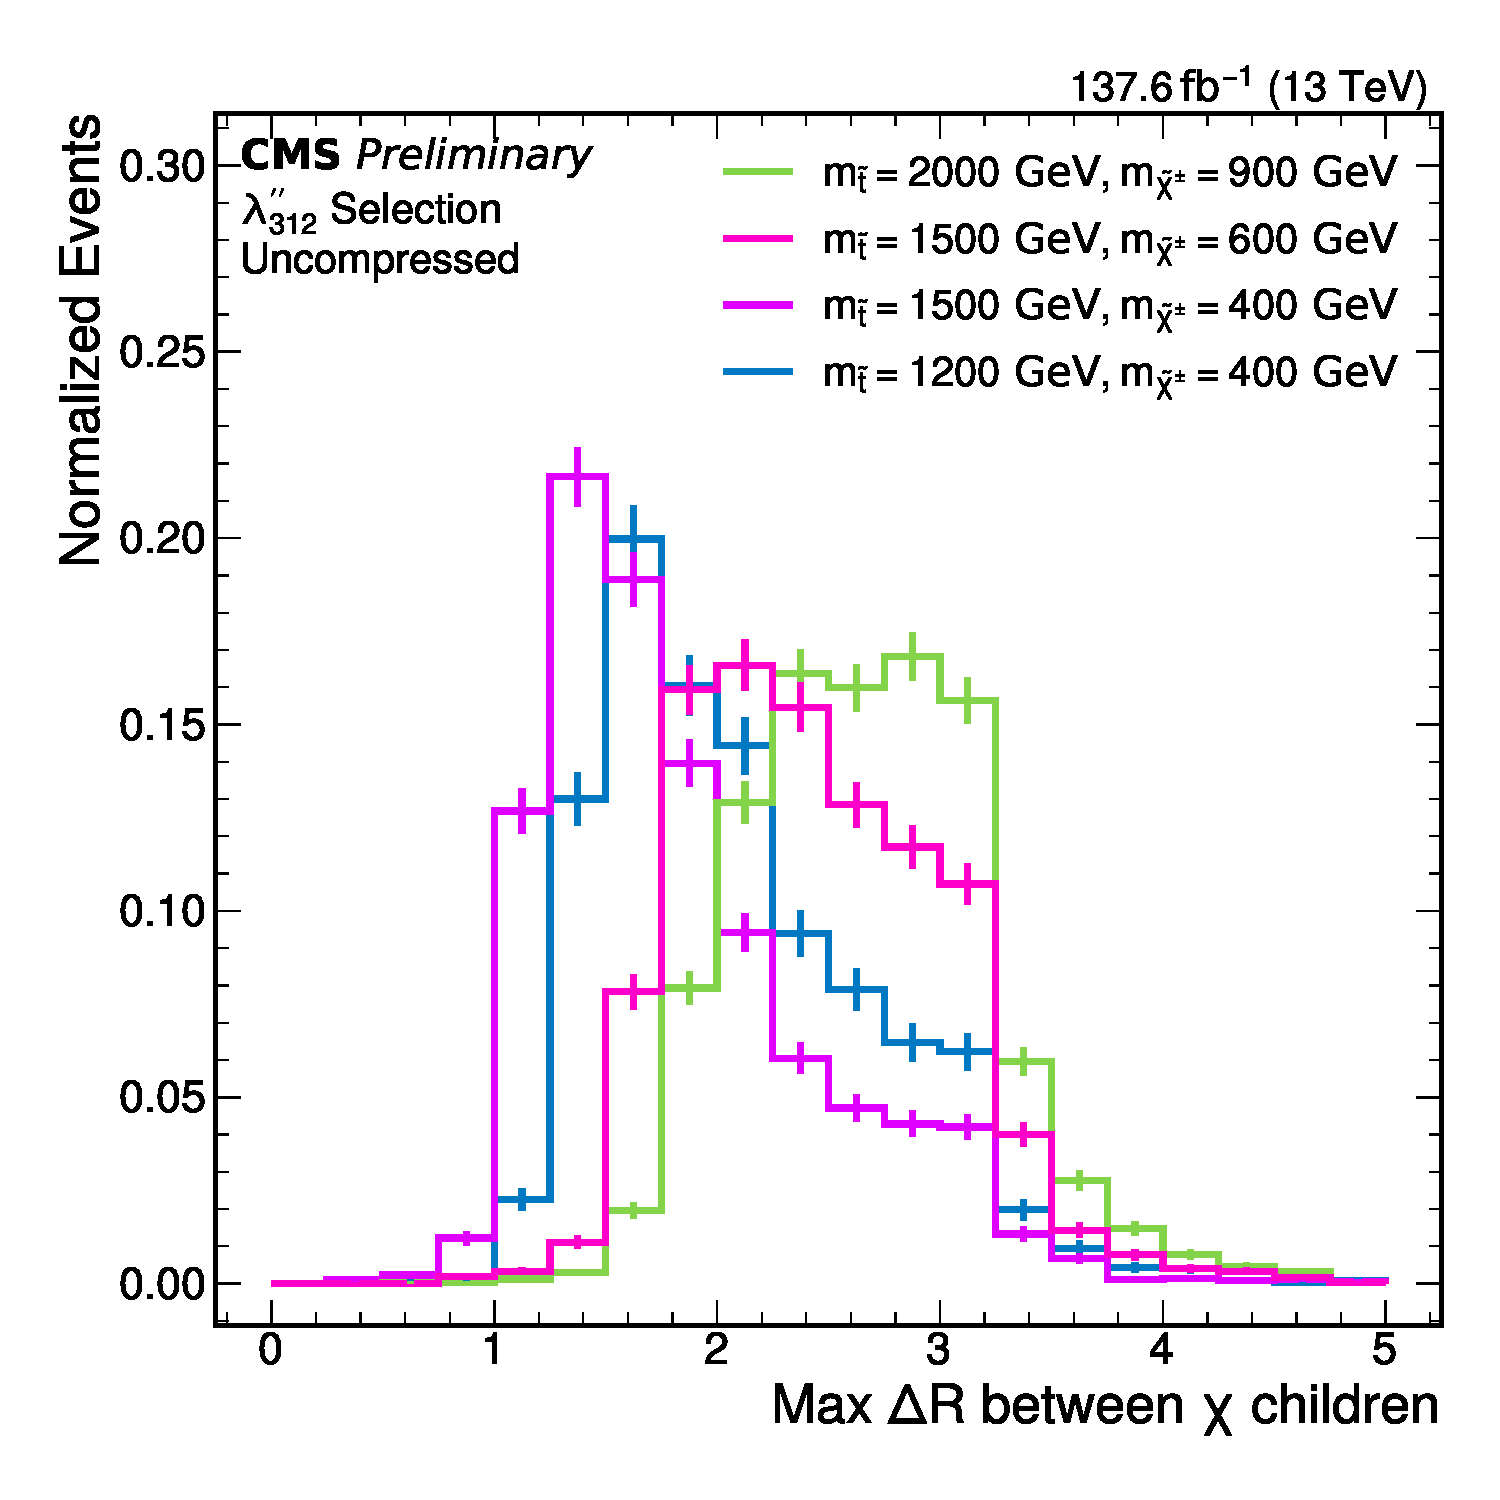
\includegraphics[width=0.24\textwidth]{figures/uncompressed_max_chi_child_dr.pdf} }
      %\hyperlink{galleryslide<4>}{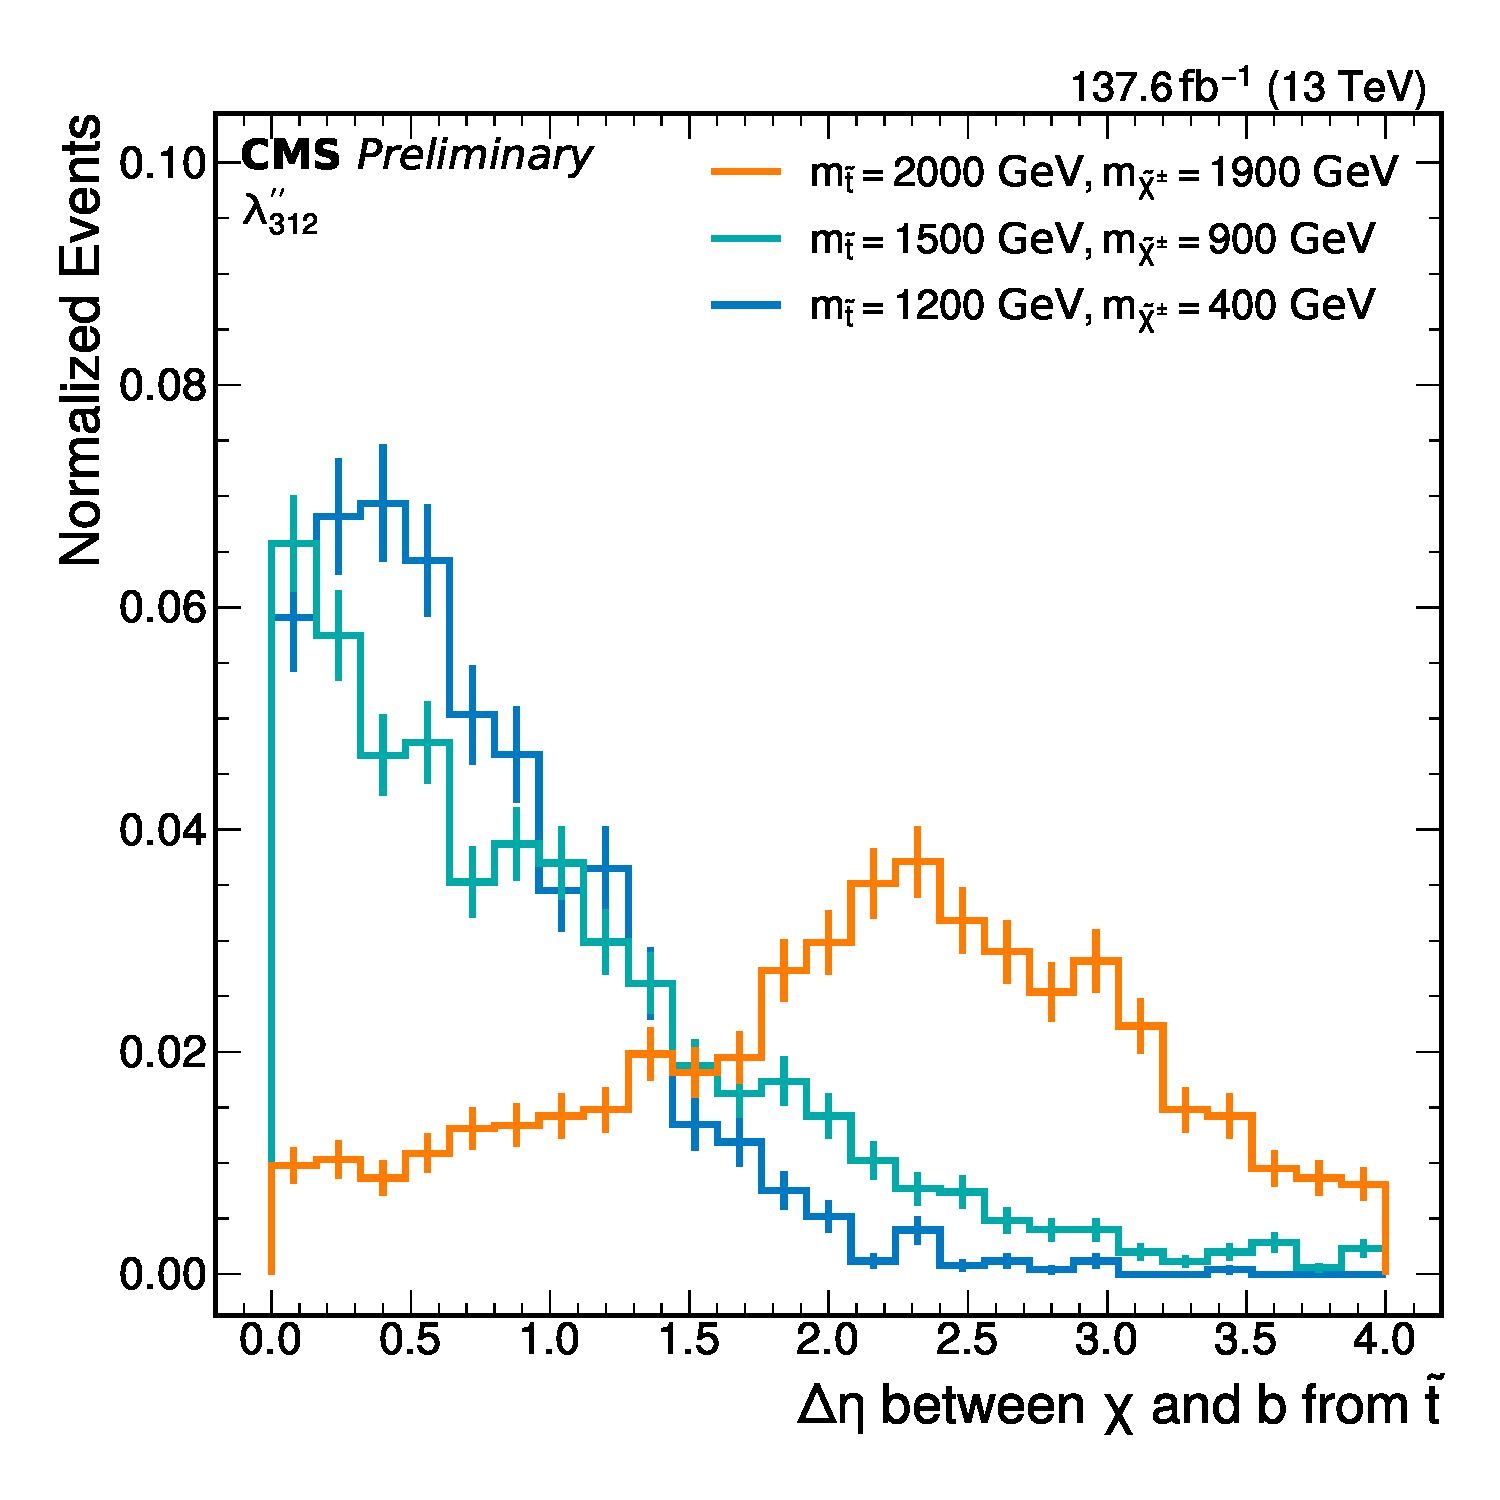
\includegraphics[width=0.24\textwidth]{figures/chi_b_eta.pdf} }
      %\hyperlink{galleryslide<4>}{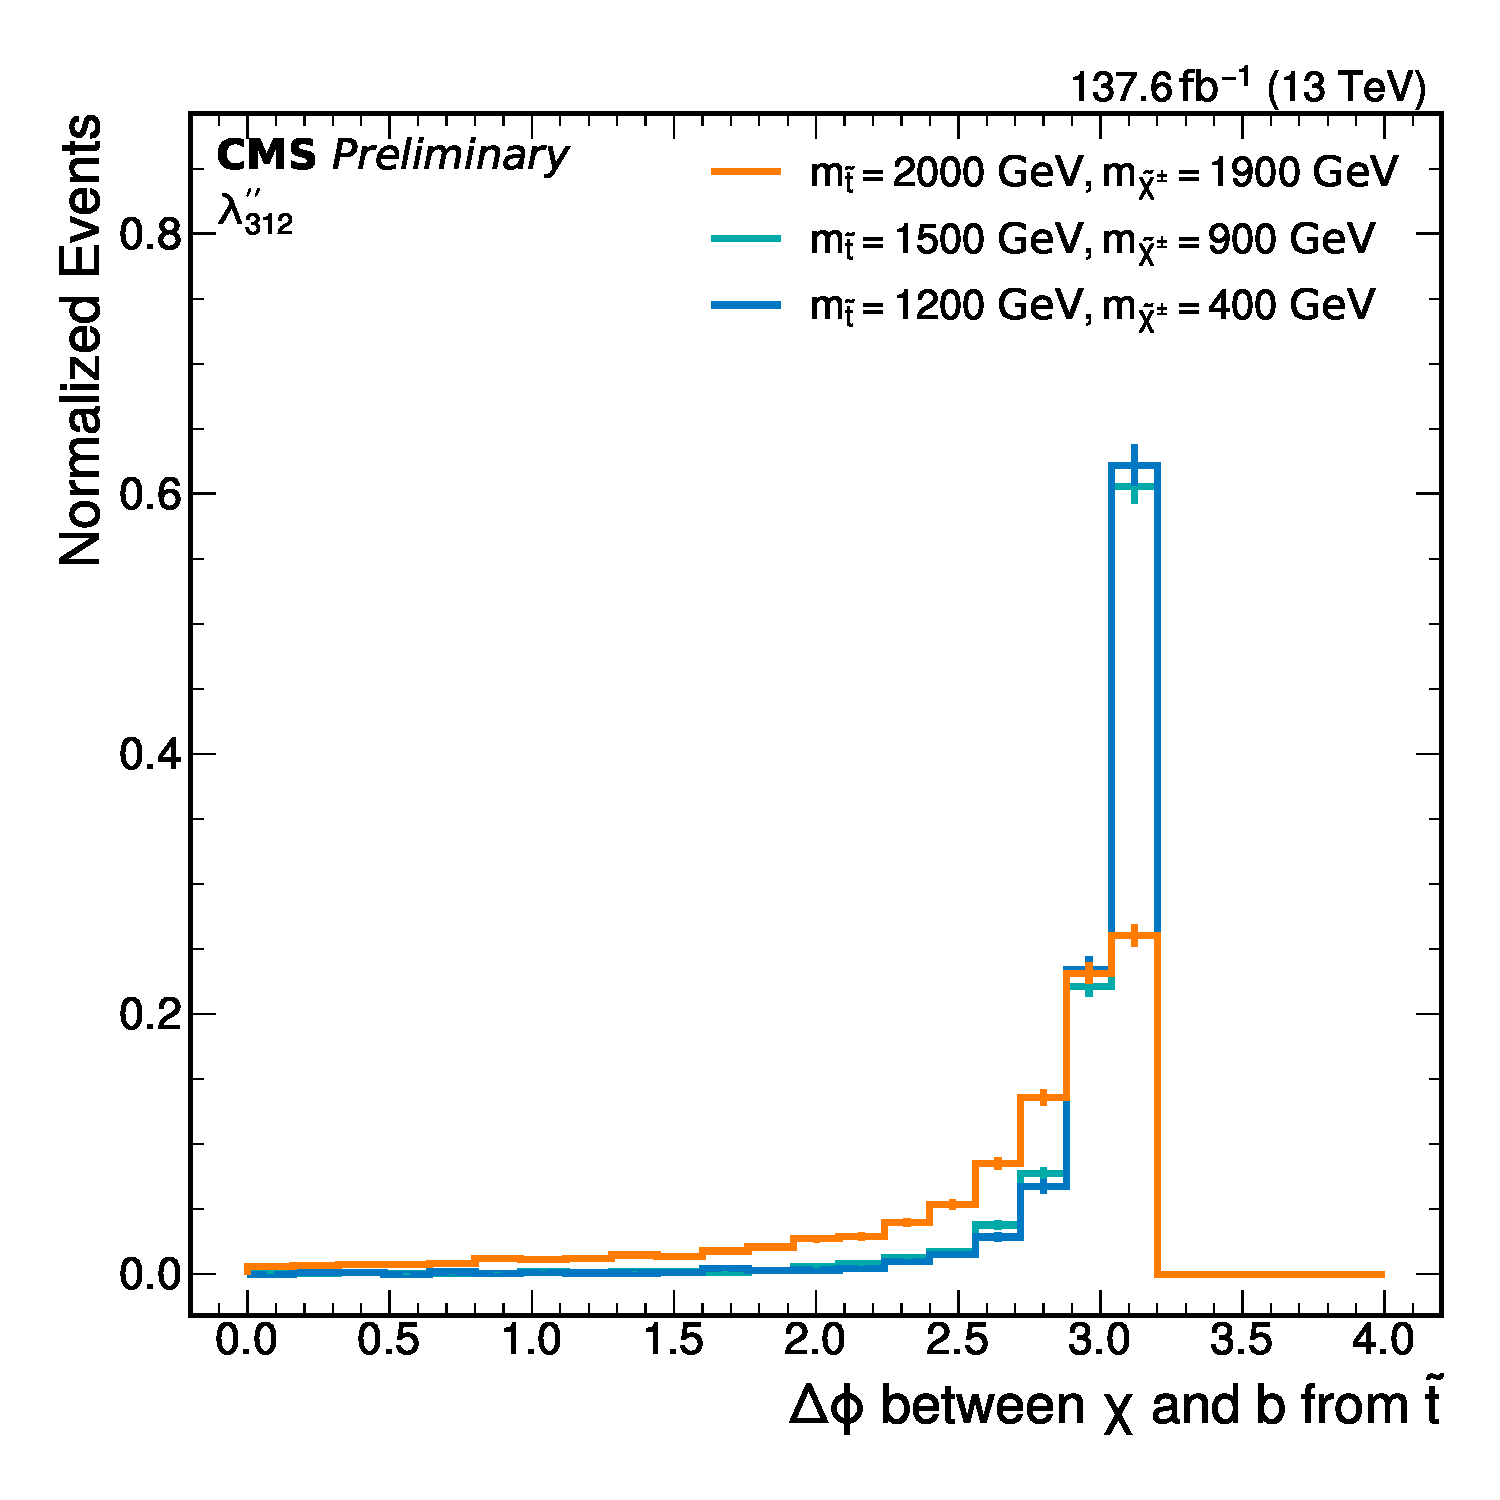
\includegraphics[width=0.24\textwidth]{figures/chi_b_phi.pdf} }
      %\hyperlink{galleryslide<4>}{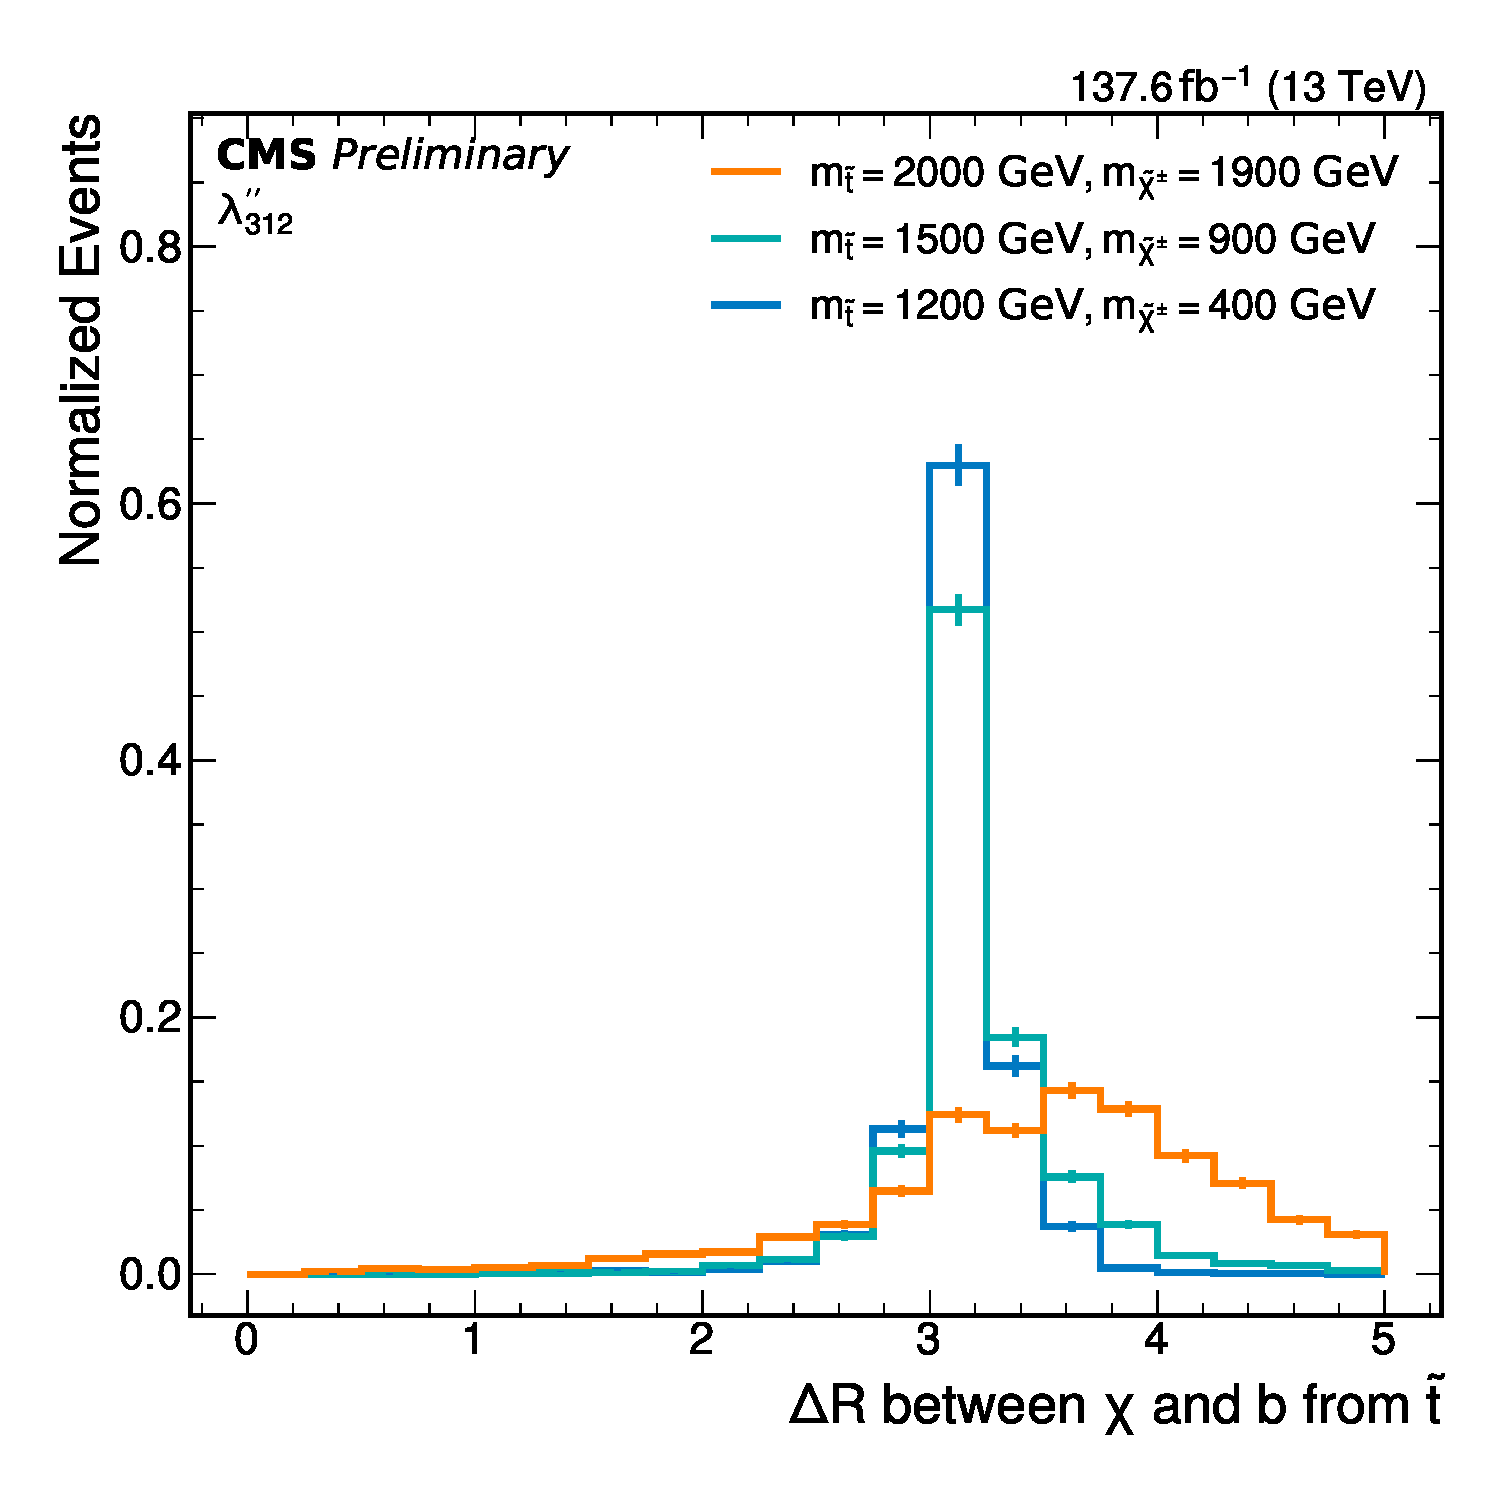
\includegraphics[width=0.24\textwidth]{figures/chi_b_dr.pdf} }
      %\hyperlink{galleryslide<5>}{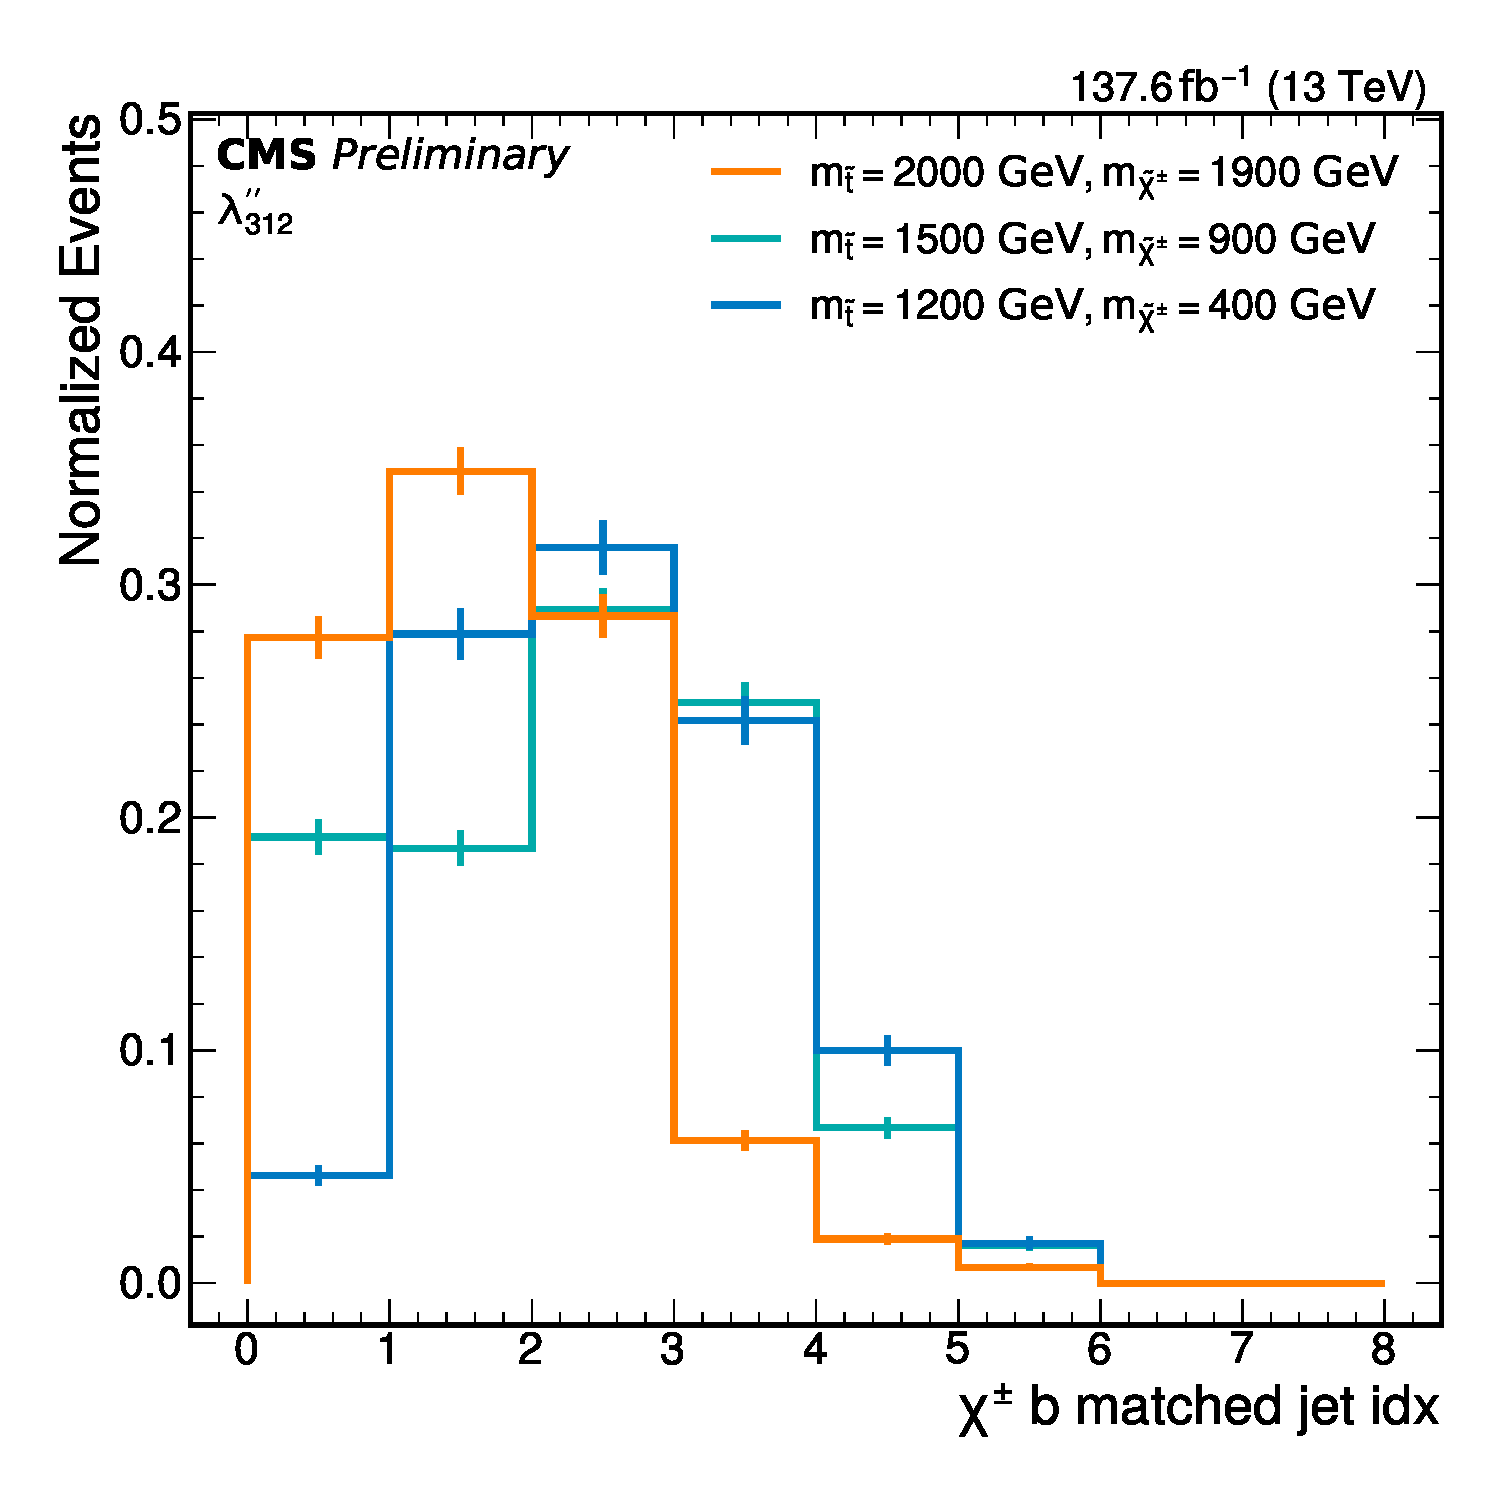
\includegraphics[width=0.24\textwidth]{figures/chi_b_jet_idx.pdf} }
      %\hyperlink{galleryslide<5>}{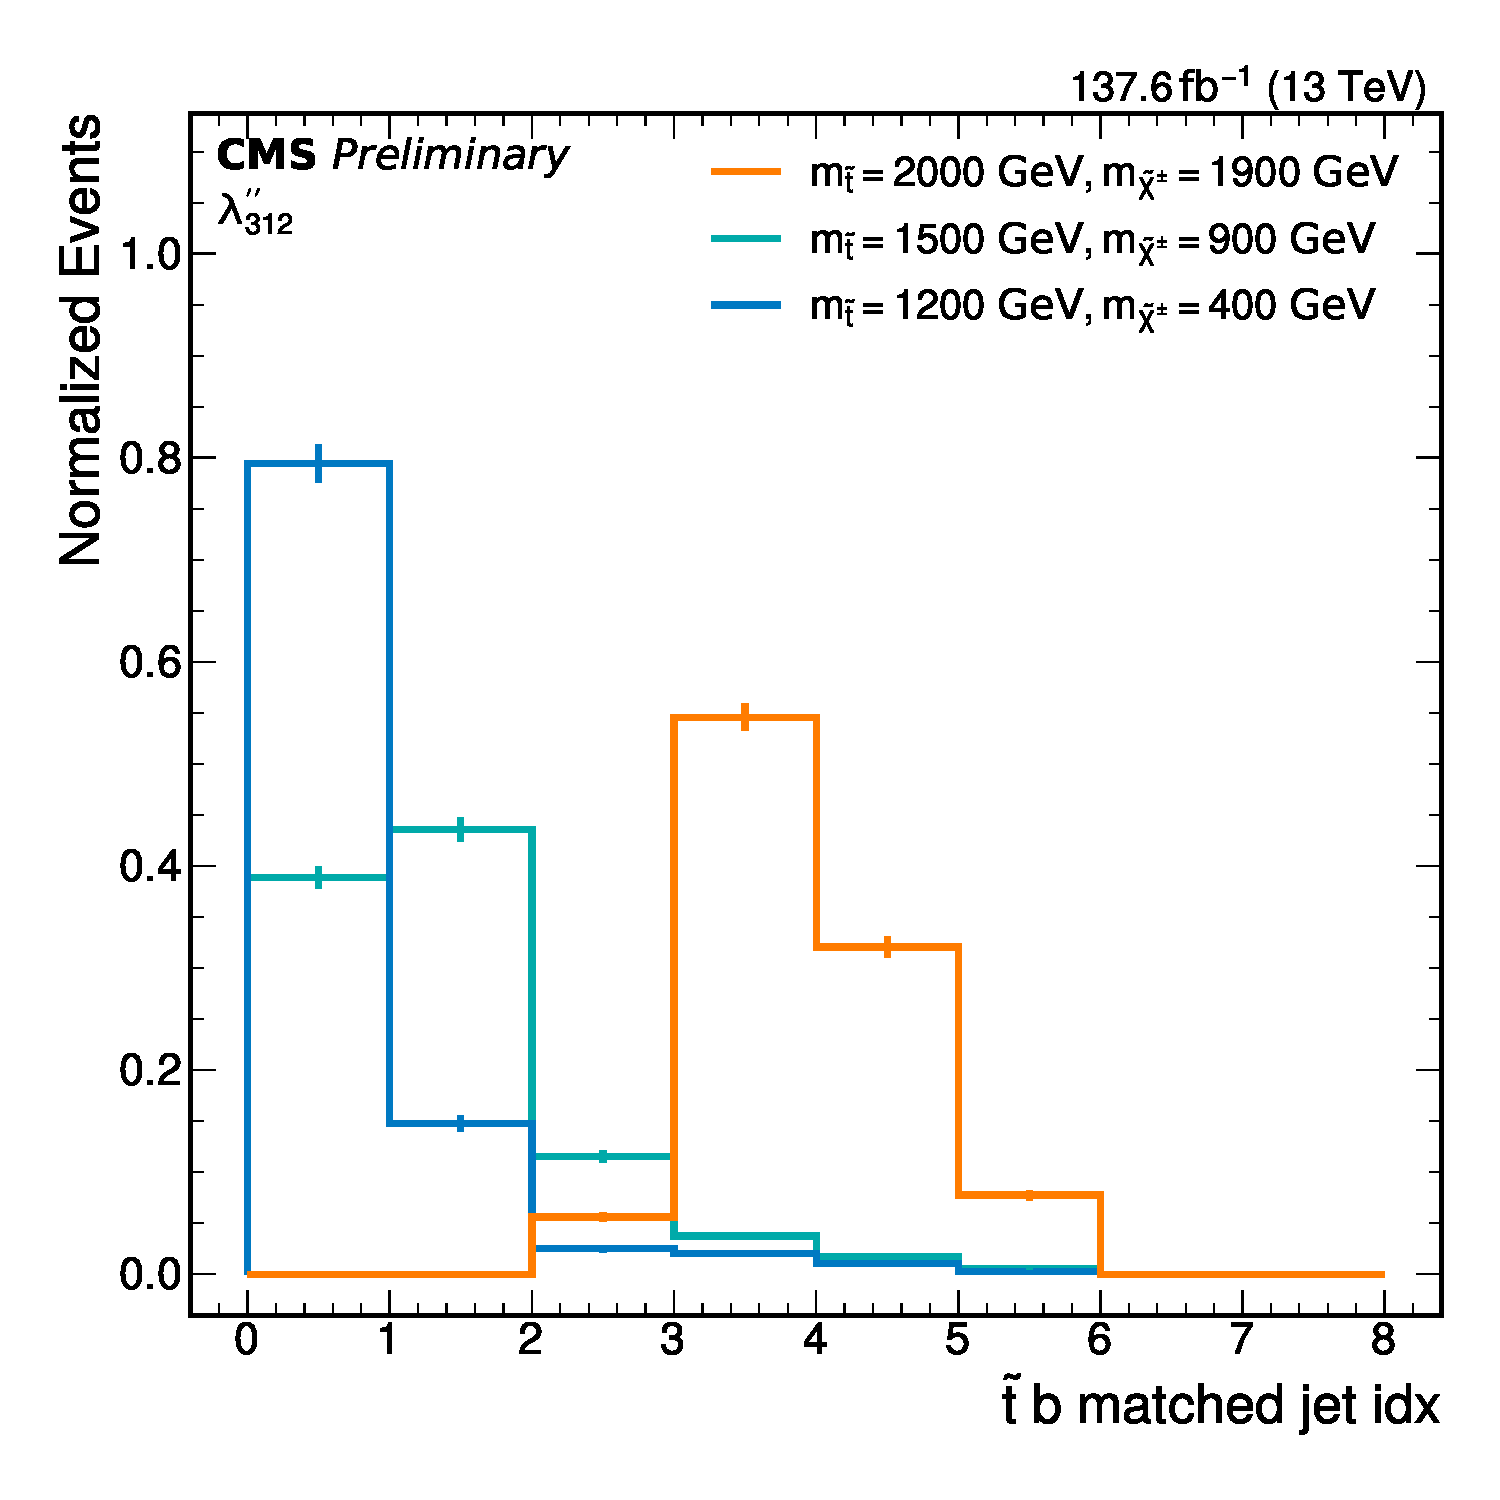
\includegraphics[width=0.24\textwidth]{figures/stop_b_jet_idx.pdf} }
    %\end{onlyenv}
    %\begin{onlyenv}<2->
      %\hlbox<2>{red}{\hyperlink{galleryslide<2>}{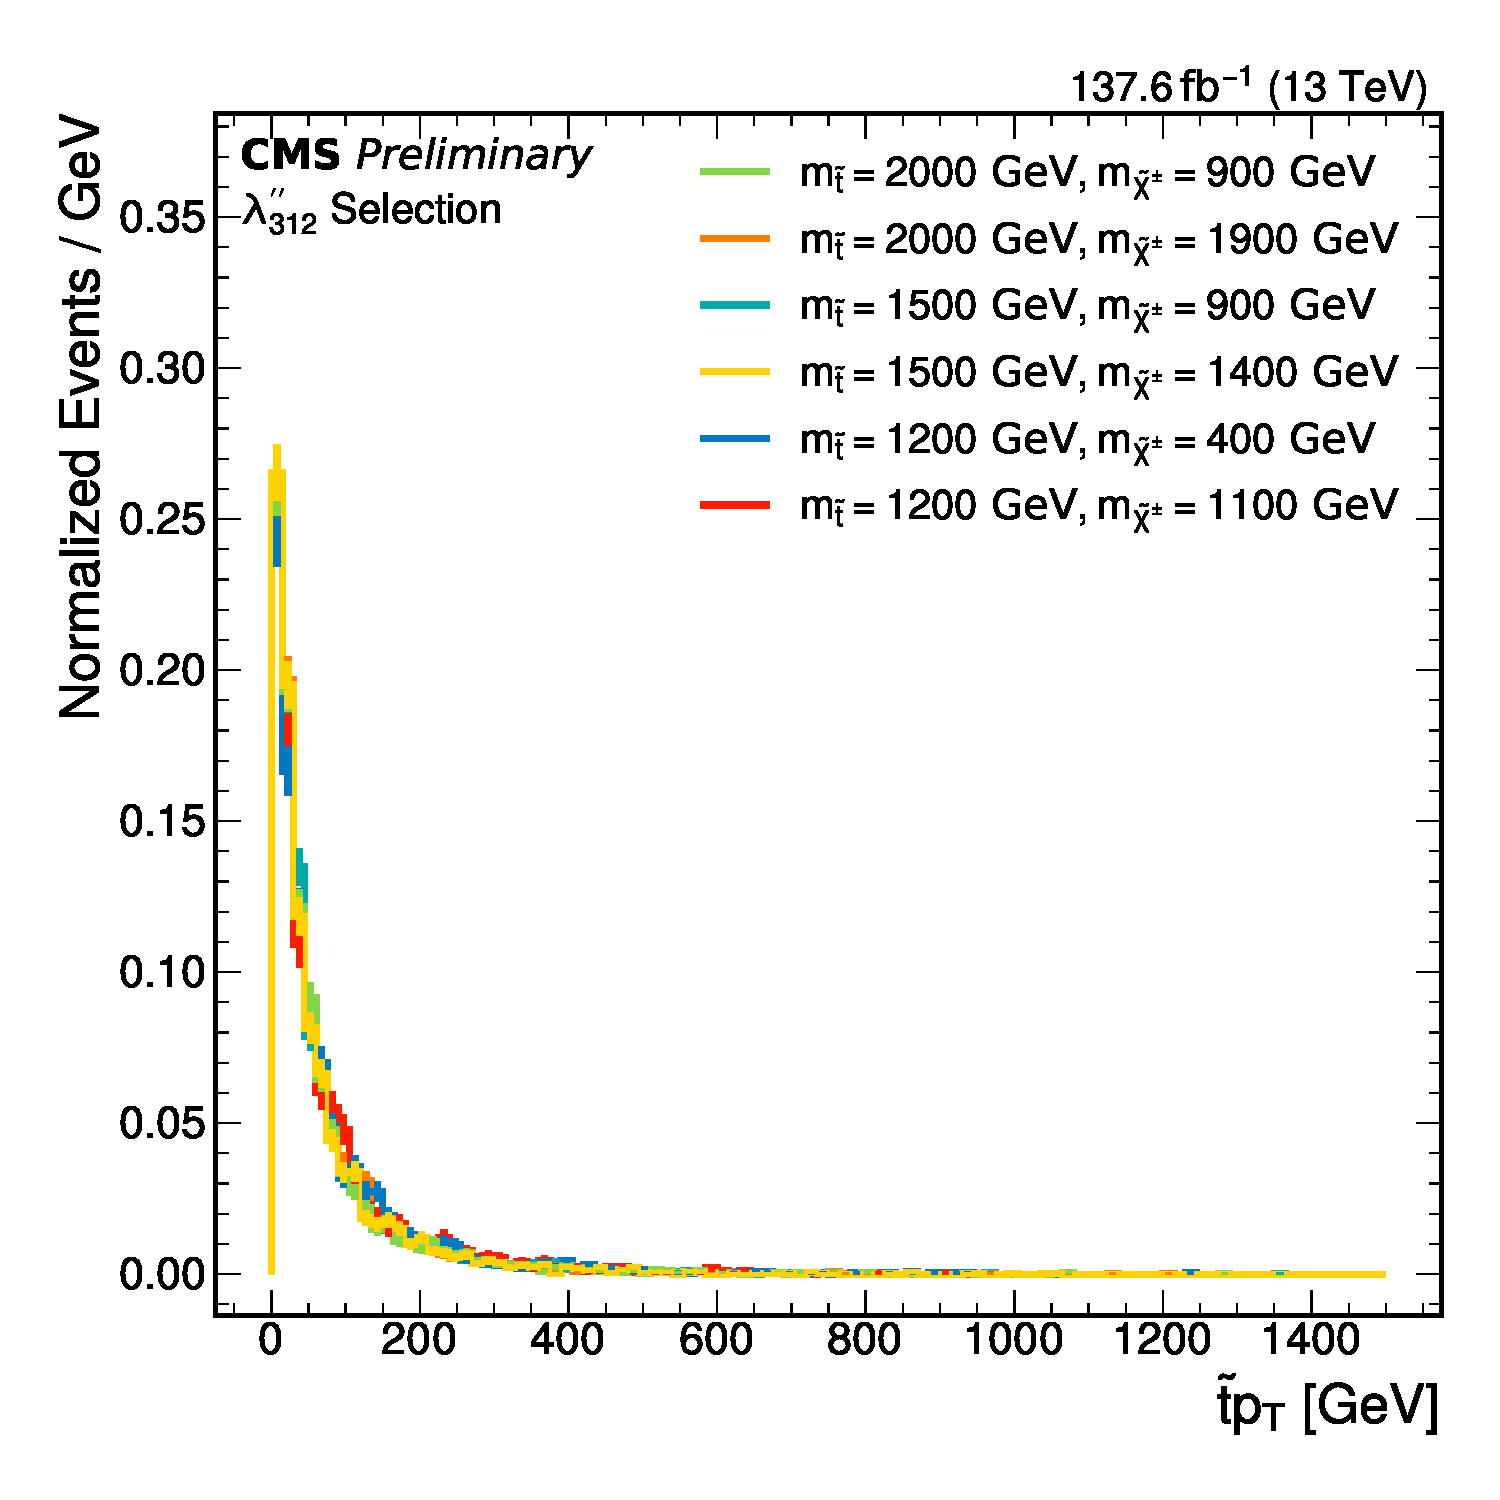
\includegraphics[width=0.08\textwidth]{figures/stop_pt.pdf}}}
      %\hlbox<3>{red}{\hyperlink{galleryslide<3>}{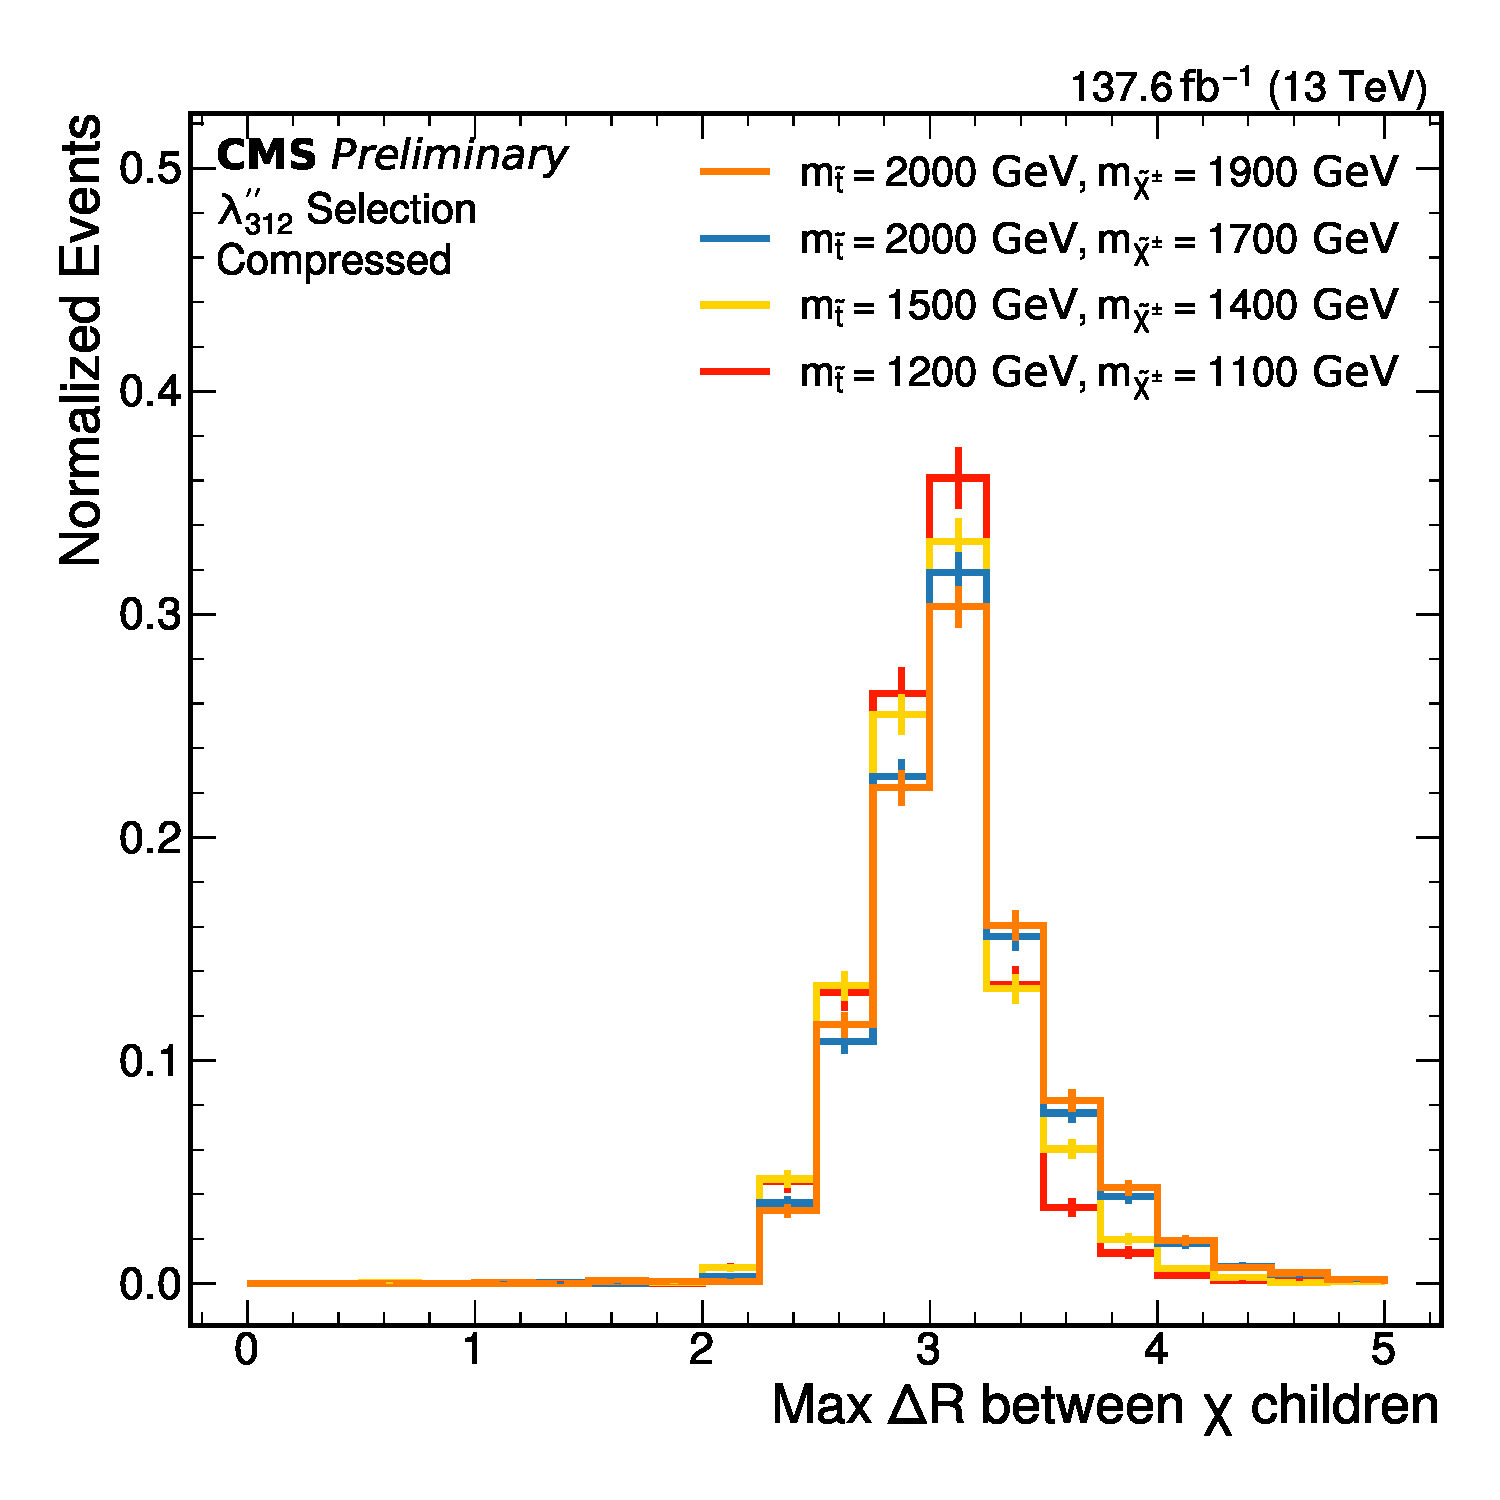
\includegraphics[width=0.08\textwidth]{figures/compressed_max_chi_child_dr.pdf} }}
      %\hlbox<3>{red}{\hyperlink{galleryslide<3>}{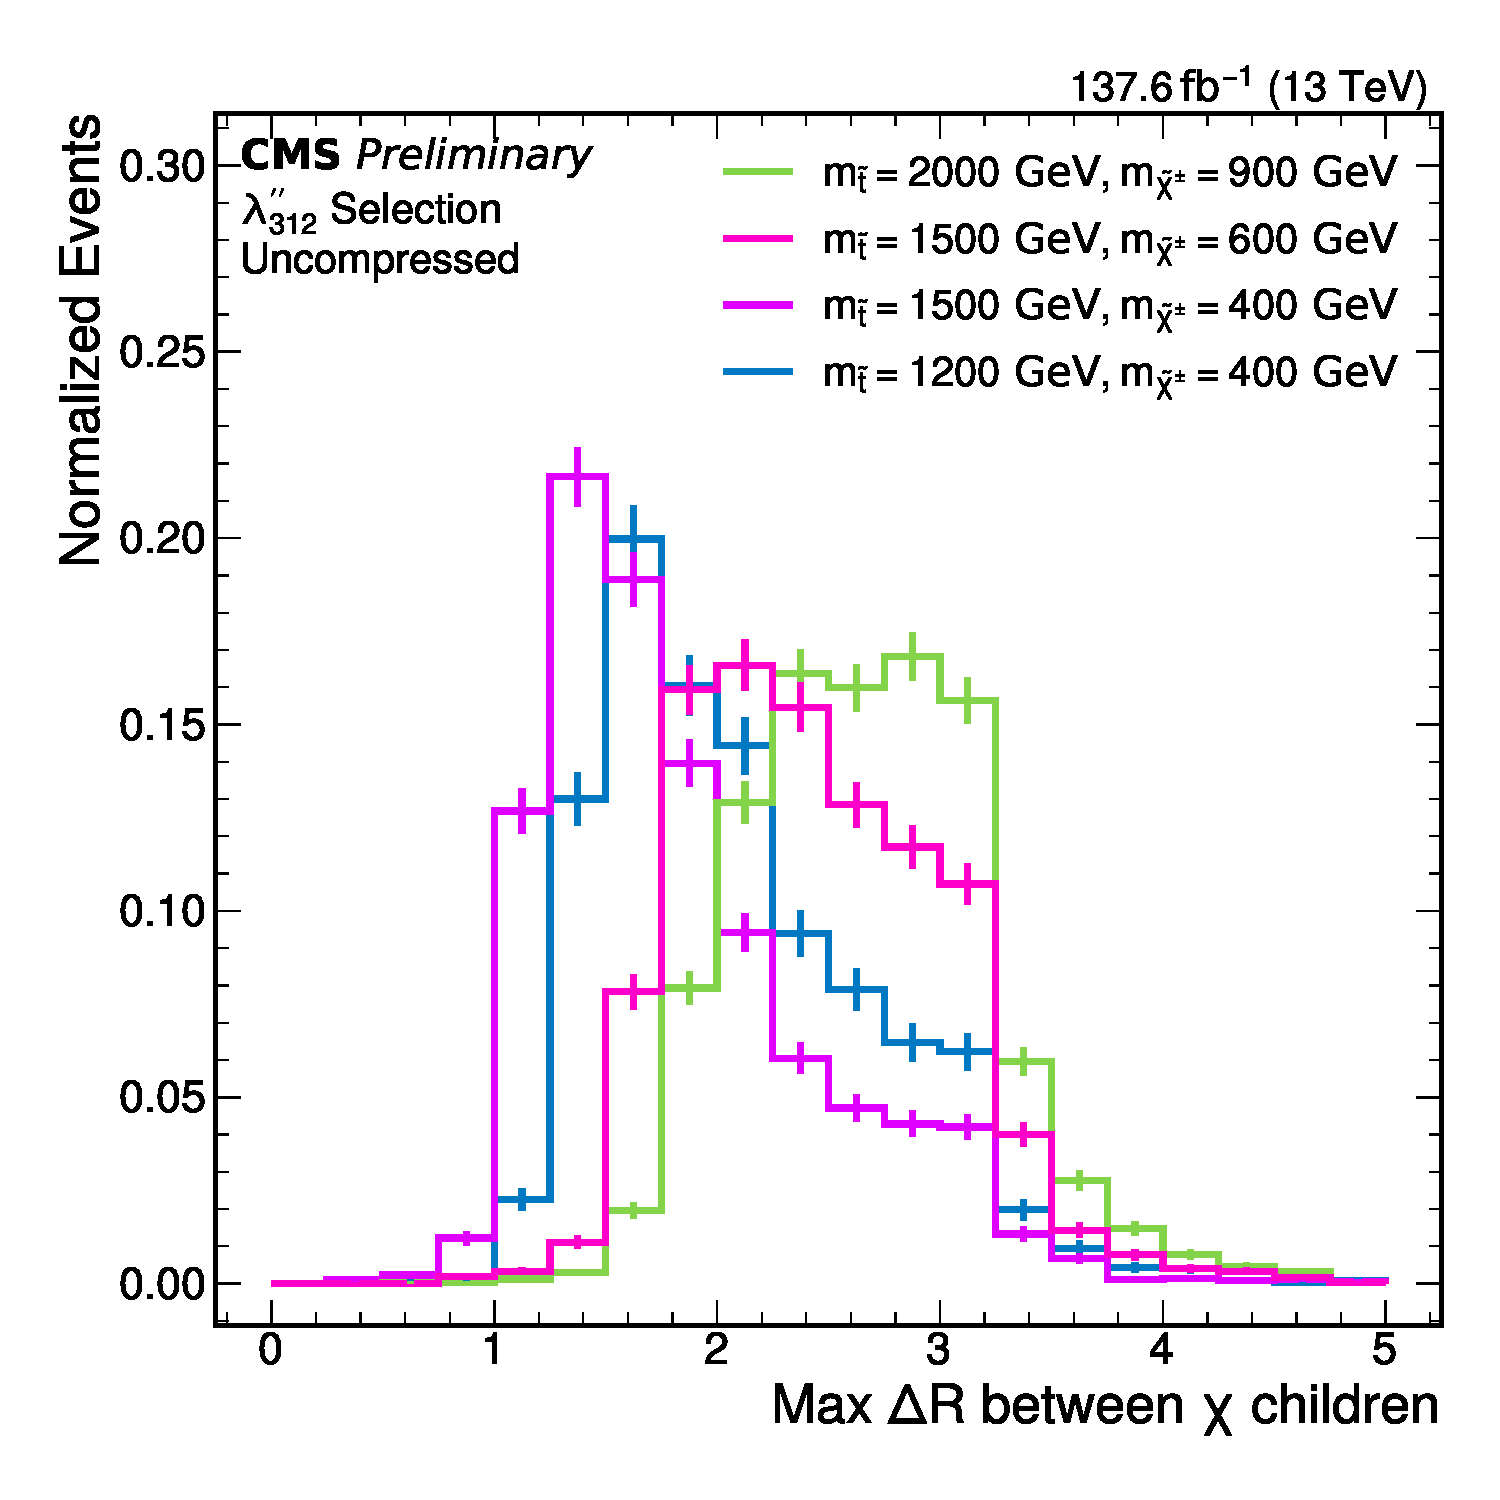
\includegraphics[width=0.08\textwidth]{figures/uncompressed_max_chi_child_dr.pdf} }}
      %\hlbox<4>{red}{\hyperlink{galleryslide<4>}{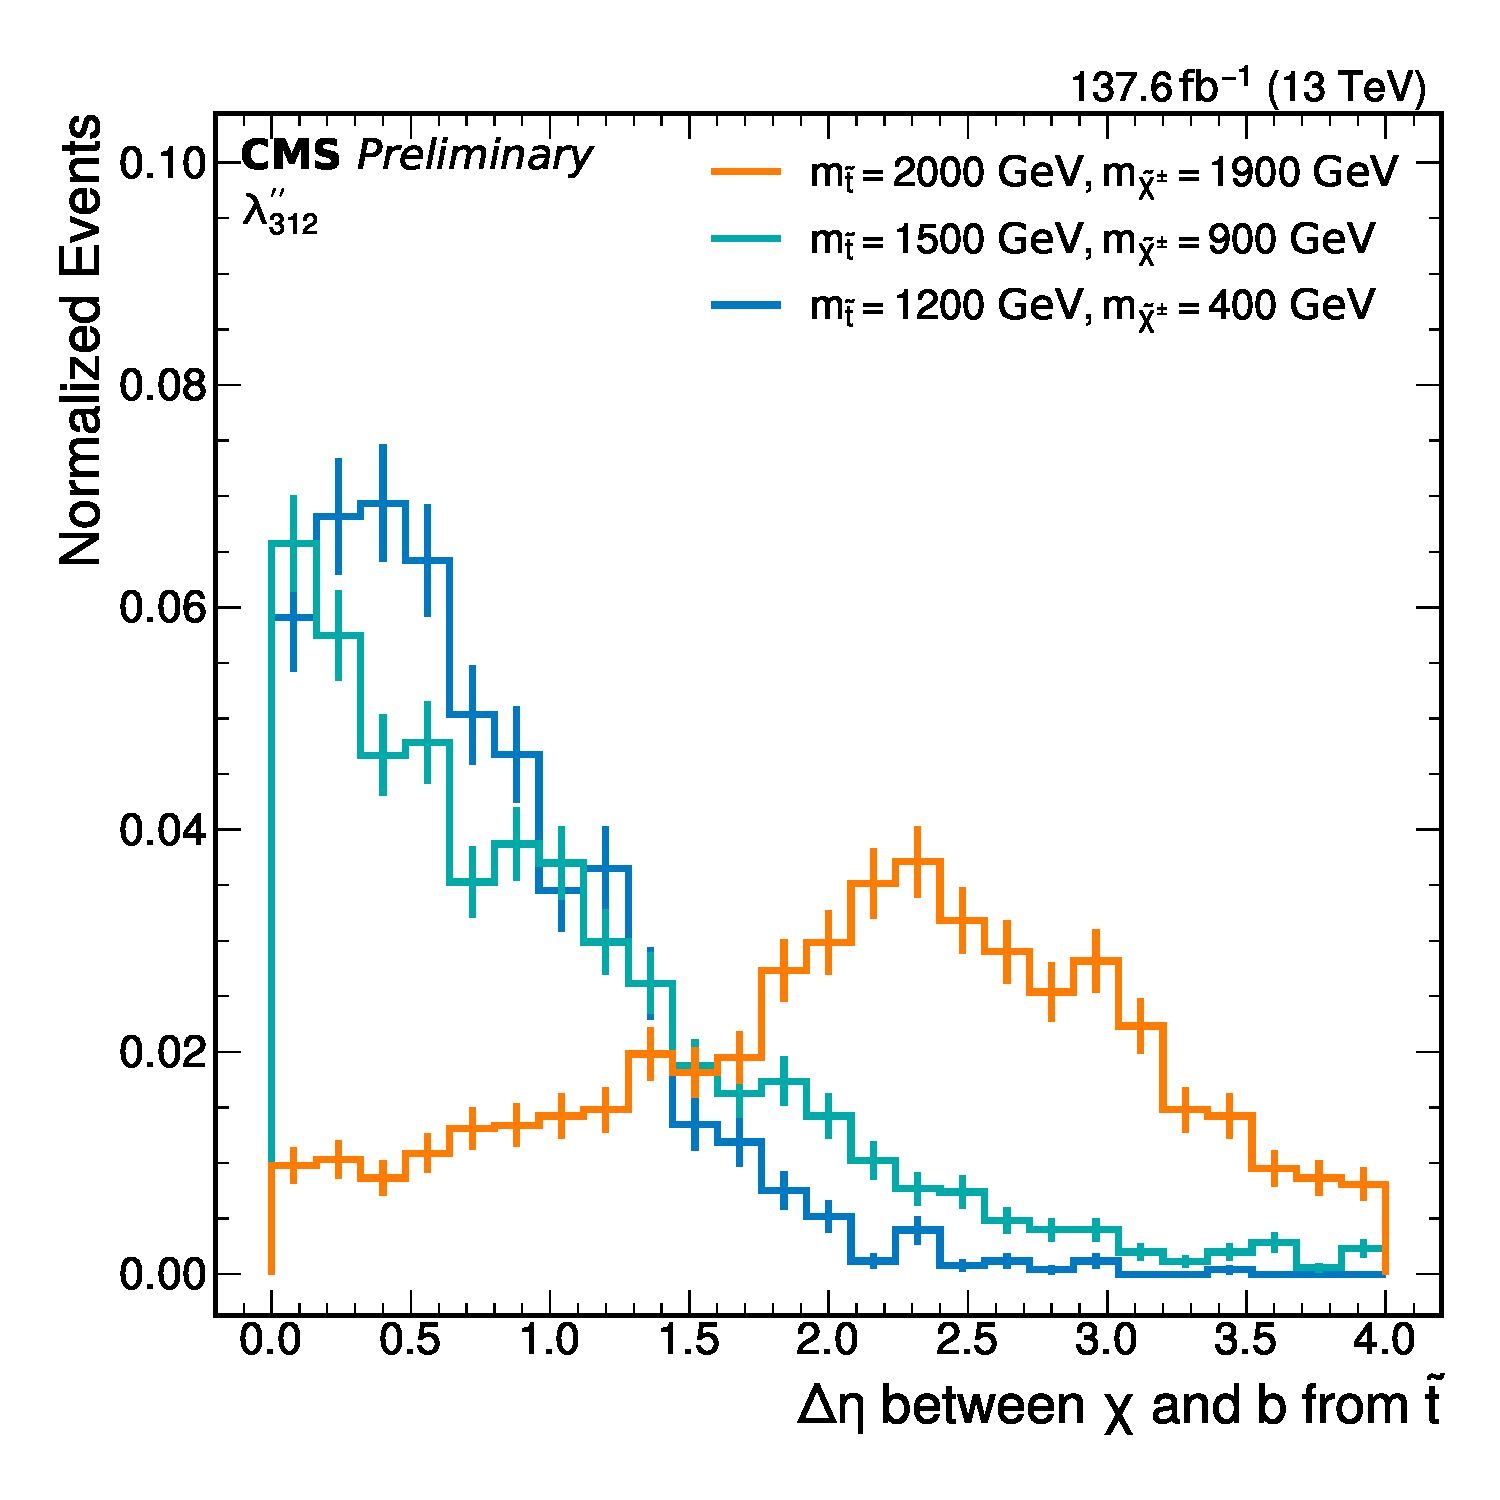
\includegraphics[width=0.08\textwidth]{figures/chi_b_eta.pdf} }}
      %\hlbox<4>{red}{\hyperlink{galleryslide<4>}{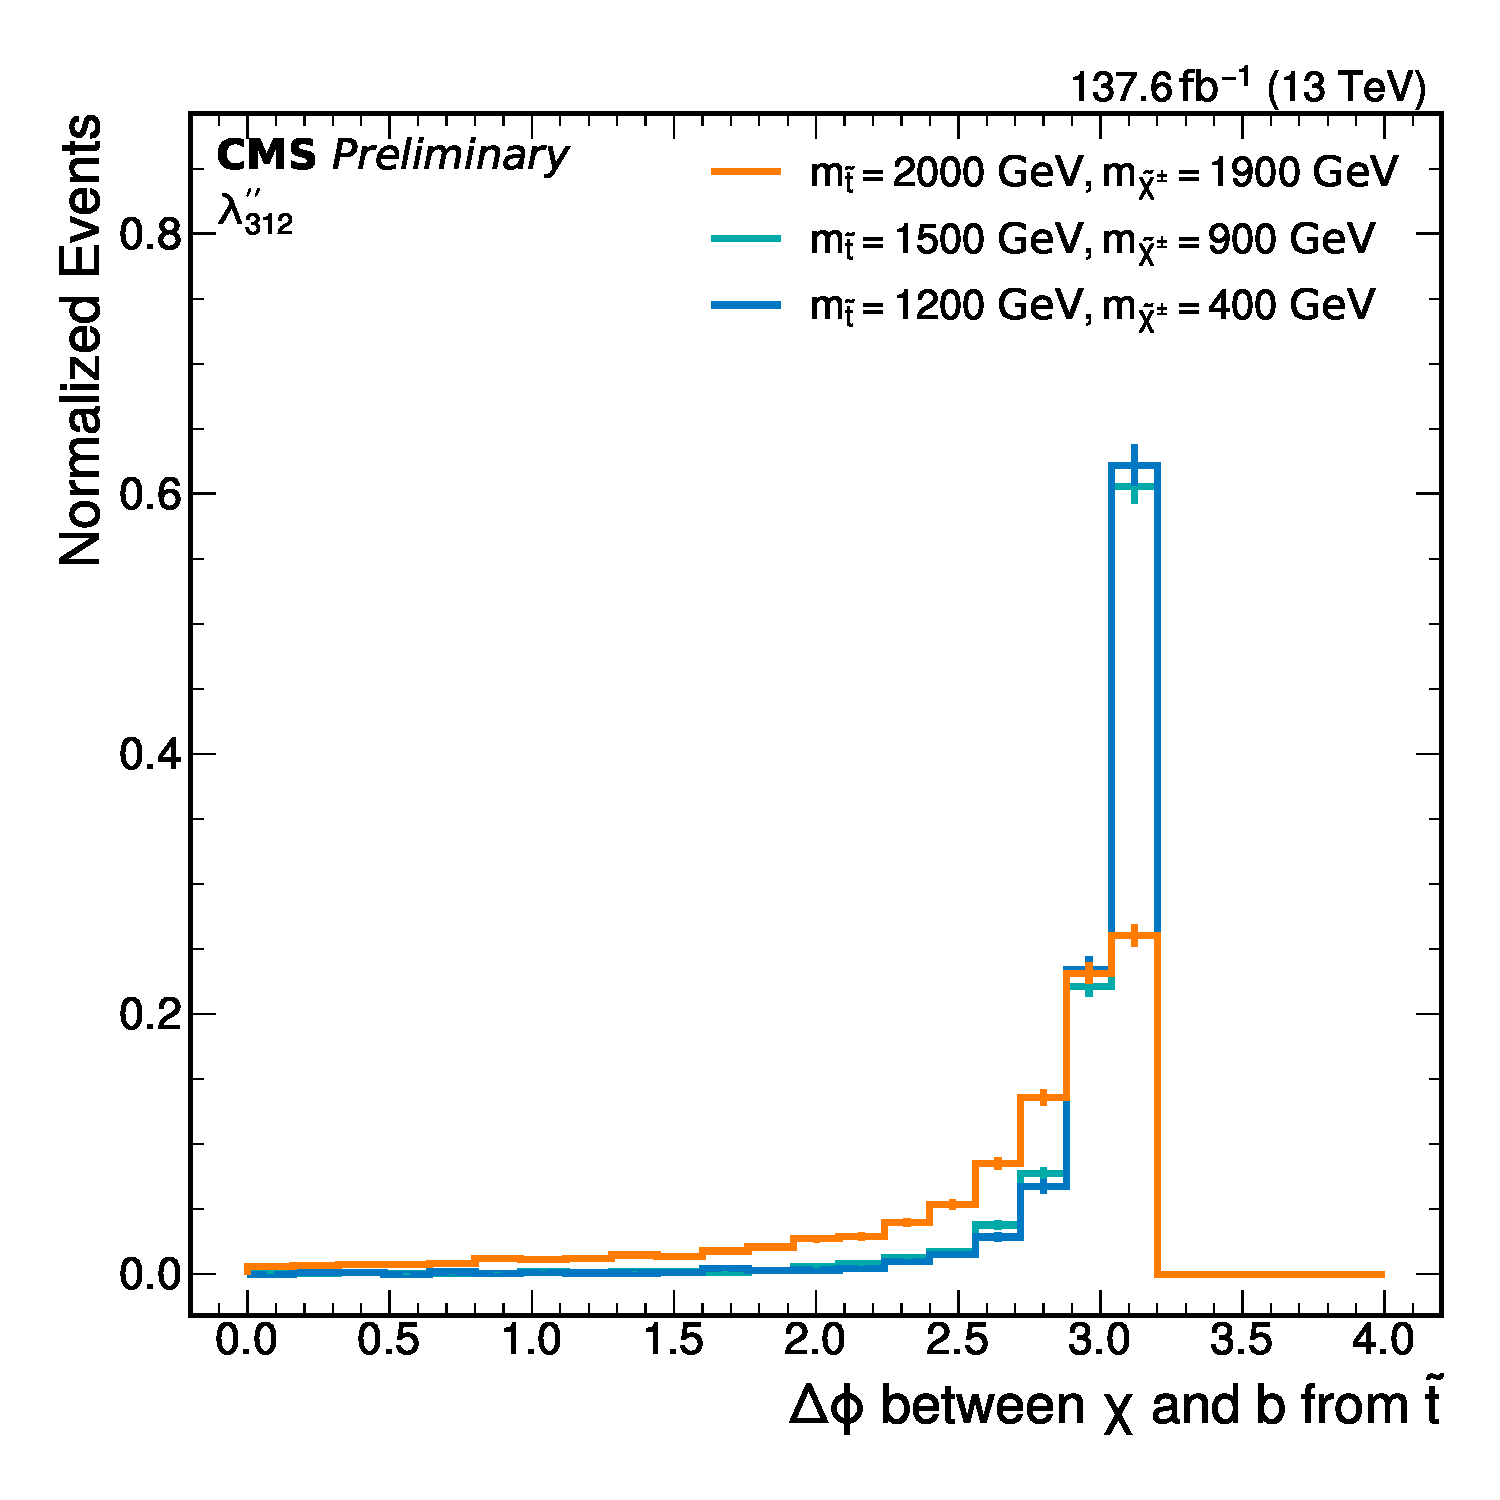
\includegraphics[width=0.08\textwidth]{figures/chi_b_phi.pdf} }}
      %\hlbox<4>{red}{\hyperlink{galleryslide<4>}{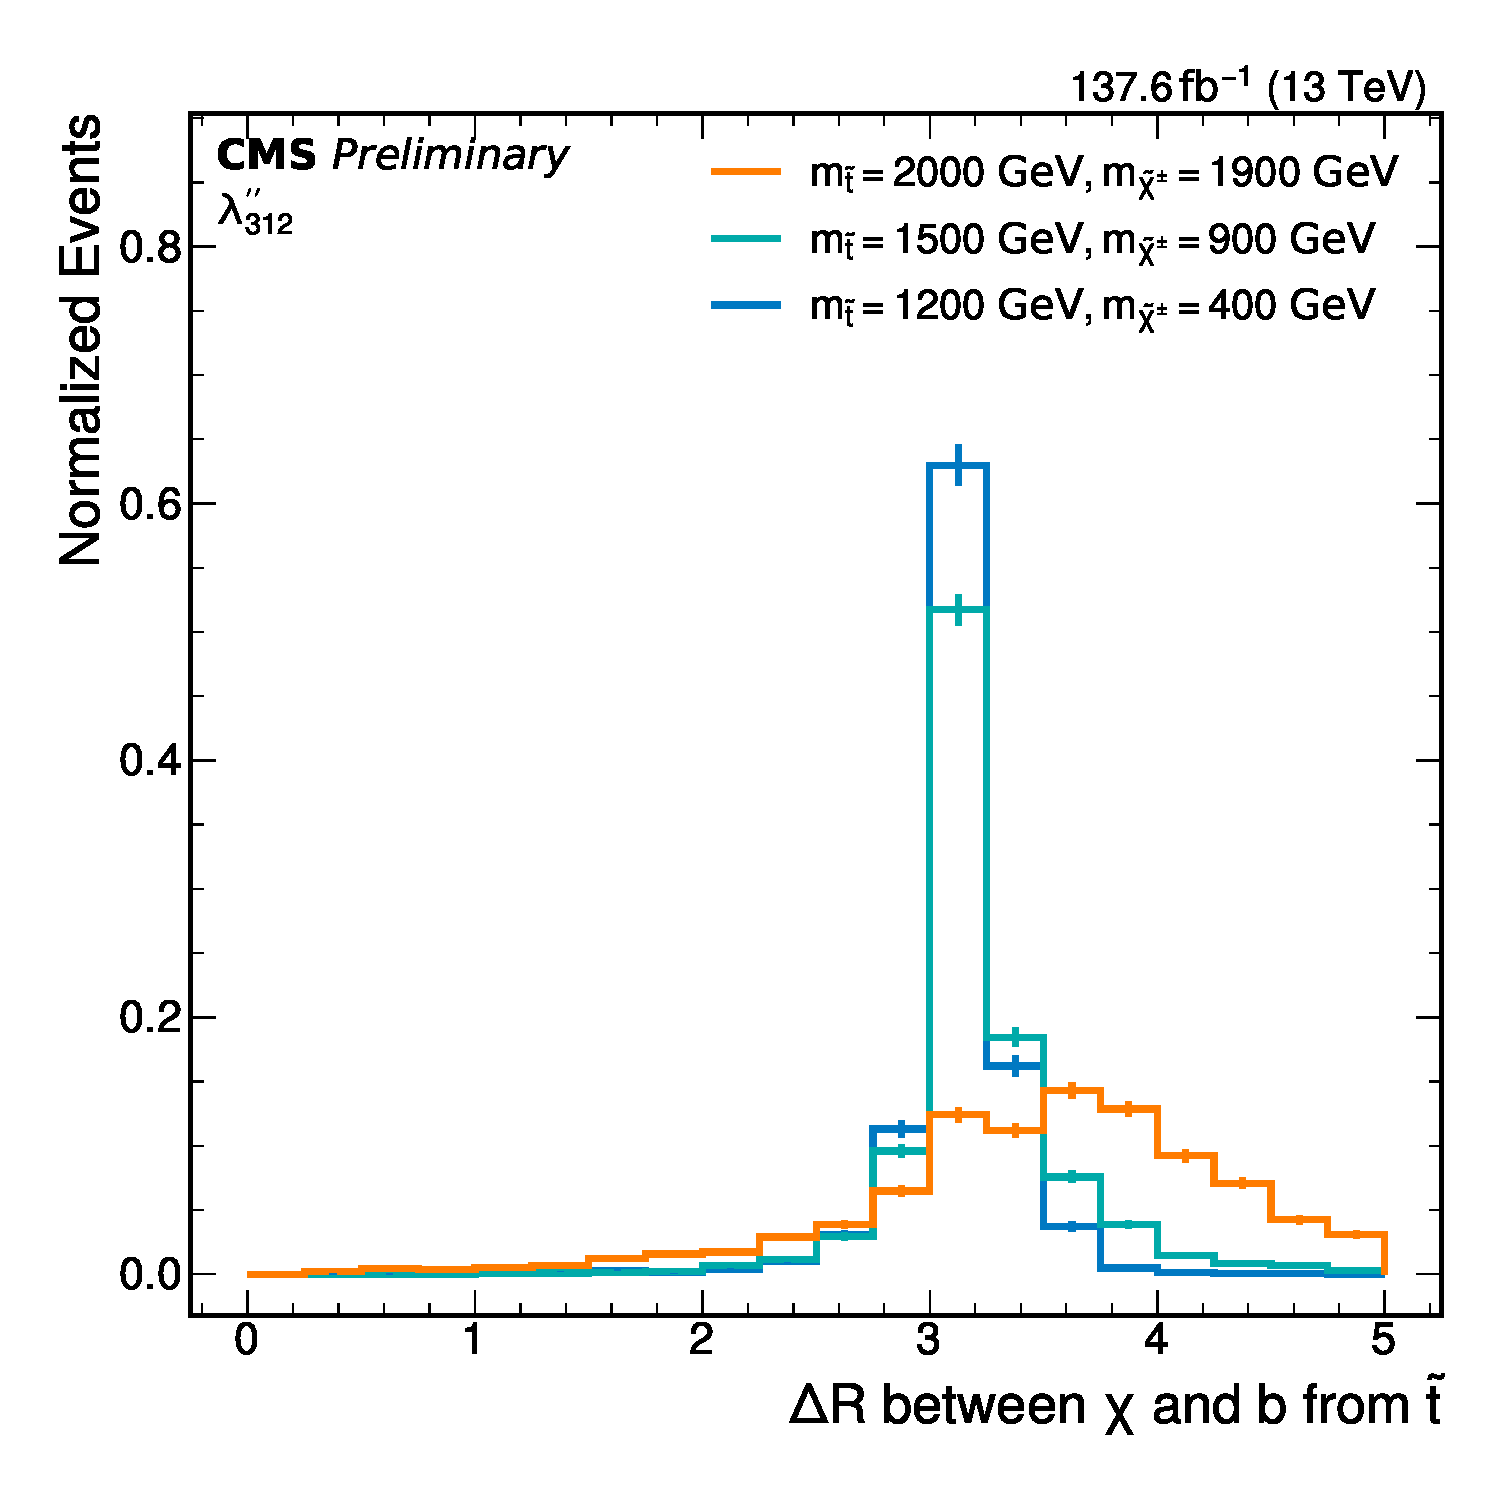
\includegraphics[width=0.08\textwidth]{figures/chi_b_dr.pdf} }}
      %\hlbox<5>{red}{\hyperlink{galleryslide<5>}{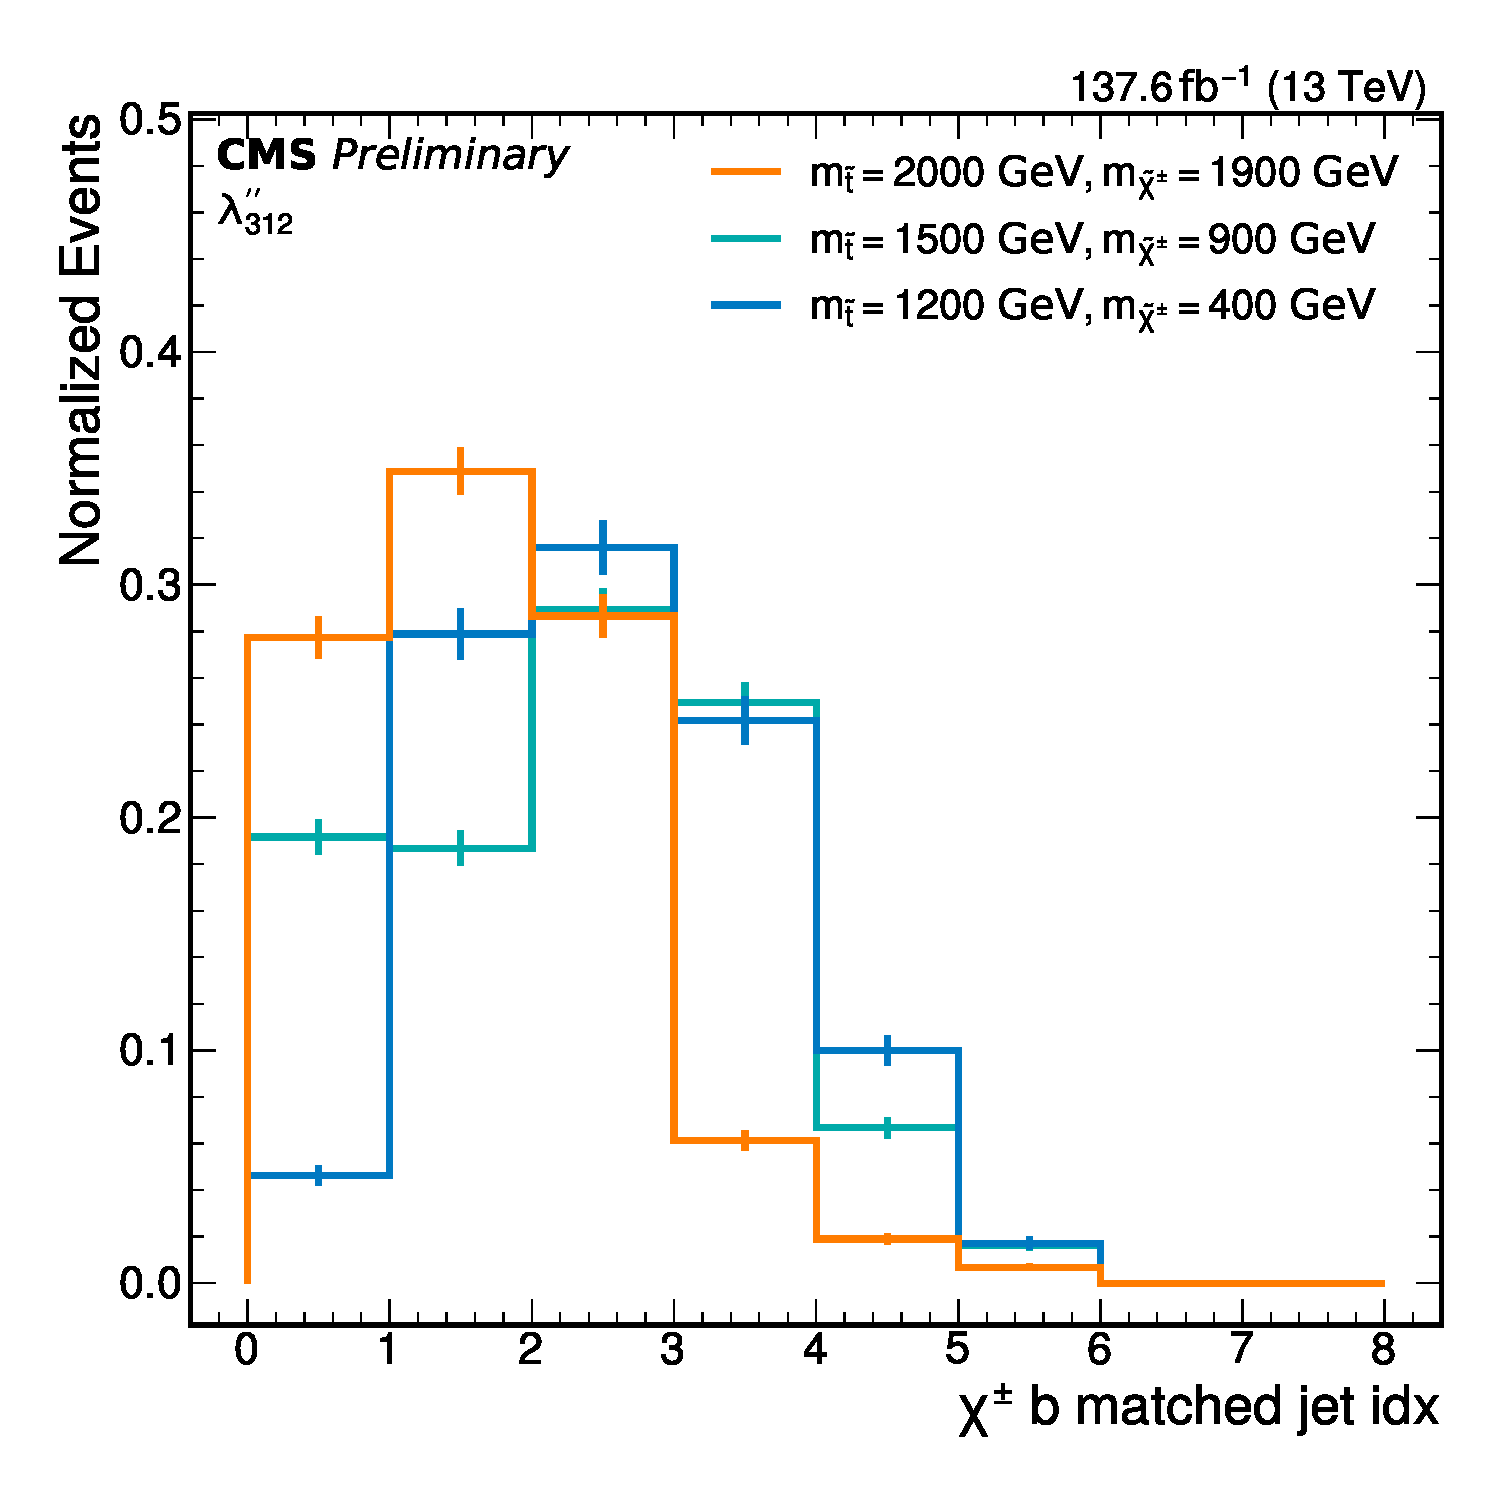
\includegraphics[width=0.08\textwidth]{figures/chi_b_jet_idx.pdf} }}
      %\hlbox<5>{red}{\hyperlink{galleryslide<5>}{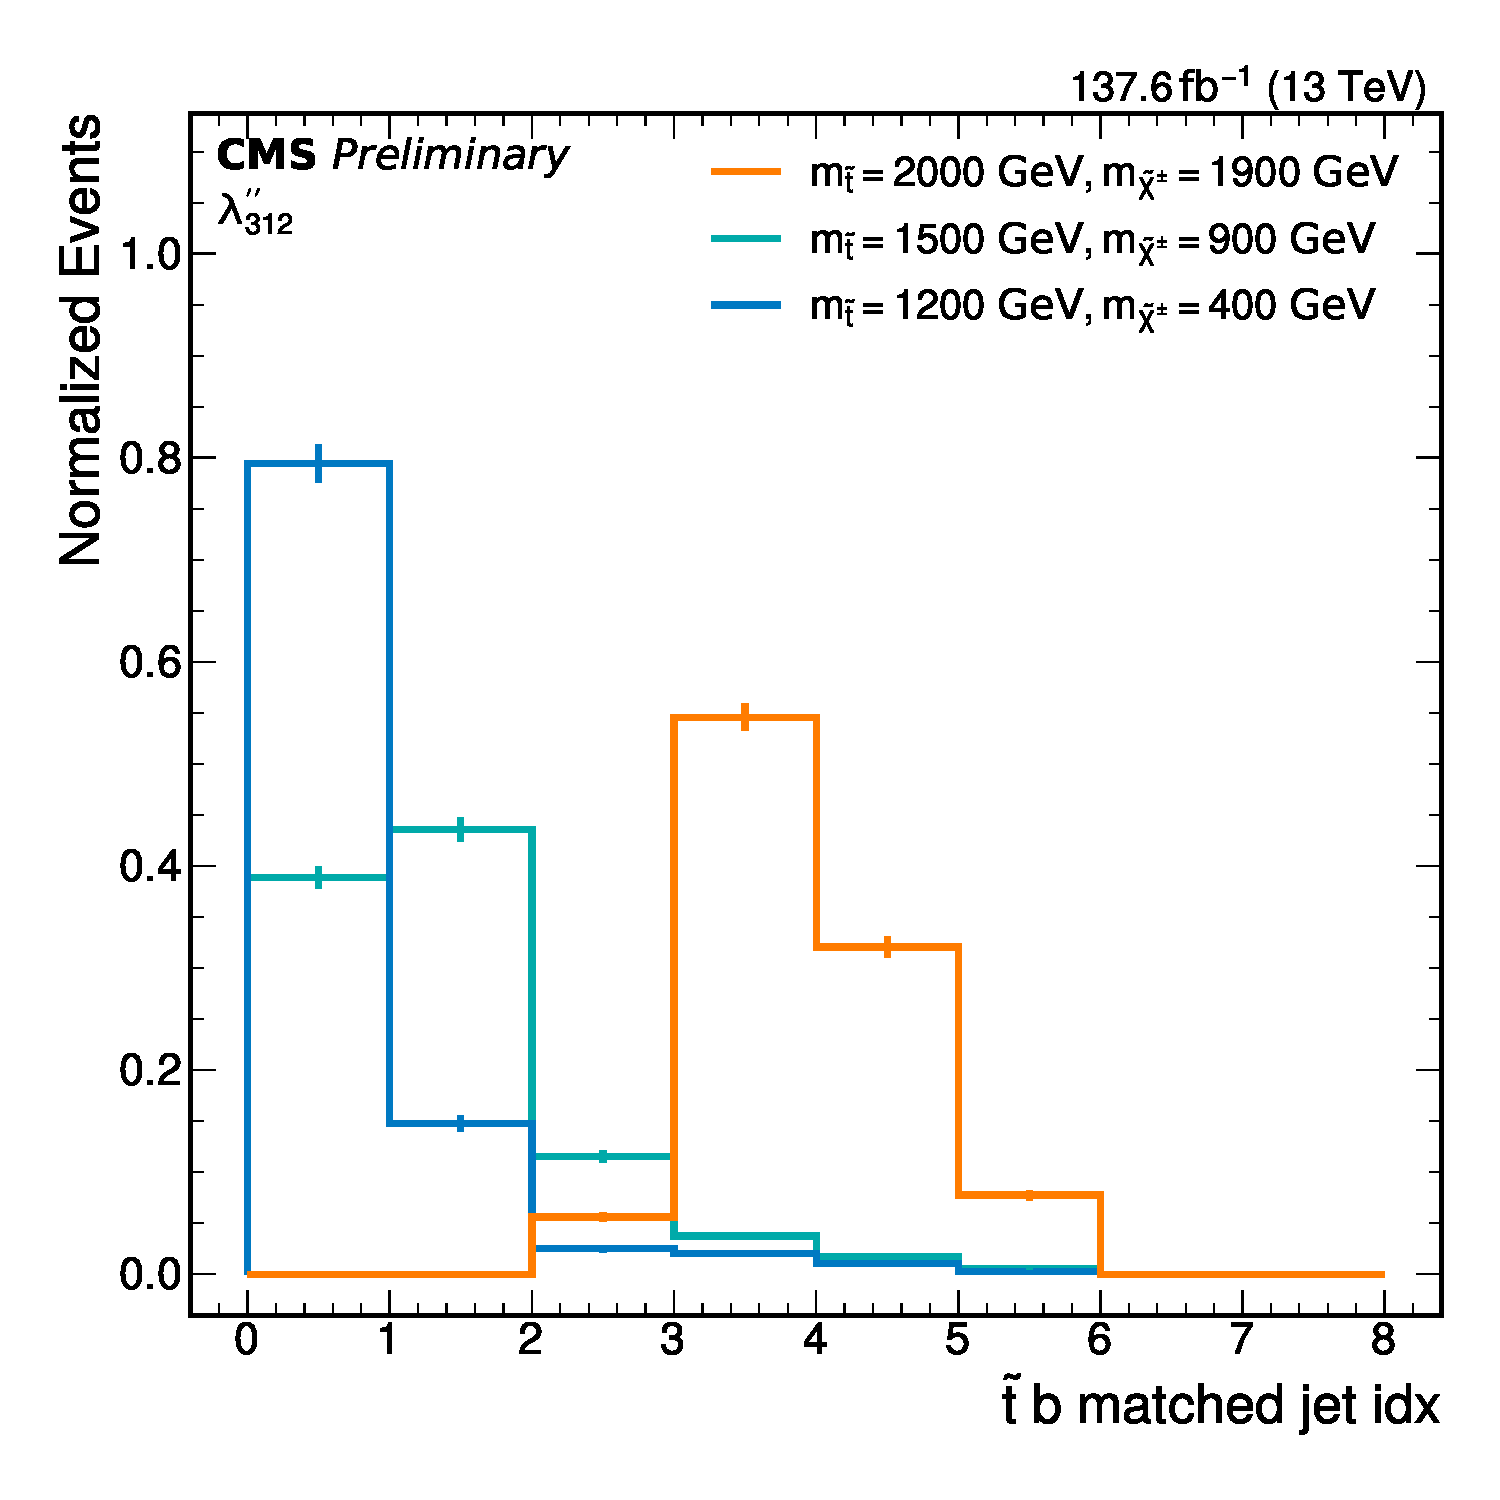
\includegraphics[width=0.08\textwidth]{figures/stop_b_jet_idx.pdf} }}
      % \end{onlyenv}
      % \end{center}
    \begin{overlayarea}{\textwidth}{2.5cm}
      \begin{columns}
        \begin{column}{0.3\textwidth}
          \scalebox{0.45}{
            \begin{tikzpicture} 
              \drawdiagram{$d_{i}$}{$d_{j}$}
            \end{tikzpicture}}
        \end{column}
        \begin{column}{0.7\textwidth}
          \begin{onlyenv}<2> The \stopq{} is produced nearly at rest in the transverse plane. \end{onlyenv}
          \begin{onlyenv}<3> The maximum angular separation between any two of the \chargino{} children. The less compressed a mass point, the more collimated the children. \end{onlyenv}
          \begin{onlyenv}<4> The two \stopq{} children have large angular separation, consistent with single particle decay. \end{onlyenv}
          \begin{onlyenv}<5> In the compressed category, the \chargino{} \quarkb{} is often one of the leading (highest $p_{T}$) three jets. In the uncompressed category, the \stopq{} \quarkb{} is often the leading jet. \end{onlyenv}
        \end{column}
      \end{columns}
    \end{overlayarea}
    % \begin{overlayarea}{\textwidth}{2cm}
    \begin{center}
      \begin{onlyenv}<2>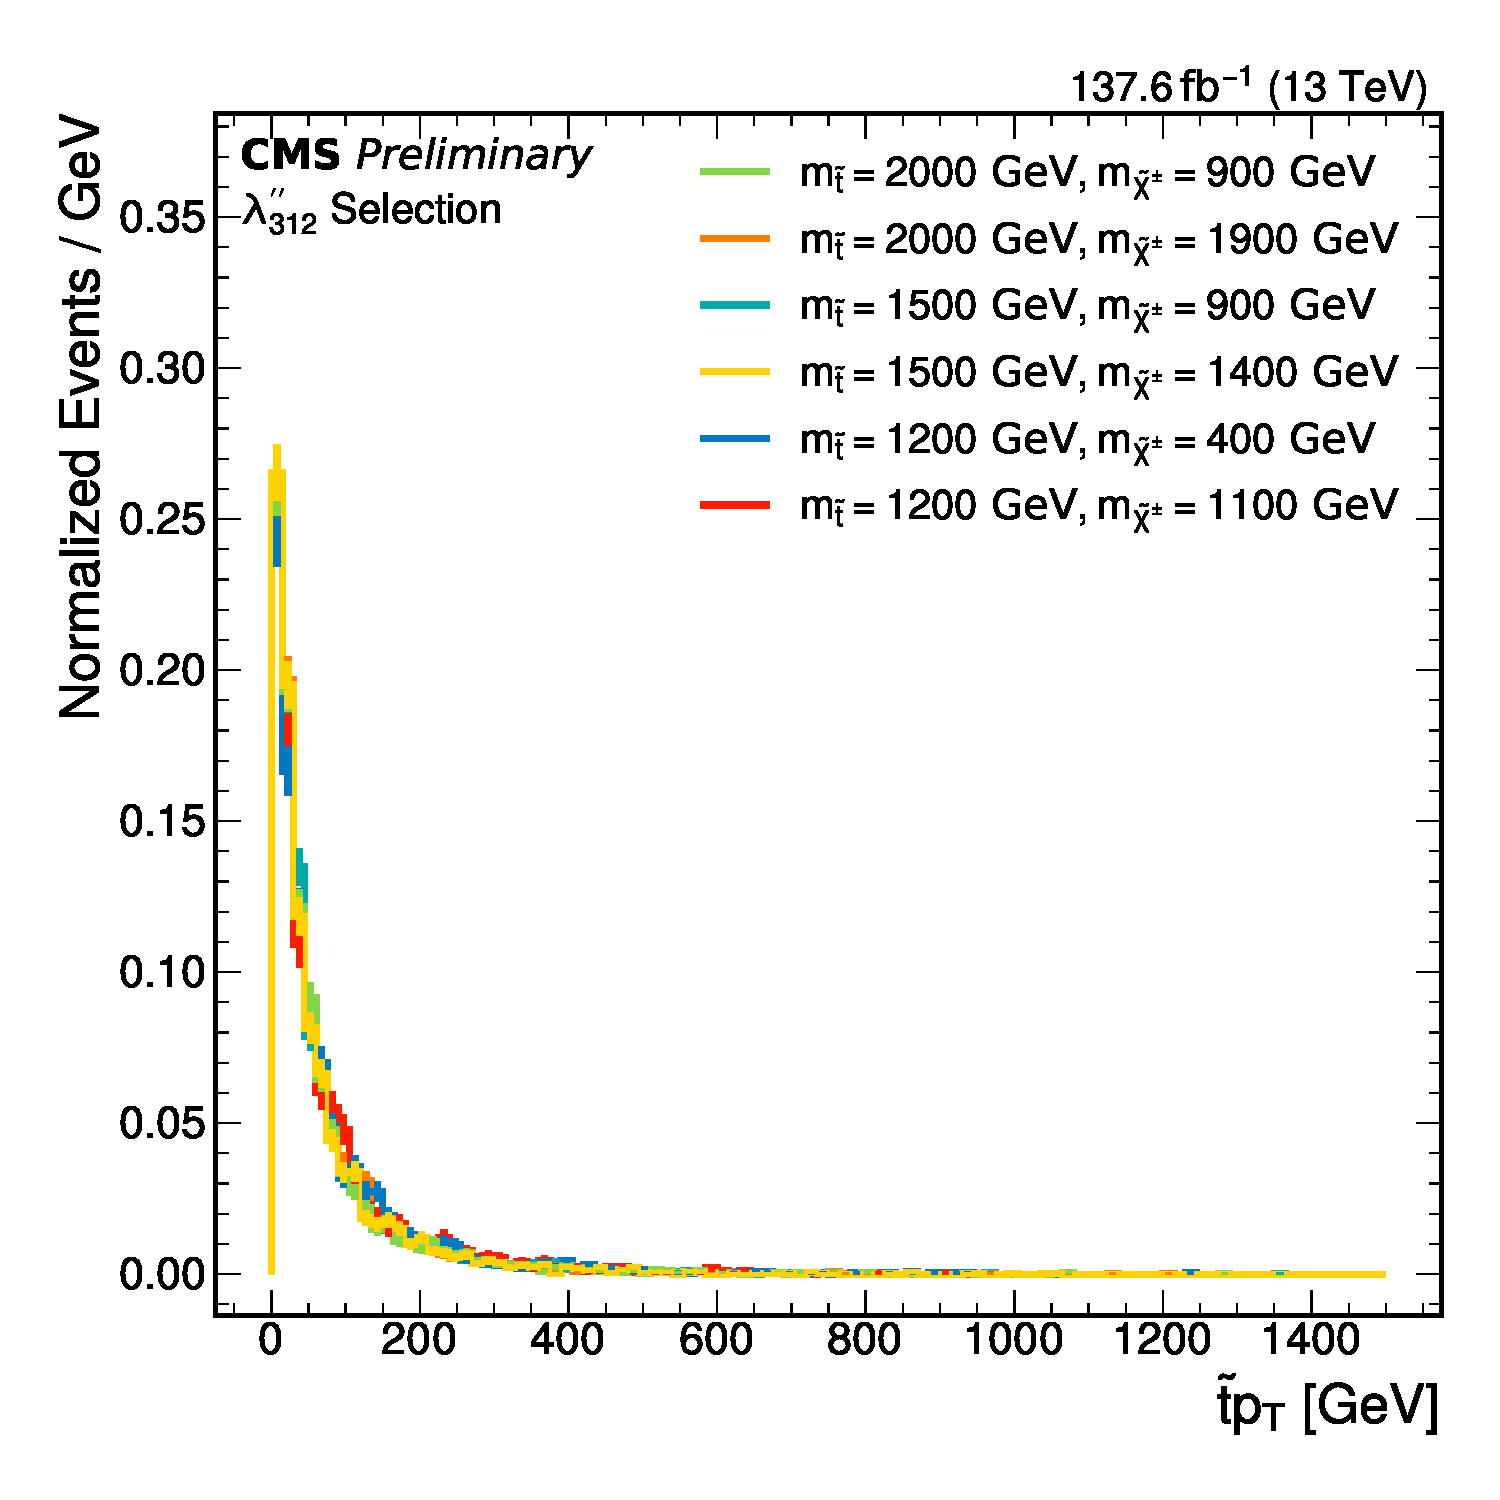
\includegraphics[width=0.4\textwidth]{figures/stop_pt.pdf}\end{onlyenv}
      \begin{onlyenv}<3>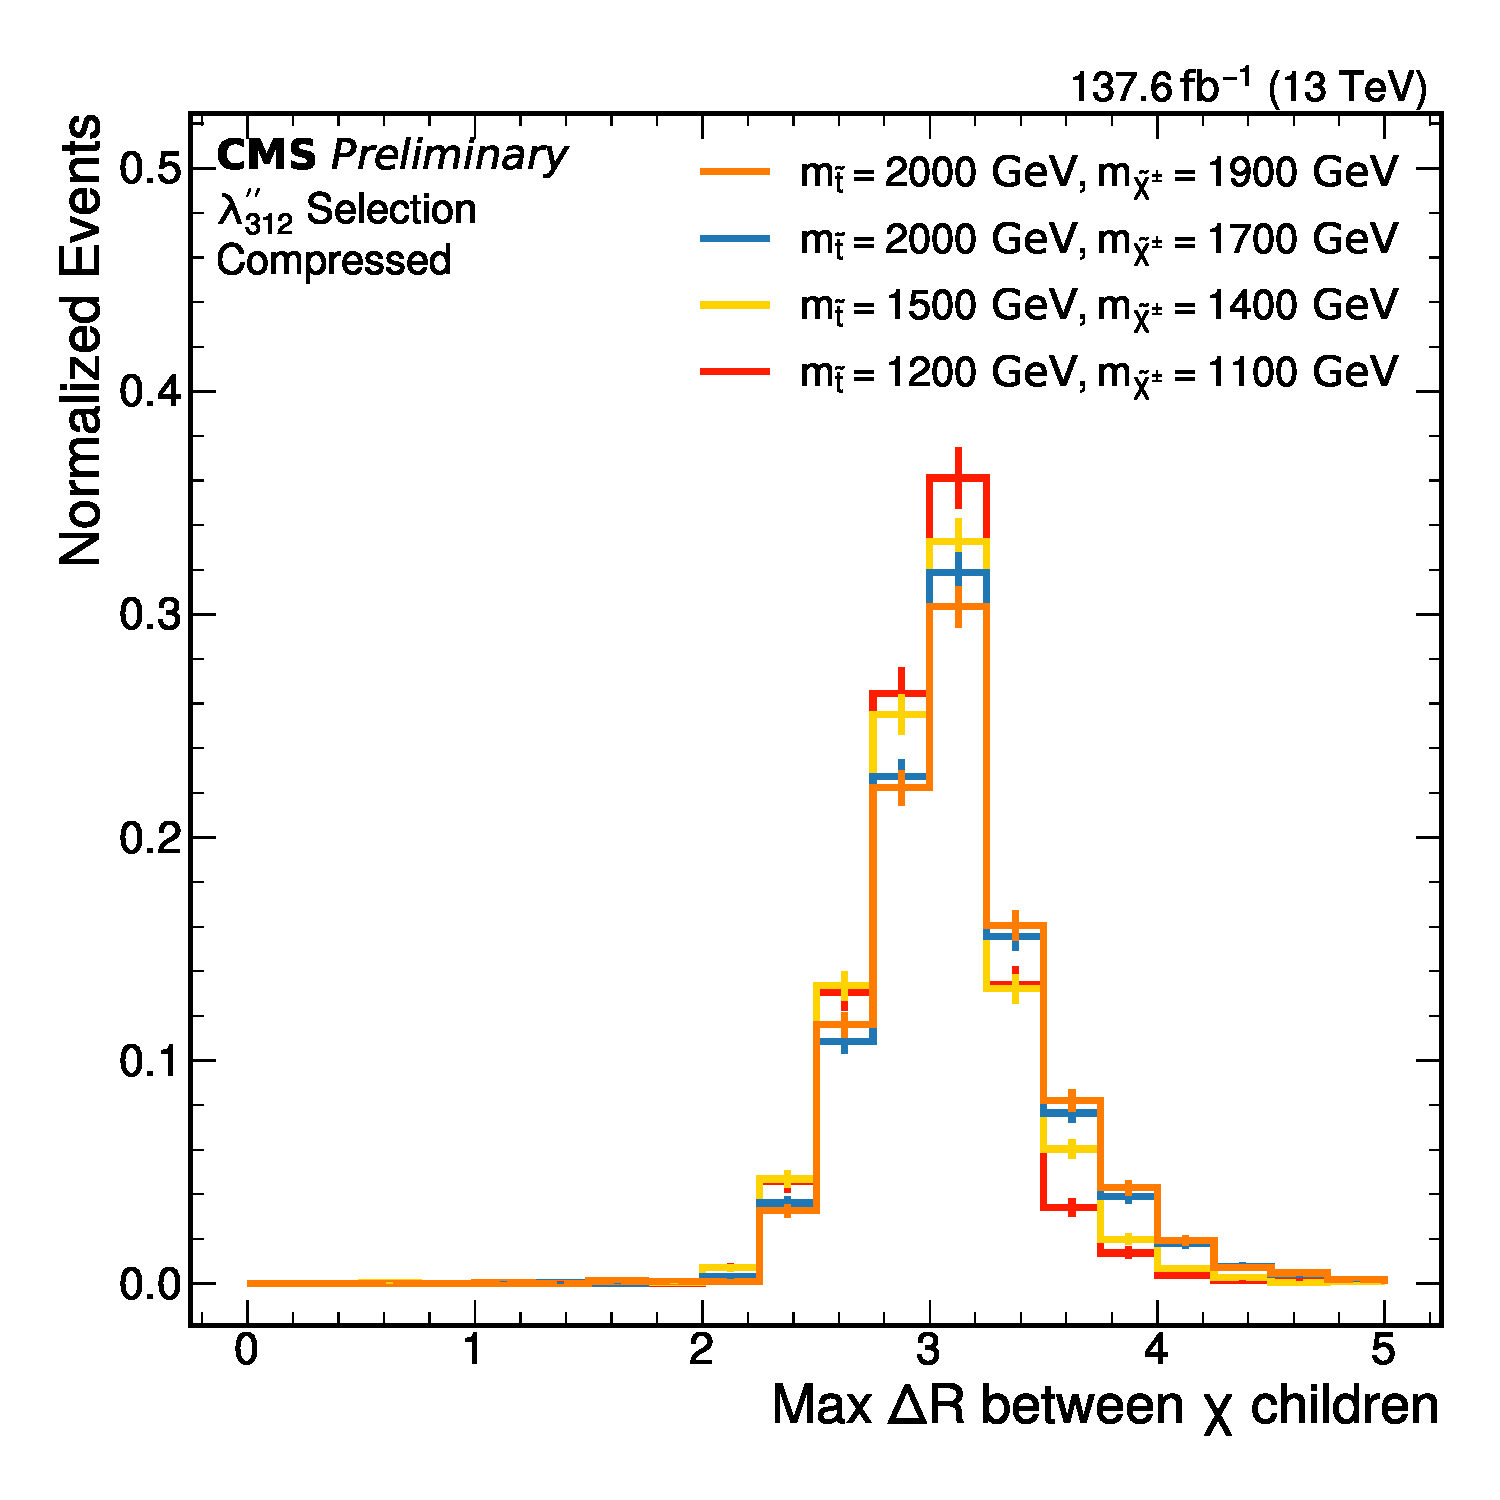
\includegraphics[width=0.4\textwidth]{figures/compressed_max_chi_child_dr.pdf} \end{onlyenv}
      \begin{onlyenv}<3>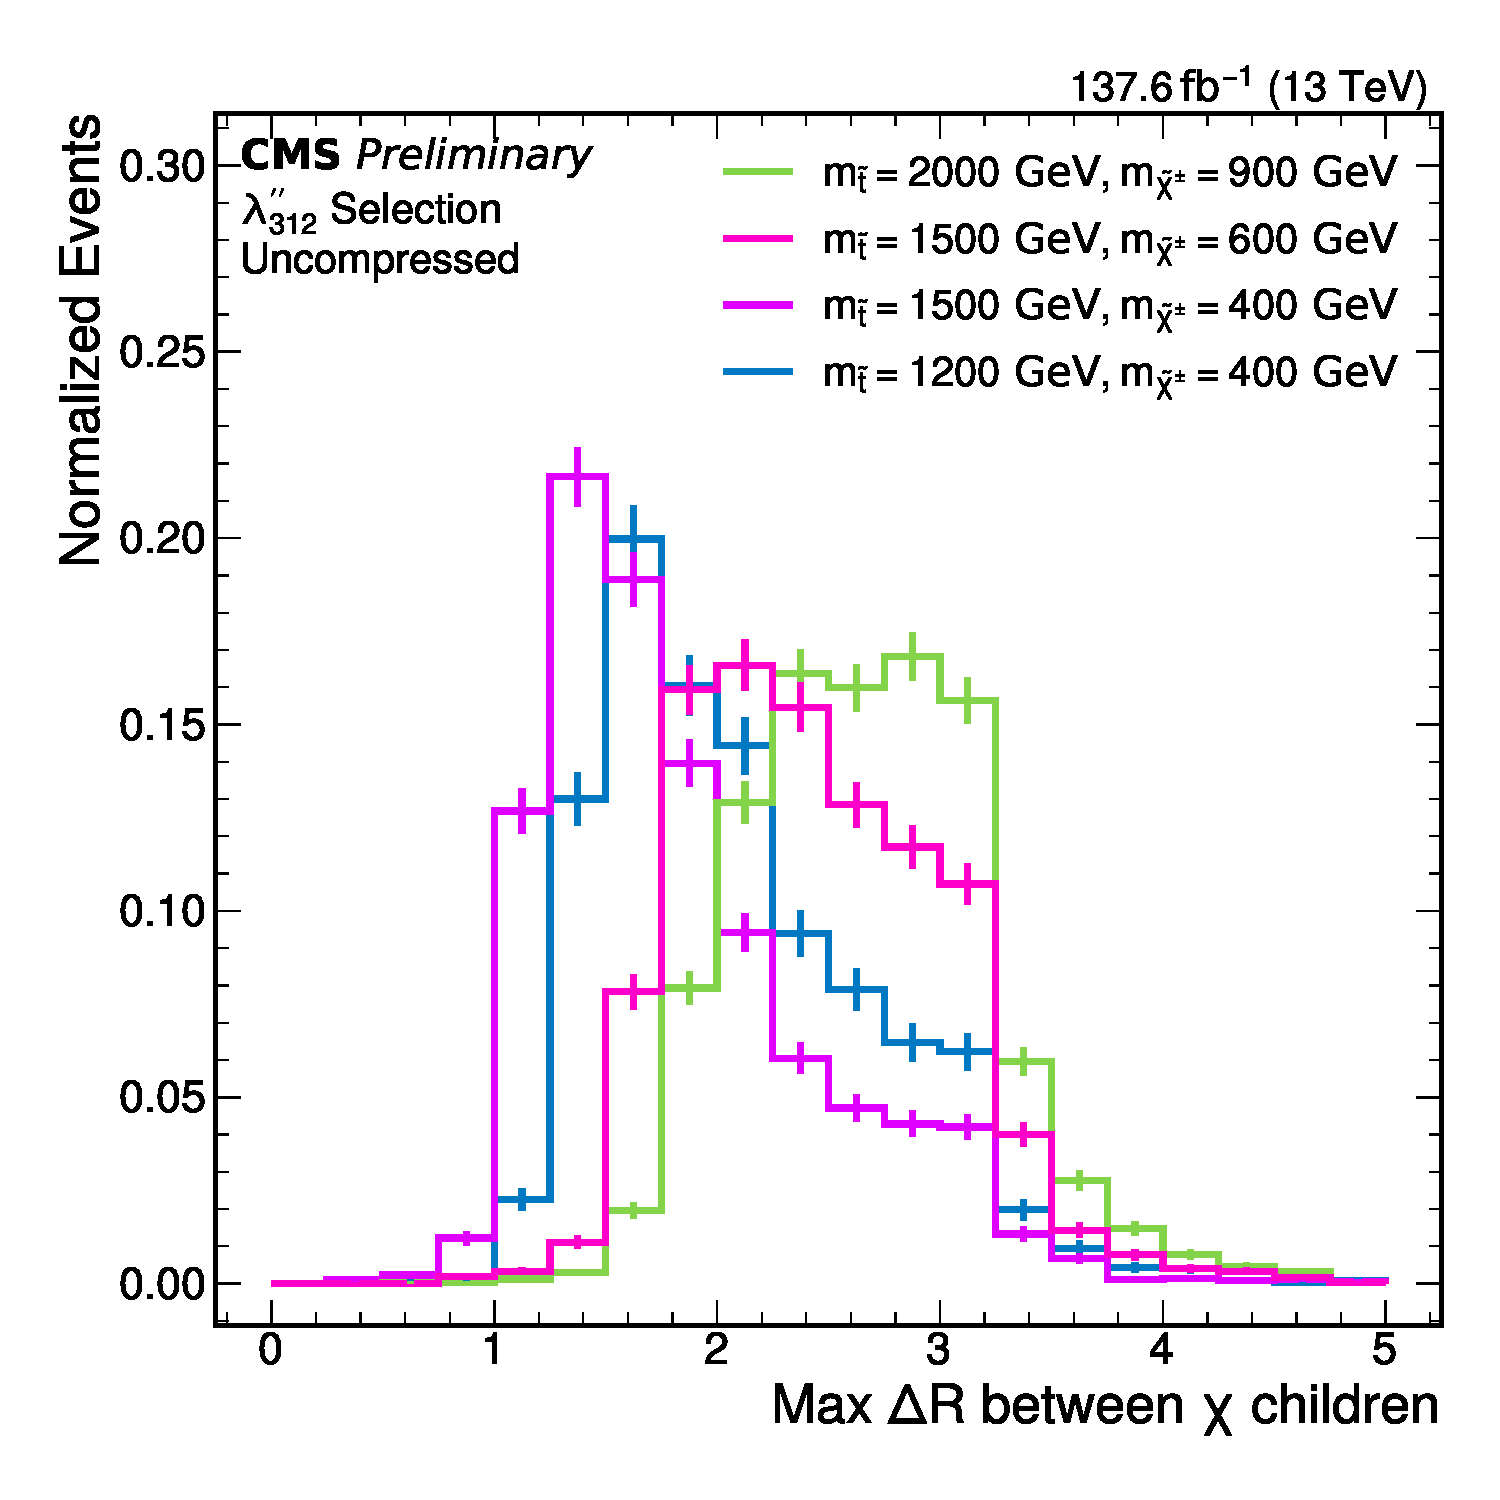
\includegraphics[width=0.4\textwidth]{figures/uncompressed_max_chi_child_dr.pdf} \end{onlyenv}
      \begin{onlyenv}<4>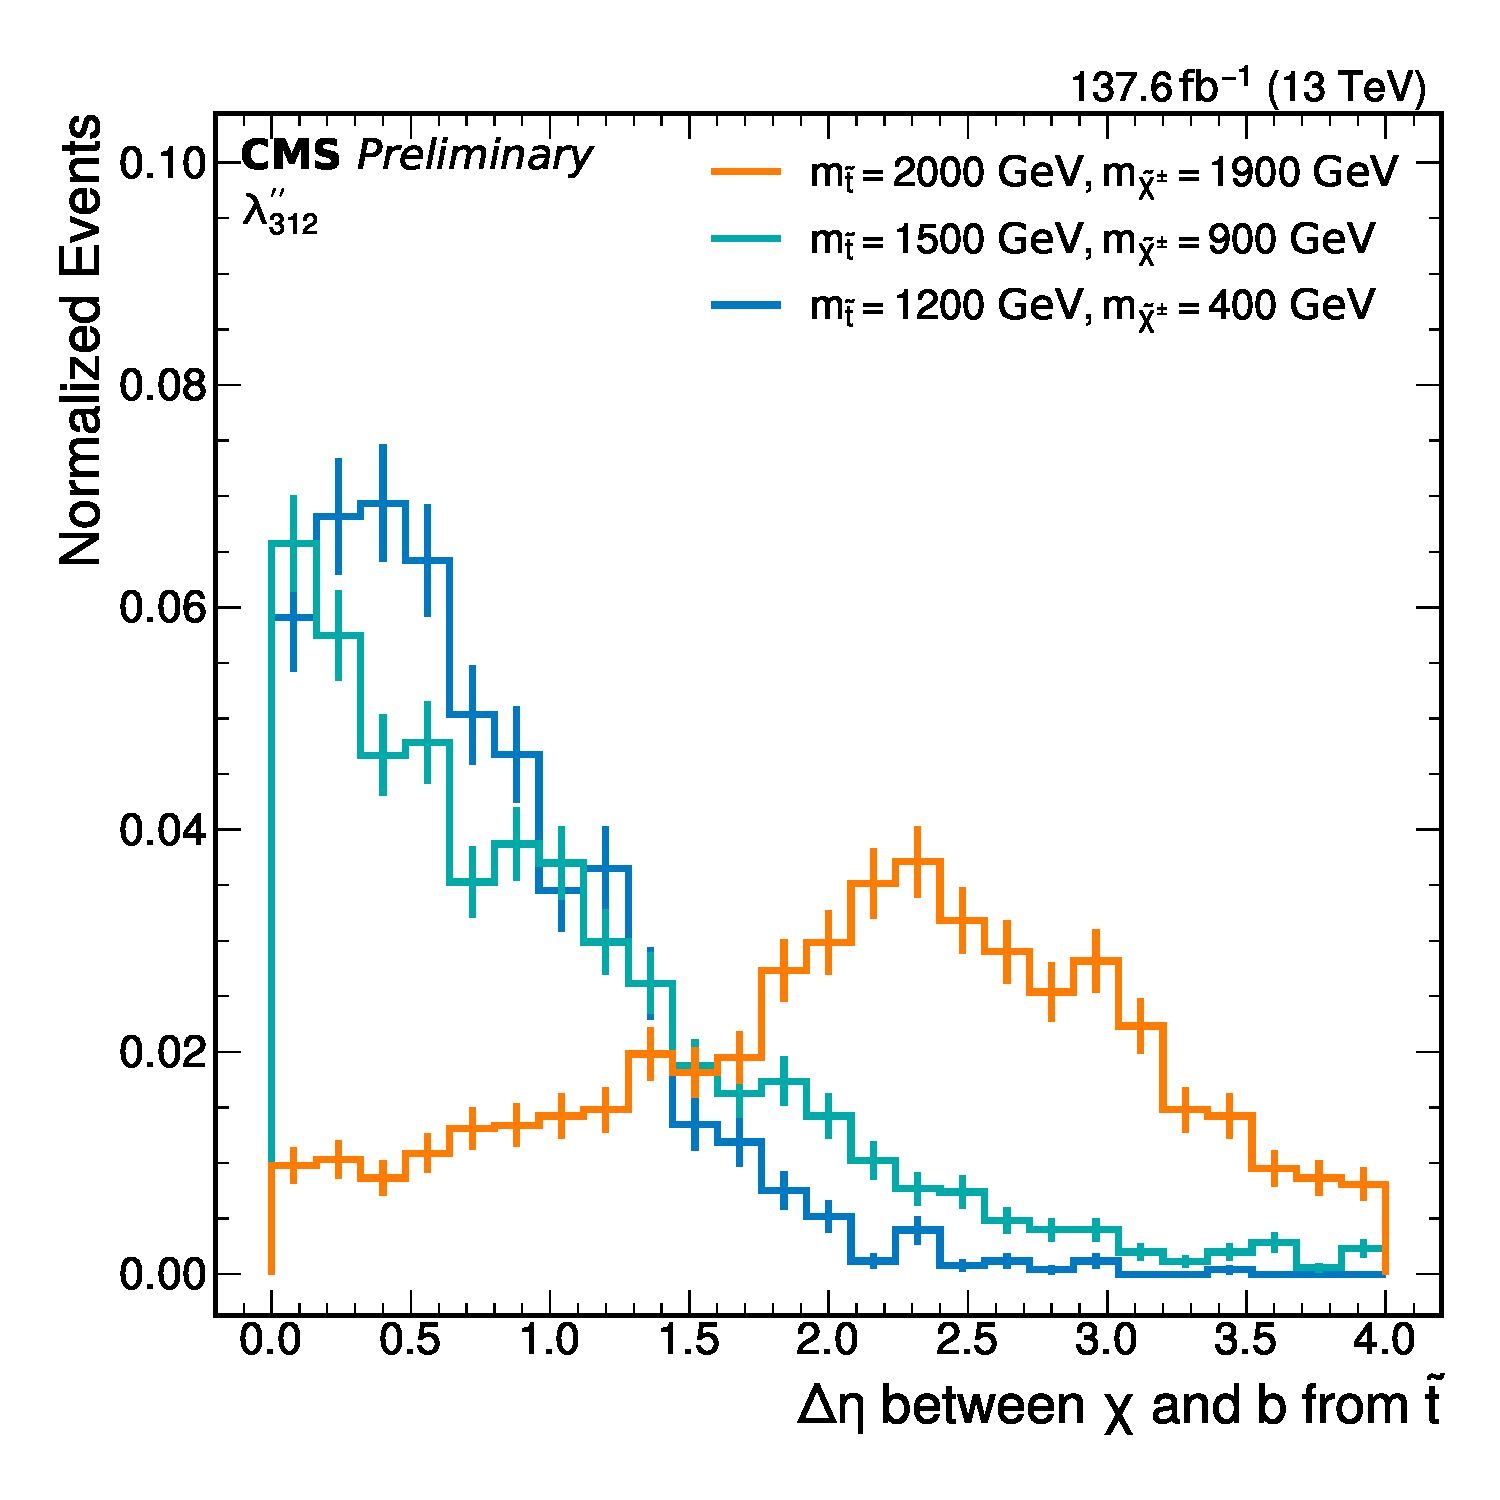
\includegraphics[width=0.3\textwidth]{figures/chi_b_eta.pdf} \end{onlyenv}
      \begin{onlyenv}<4>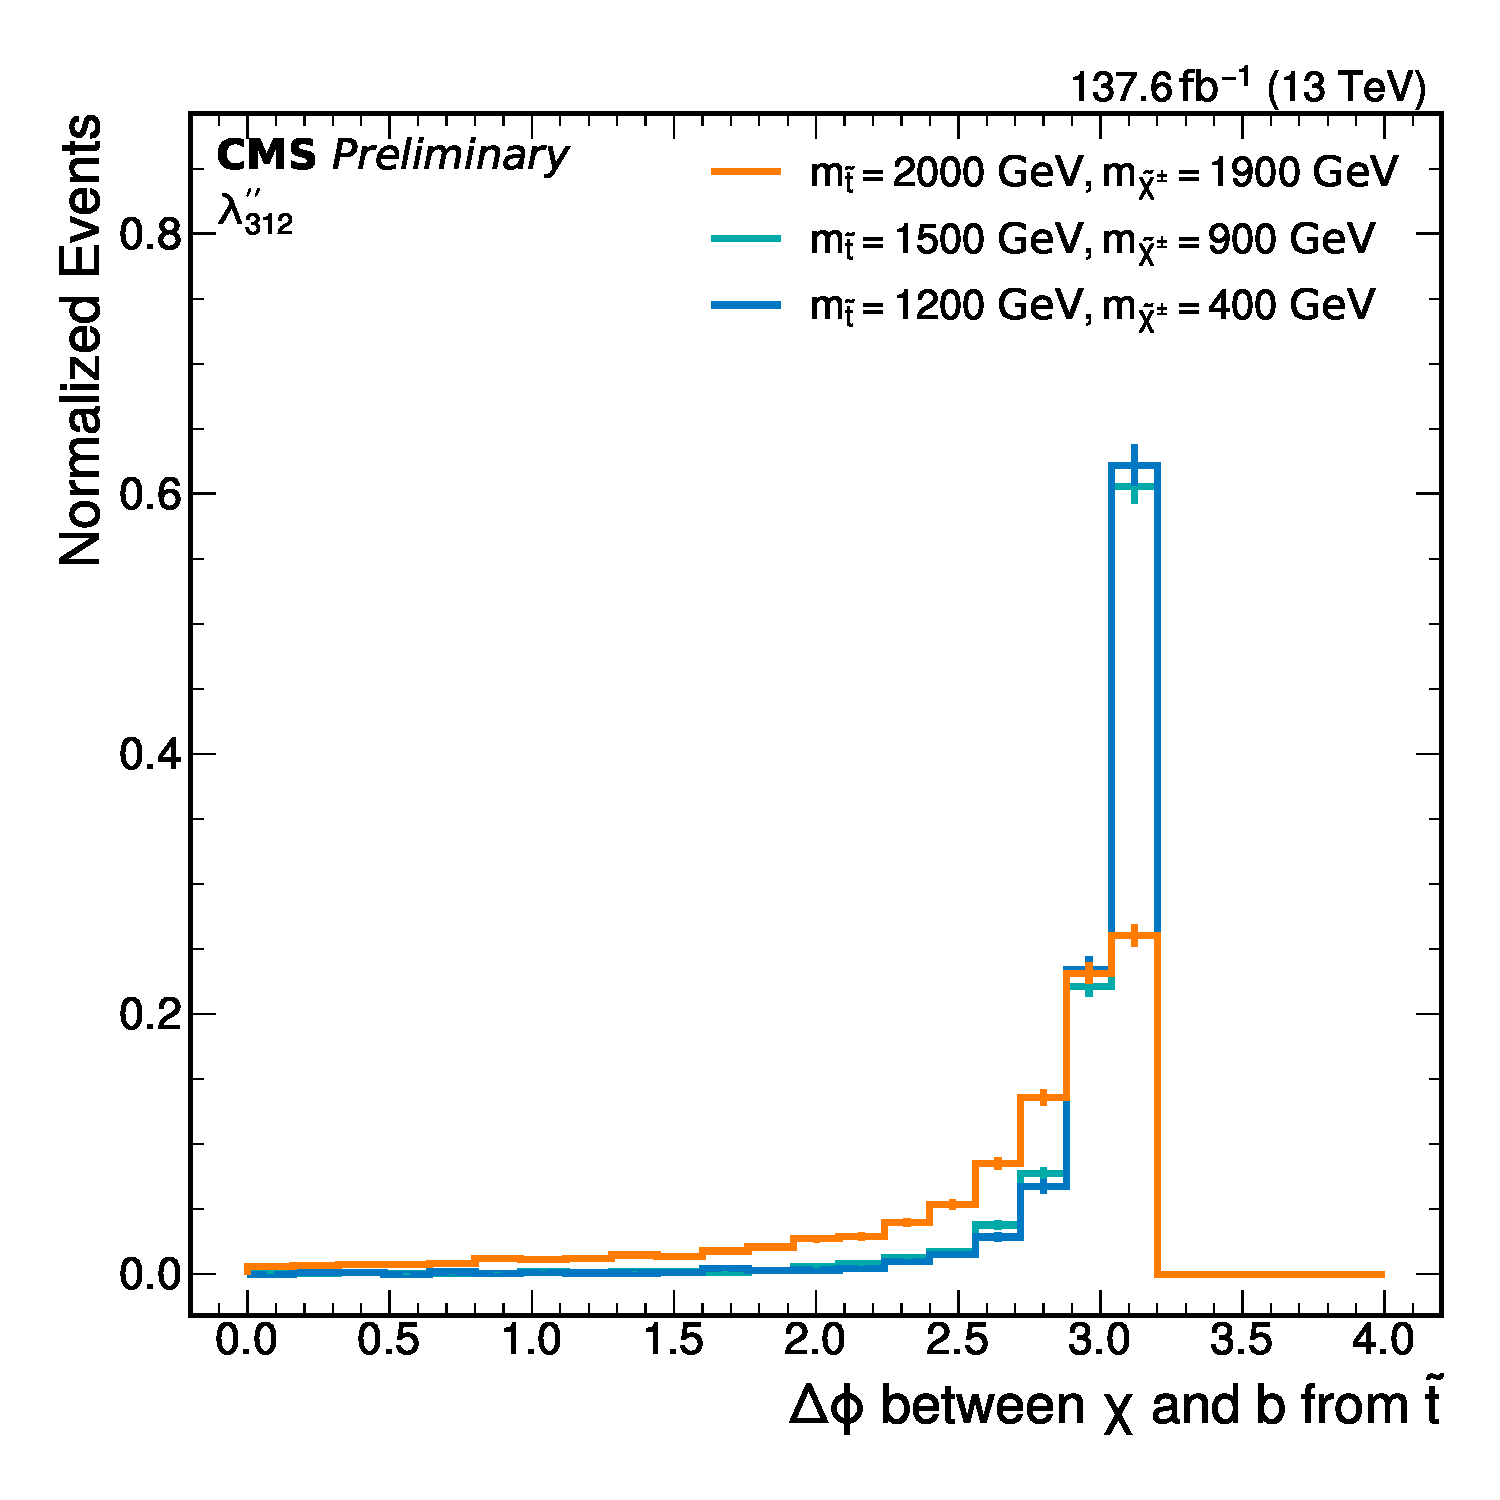
\includegraphics[width=0.3\textwidth]{figures/chi_b_phi.pdf} \end{onlyenv}
      \begin{onlyenv}<4>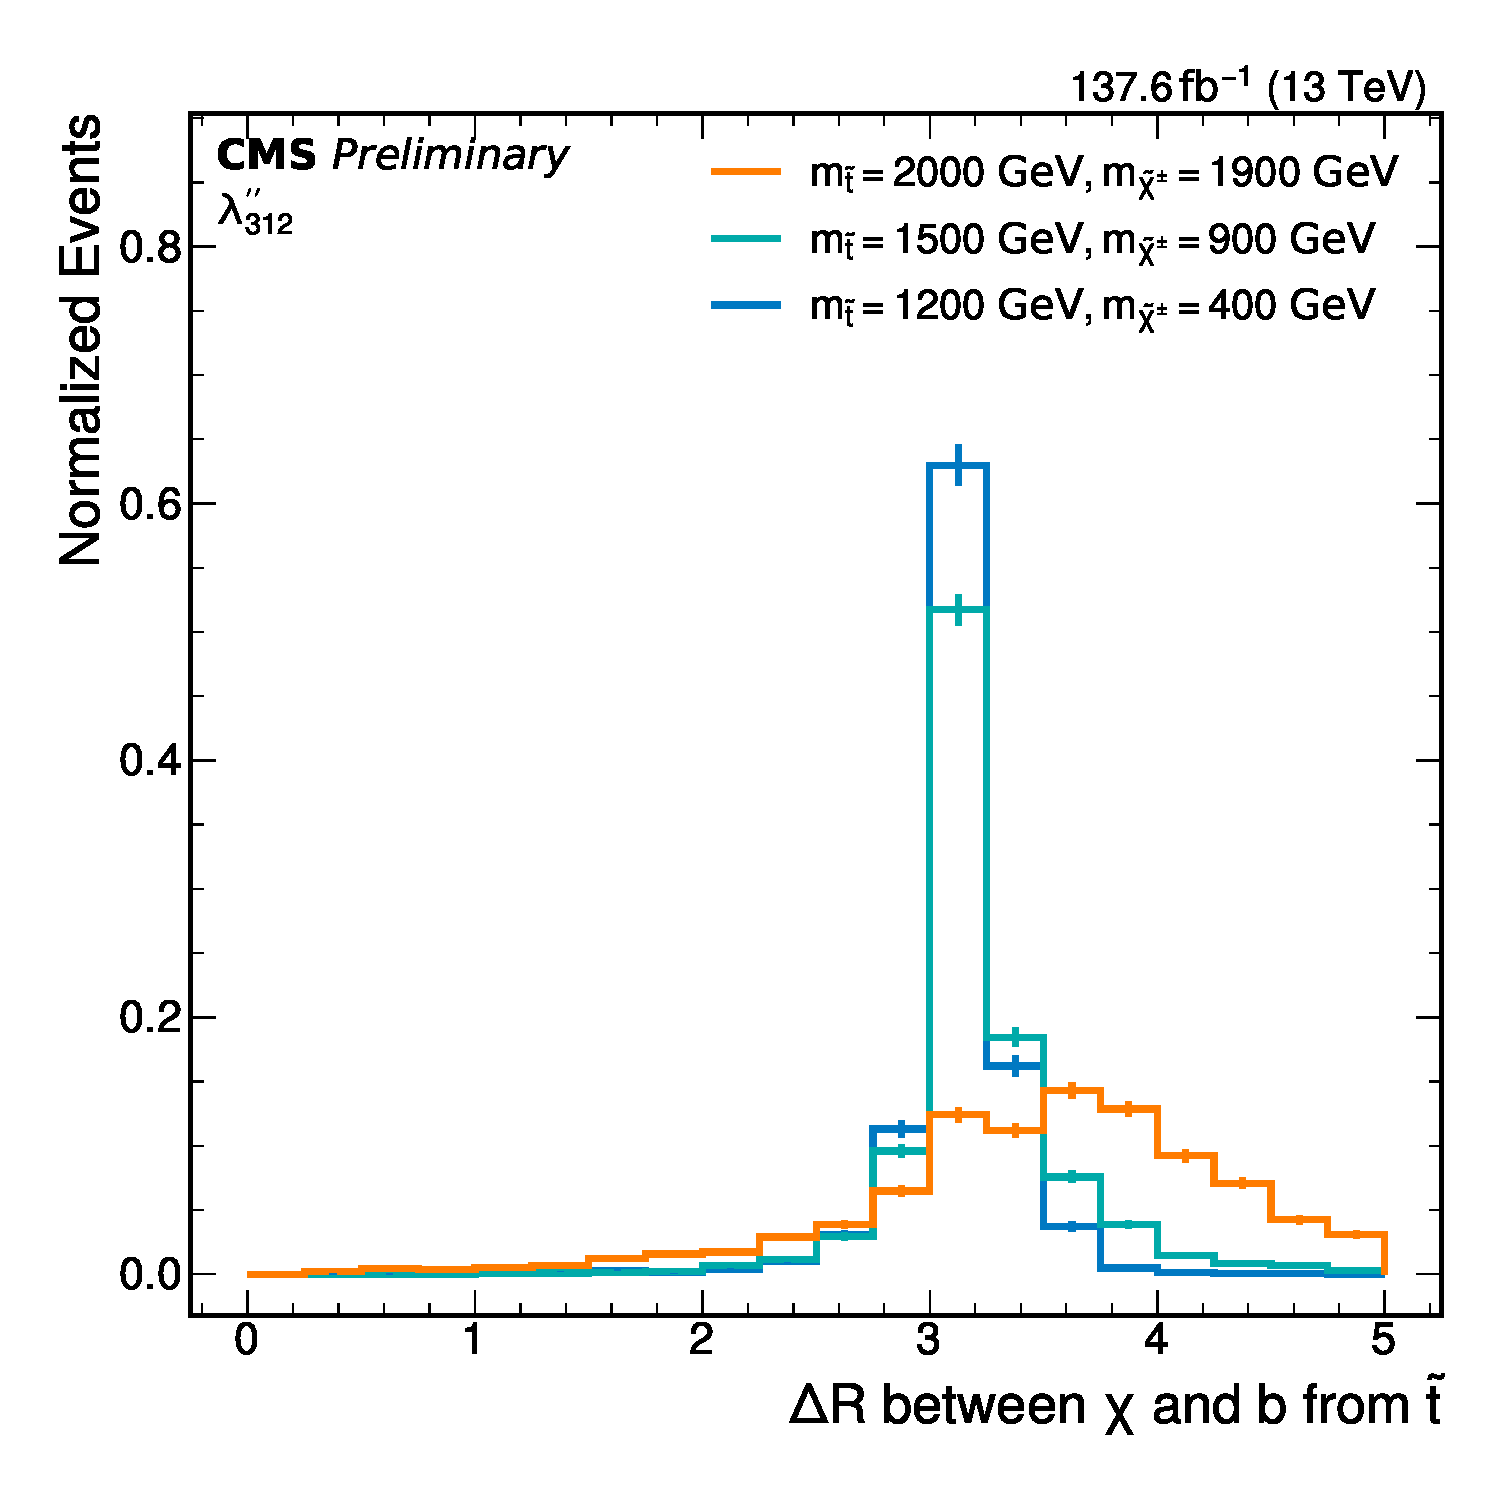
\includegraphics[width=0.3\textwidth]{figures/chi_b_dr.pdf} \end{onlyenv}
      \begin{onlyenv}<5>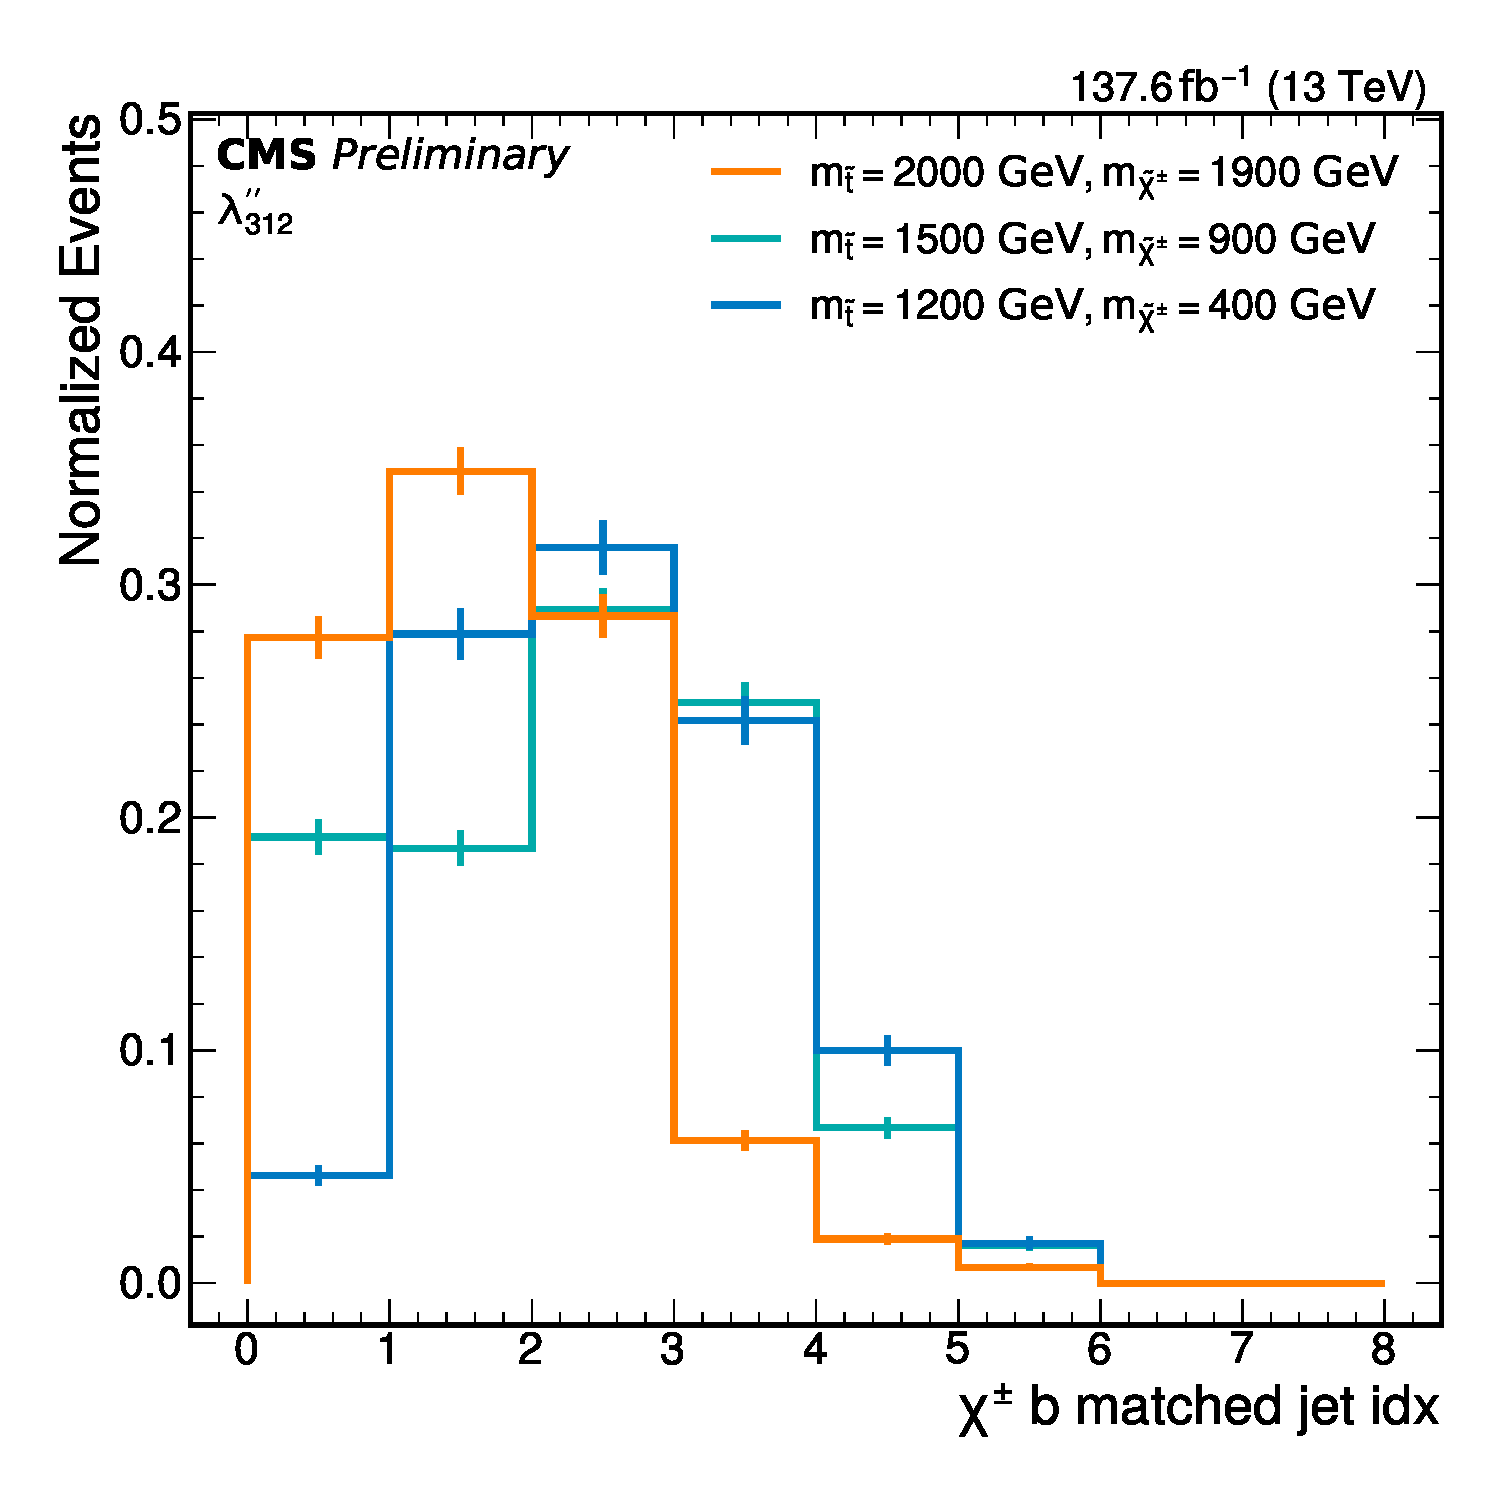
\includegraphics[width=0.4\textwidth]{figures/chi_b_jet_idx.pdf} \end{onlyenv}
      \begin{onlyenv}<5>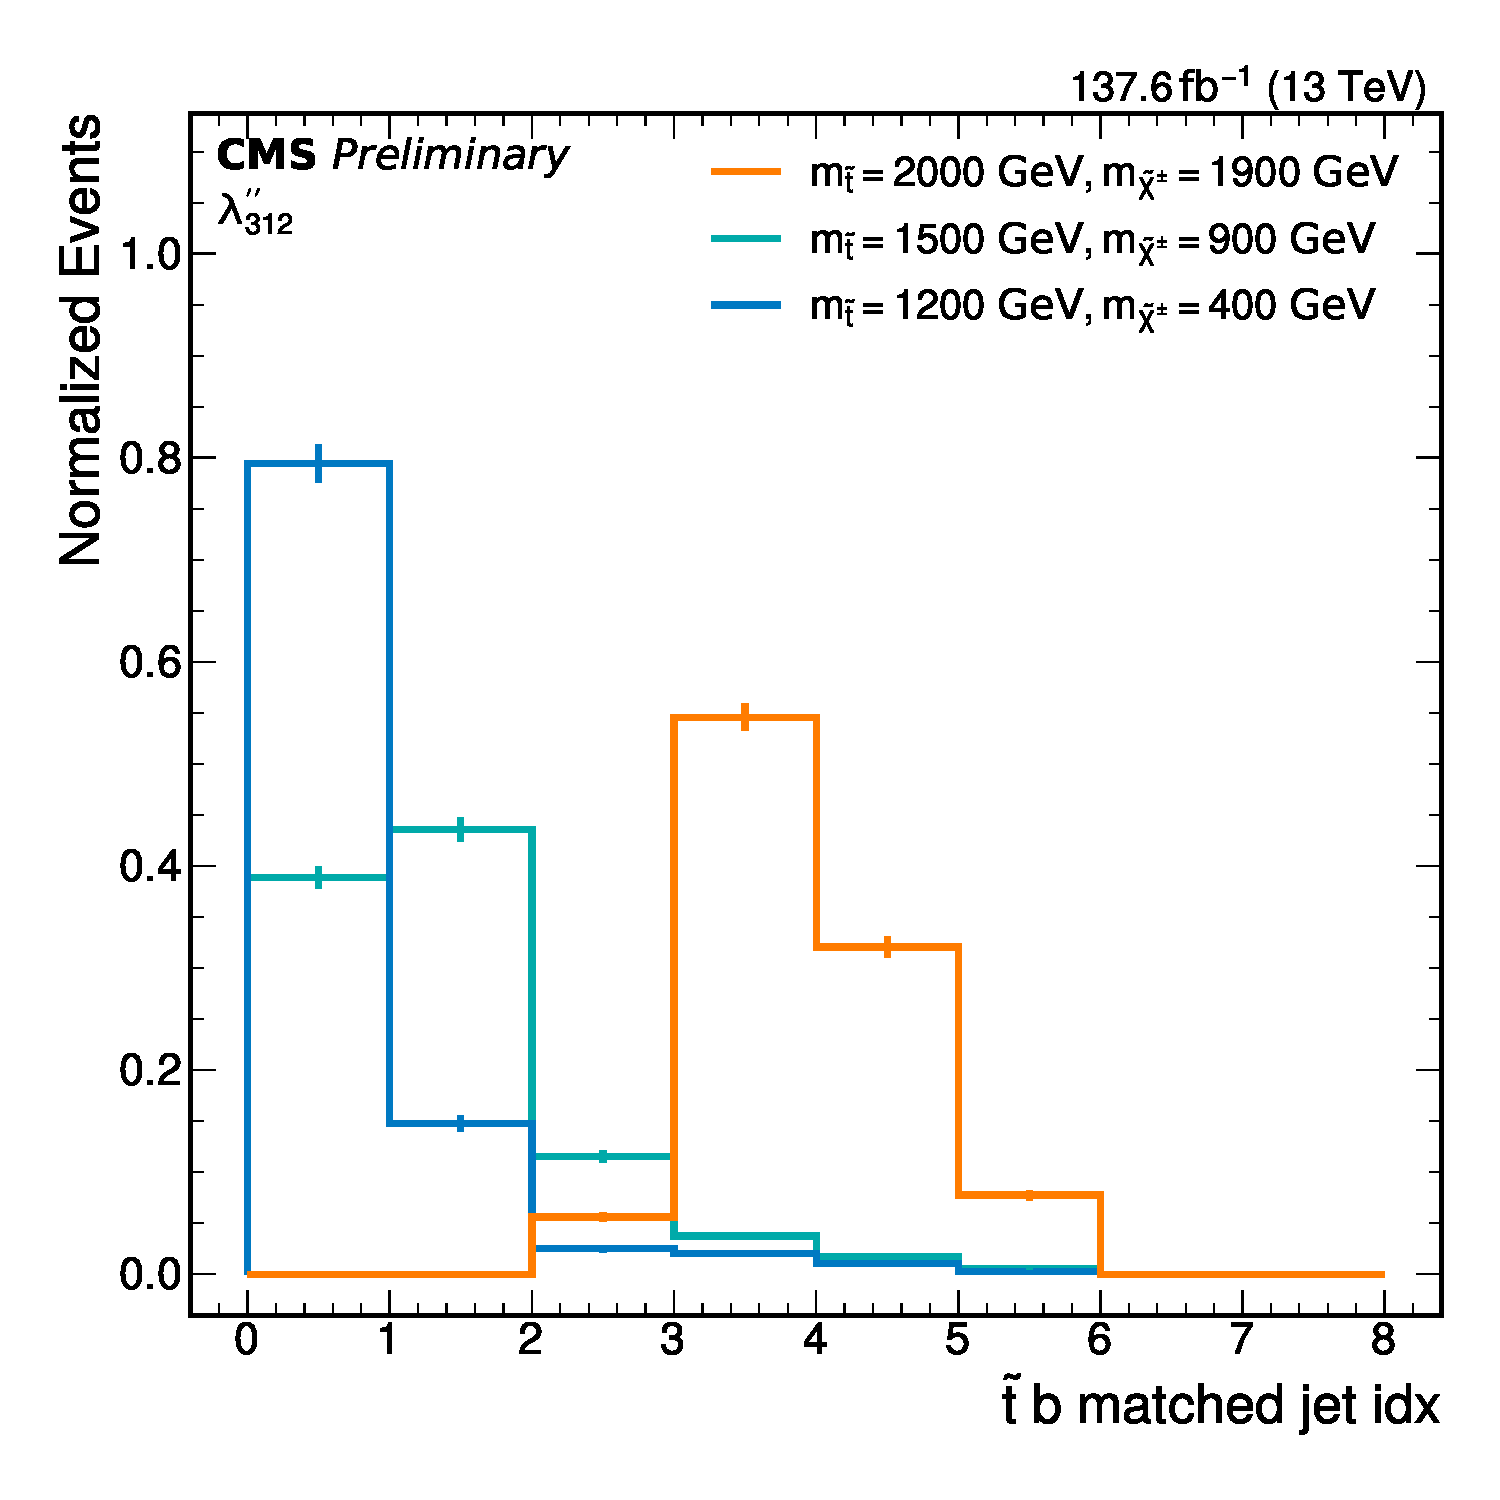
\includegraphics[width=0.4\textwidth]{figures/stop_b_jet_idx.pdf} \end{onlyenv}
    \end{center}
    % \end{overlayarea}
\end{frame}

\section{Event Selection}
\label{sec:event-selection}

\begin{frame}<1,2,3,4>[label=event-characteristics]{Key Event Characteristics}
  \begin{onlyenv}<1>
    \begin{itemize}
    \item No leptons.
    \item A moderate number of jets, several with high $p_{T}$.
    \item Multiple b-jets (jets identified to have come from a \quarkb), and large angular separation between b-jets. 
    \end{itemize}
    {\bfseries     These signatures match most closely with QCD and \quarkt\aquarkt{}}
    \begin{center}
      \scalebox{0.7}{\begin{tikzpicture}
          \drawdiagram{$d_{i}$}{$d_{j}$}
        \end{tikzpicture}}
    \end{center}
  \end{onlyenv}

  \begin{onlyenv}<2-3>
    \begin{itemize}
    \item To further reduce the QCD multijet and \quarkt\aquarkt{} backgrounds we investigate inspecting N-1 plots (make all cuts except for the one in question).
    \end{itemize}
    \begin{center}
      \begin{tikzpicture}
        \node[anchor=south west,inner sep=0] (image) at (0,0) {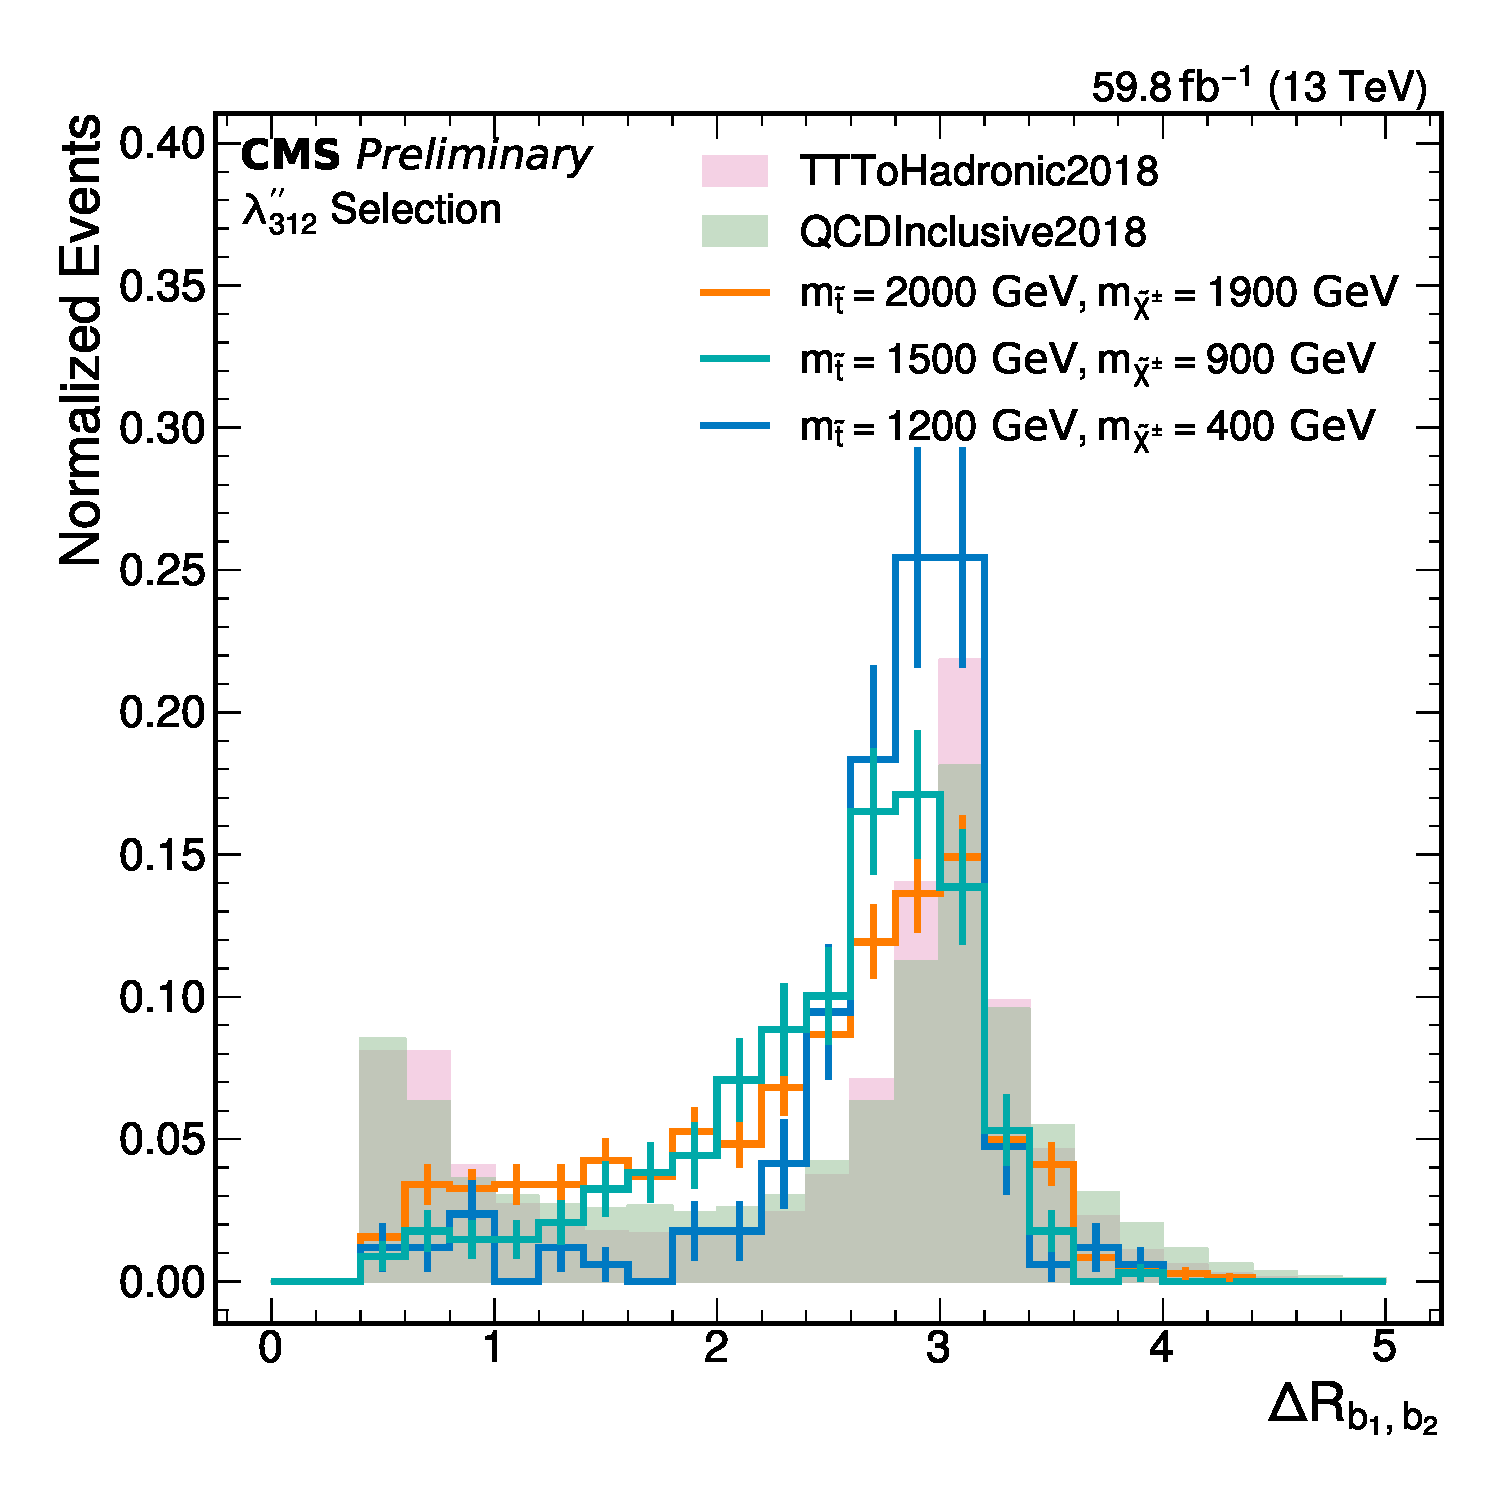
\includegraphics[width=0.3\textwidth]{figures/dRbb12.pdf}};
        \begin{onlyenv}<3>
          \begin{scope}[x={(image.south east)},y={(image.north west)}]
            \coordinate (A) at (0.33,0.12);
            \coordinate (B) at ($(A) + (0,0.7)$);
            \draw[] (A) -- (B);
            \coordinate (C) at ($ (A)!.5!(B) $);
            \coordinate (D) at ($ (C)!1em!-90:(B) $);
            \draw[->] (C) -- (D);
          \end{scope}
        \end{onlyenv}
      \end{tikzpicture}
      \begin{tikzpicture}
        \node[anchor=south west,inner sep=0] (image) at (0,0) {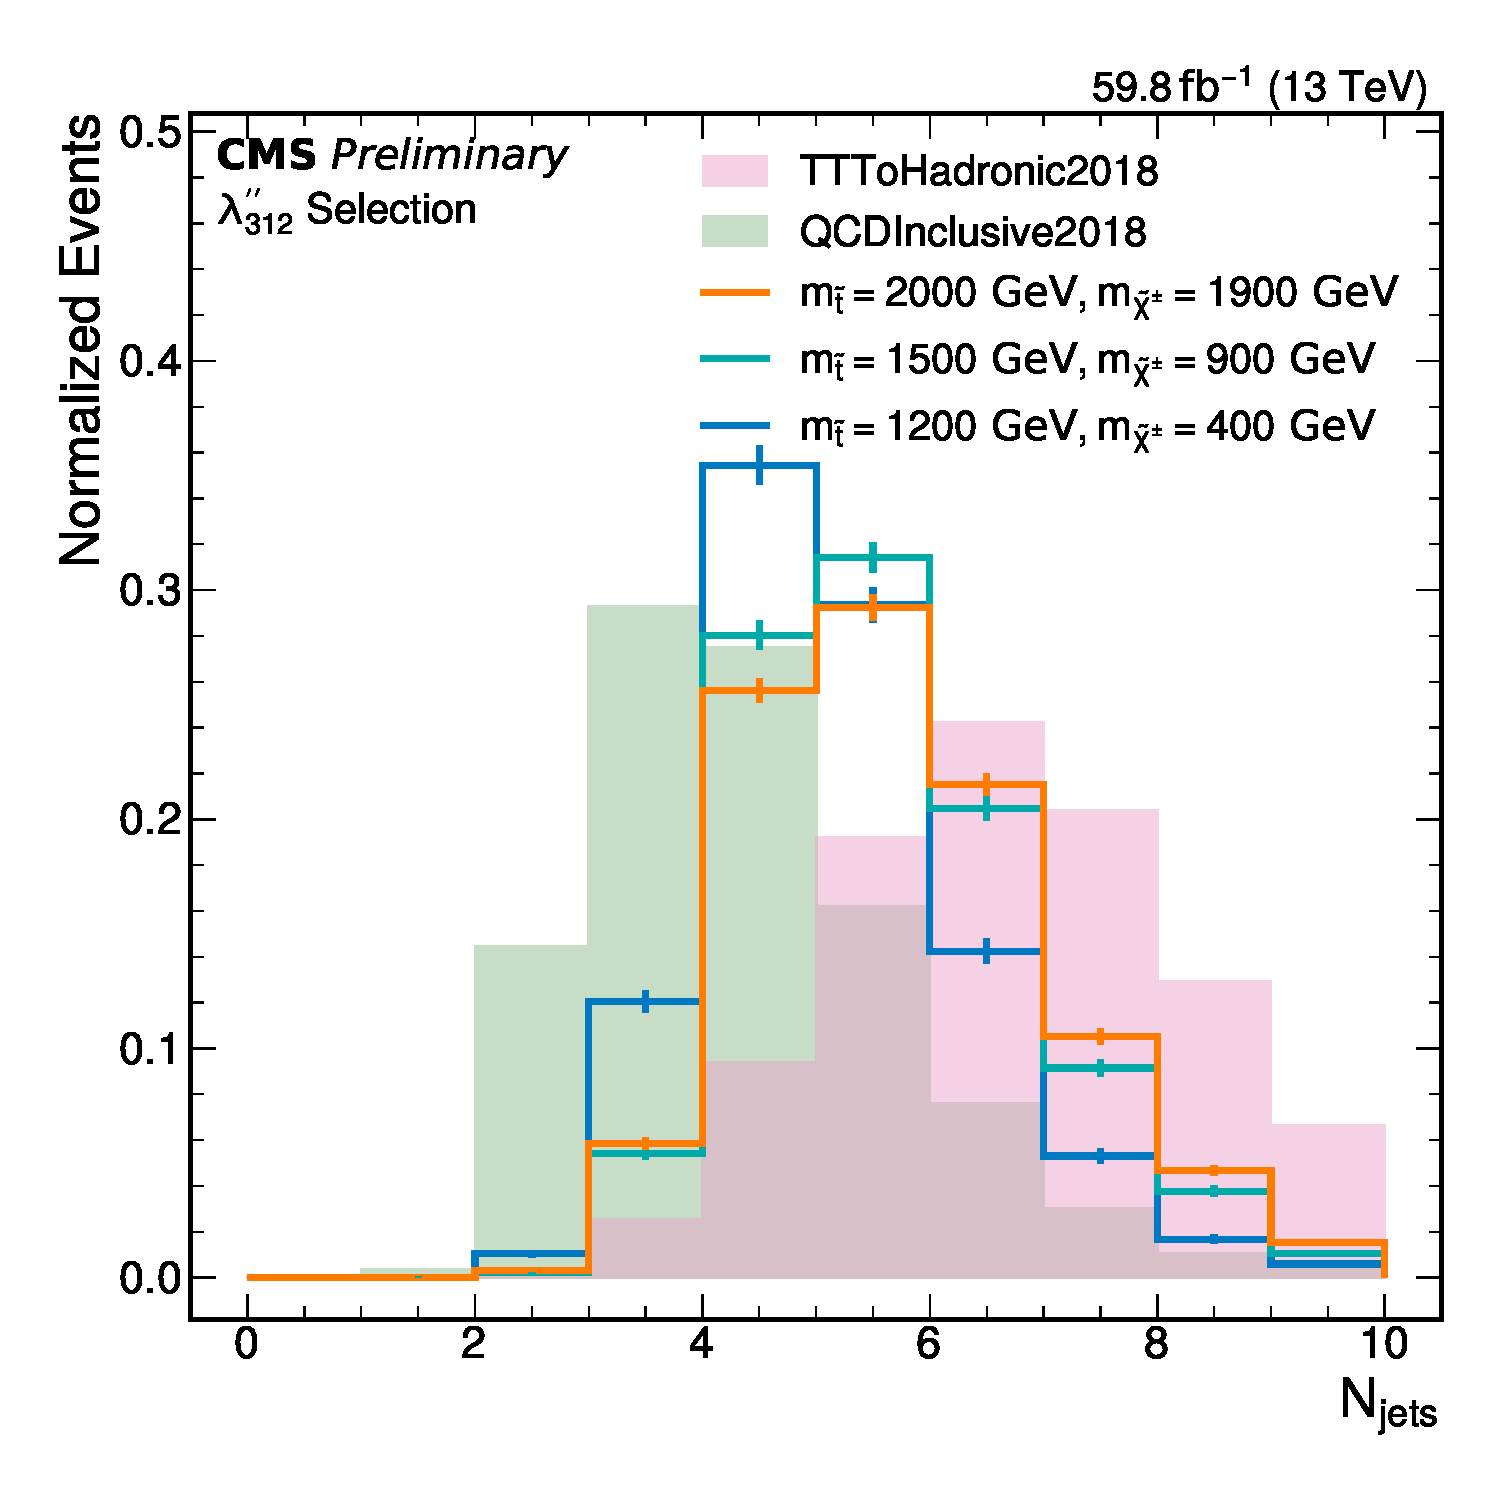
\includegraphics[width=0.3\textwidth]{figures/nJets.pdf}};
        \begin{onlyenv}<3>
          \begin{scope}[x={(image.south east)},y={(image.north west)}]
            \coordinate (A1) at (0.47,0.12);
            \coordinate (B1) at ($(A1) + (0,0.5)$);

            \coordinate (A2) at (0.69,0.12);
            \coordinate (B2) at ($(A2) + (0,0.5)$);
            \draw[] (A1) -- (B1);
            \draw[] (A2) -- (B2);
            \coordinate (C1) at ($ (A1)!.5!(B1) $);
            \coordinate (D1) at ($ (C1)!0.3em!-90:(B1) $);
            \draw[->] (C1) -- (D1);

            \coordinate (C2) at ($ (A2)!.5!(B2) $);
            \coordinate (D2) at ($ (C2)!0.3em!90:(B2) $);
            \draw[->] (C2) -- (D2);
          \end{scope}
        \end{onlyenv}
      \end{tikzpicture}
      \begin{tikzpicture}
        \node[anchor=south west,inner sep=0] (image) at (0,0) {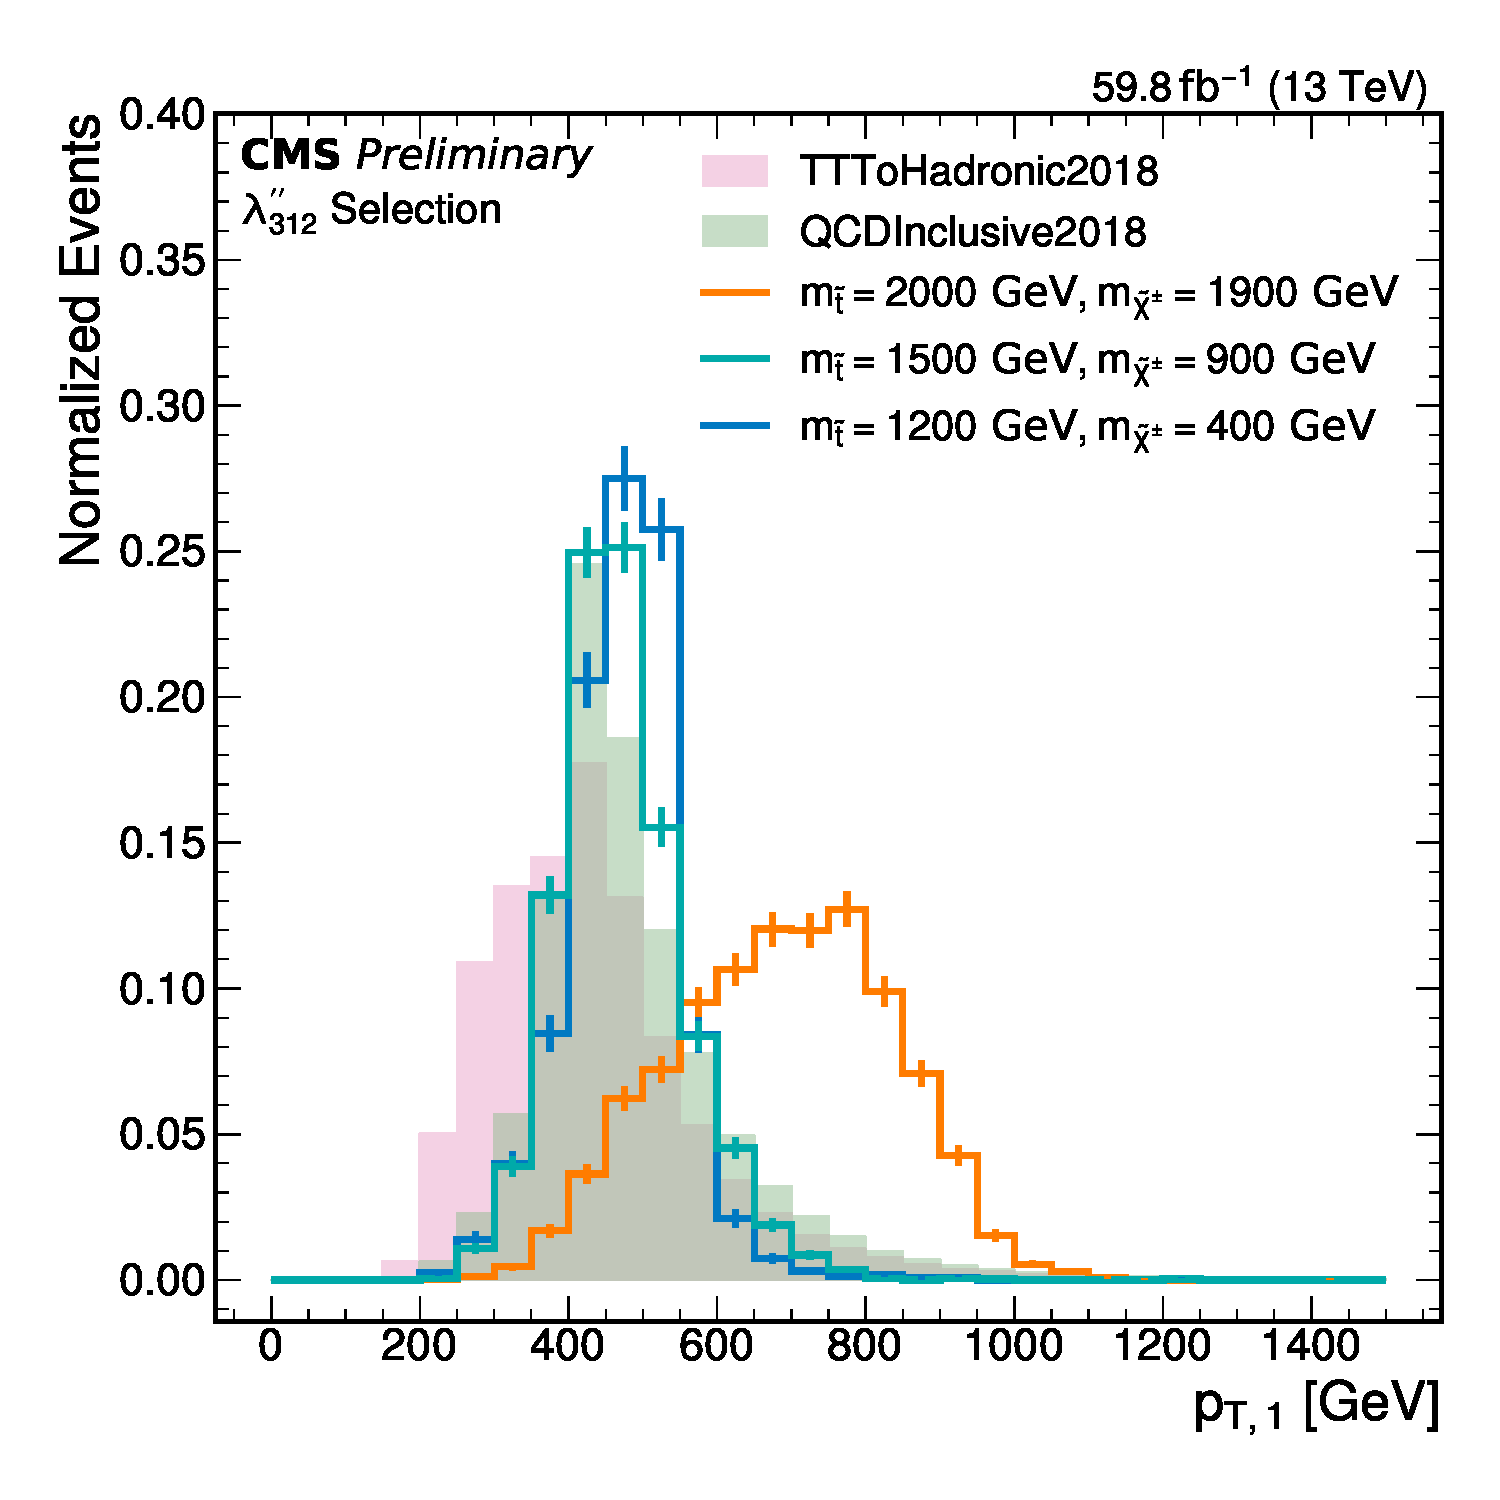
\includegraphics[width=0.3\textwidth]{figures/pT1.pdf}};
        \begin{onlyenv}<3>
          \begin{scope}[x={(image.south east)},y={(image.north west)}]
            \coordinate (A) at (0.33,0.12);
            \coordinate (B) at ($(A) + (0,0.7)$);
            \draw[] (A) -- (B);
            \coordinate (C) at ($ (A)!.5!(B) $);
            \coordinate (D) at ($ (C)!1em!-90:(B) $);
            \draw[->] (C) -- (D);
          \end{scope}
        \end{onlyenv}
      \end{tikzpicture}
    \end{center}
  \end{onlyenv}

  \begin{onlyenv}<4>
    \begin{columns}
      \begin{column}{0.5\textwidth}
        \begin{itemize}
        \item We can make additional cuts to further reduce the QCD and \quarkt\aquarkt{} backgrounds. 
        \item The final signal region selection is shown below. 
        \end{itemize}
      \end{column}
      \begin{column}{0.5\textwidth}
        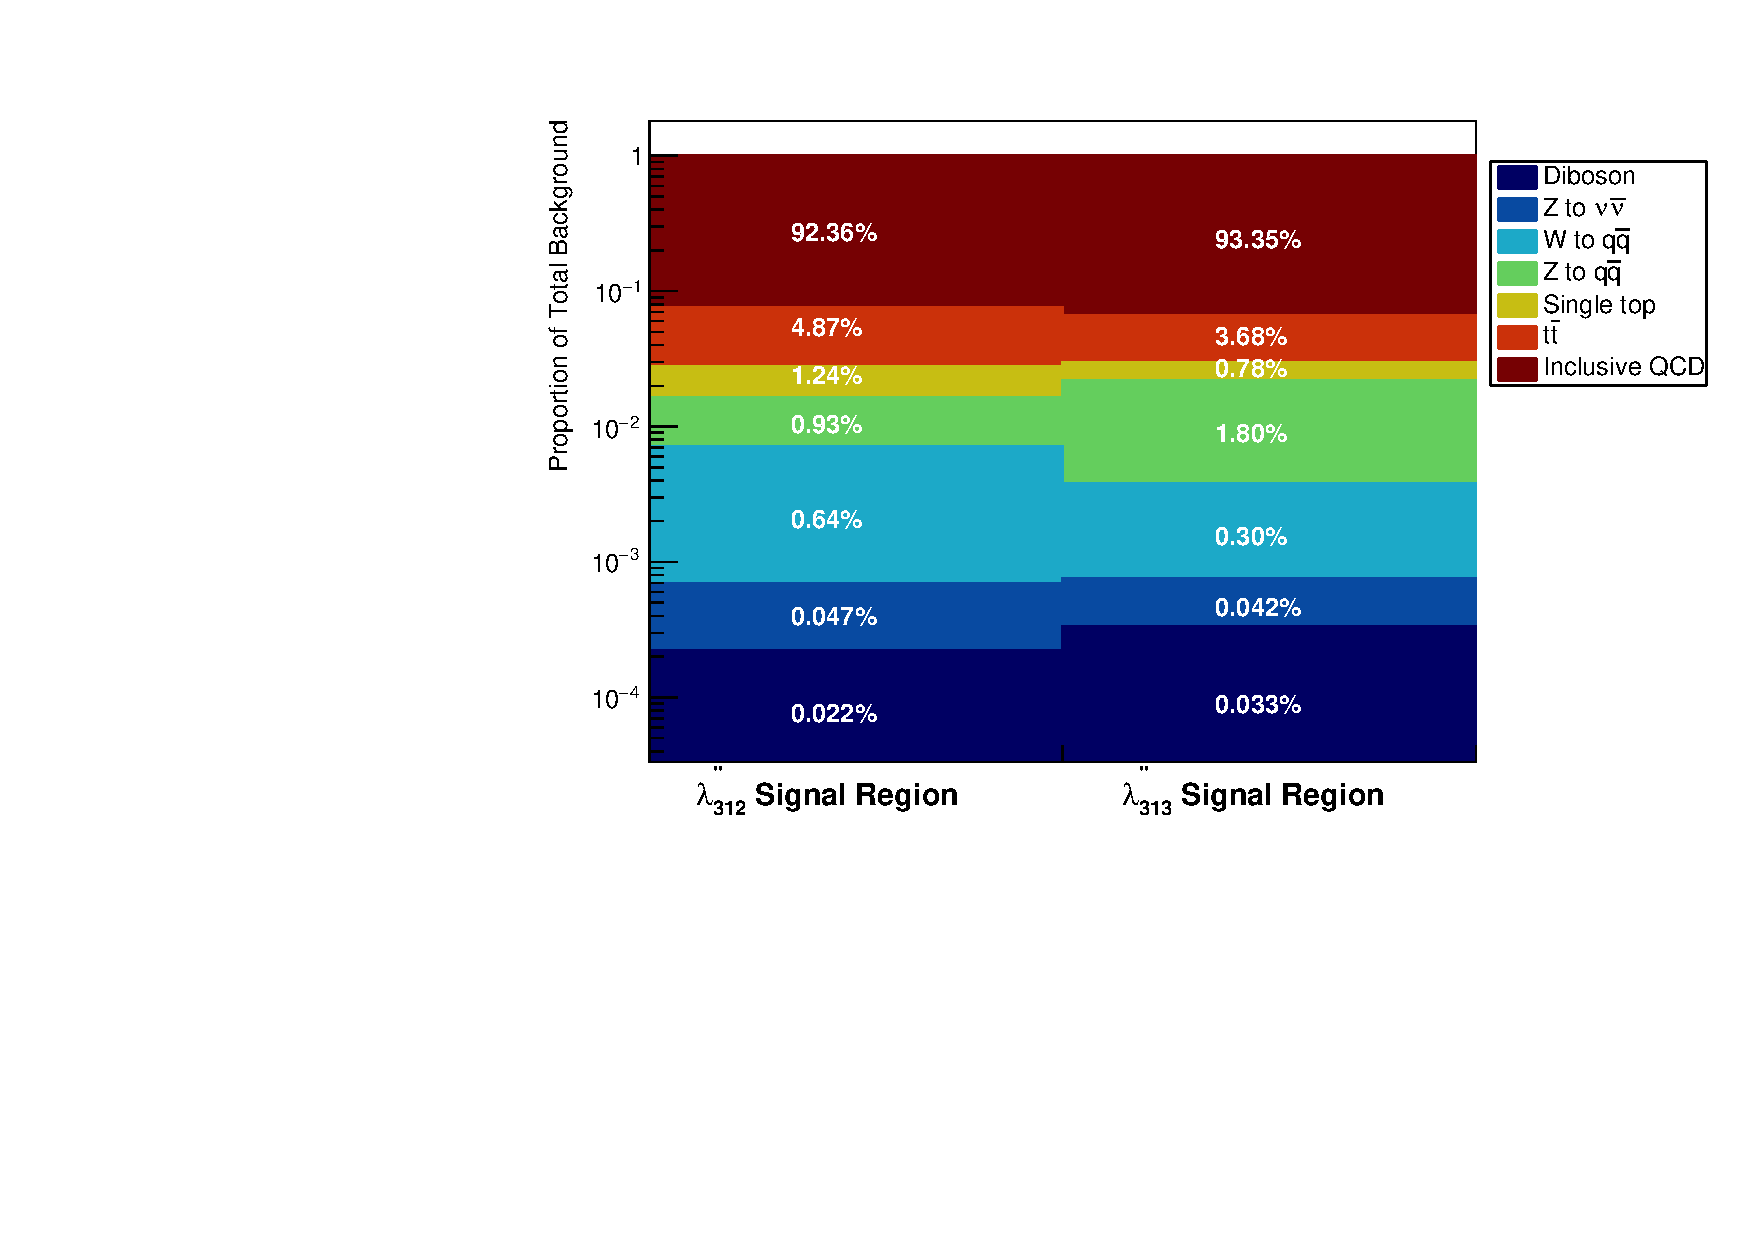
\includegraphics[width=\textwidth]{figures/backgroundStack.pdf}
      \end{column}
    \end{columns}

    \begin{columns}
      \begin{column}{\textwidth}
        \begin{center}
          \scalebox{0.6}{
            \begin{tabular}{|cccc|}
              \hline
              \multicolumn{4}{|c|}{Baseline Selections} \\ \hline
              % \multicolumn{4}{|c|}{\texttt{HLT\_PFHT1050 | HLT\_AK8PFJet400\_TrimMass30}} \\
              \multicolumn{4}{|c|}{$4 \leq \mathrm{N_j} \leq 6$ ($p_{\mathrm{T,j}} > 30~\GeV$, $|\eta_{\mathrm{j}}| < 2.4$)} \\
              \multicolumn{4}{|c|}{$p_{\mathrm{T,j_1}} > 300~\GeV$} \\
              \multicolumn{4}{|c|}{$\mathrm{N}_e , \mathrm{N}_\mu  = 0$} \\
              \multicolumn{4}{|c|}{$\Delta R_{\mathrm{b_1,b_2}} > 1$ } \\ 
              \multicolumn{4}{|c|}{$m_4 \equiv m_{\mathrm{j_1,j_2,j_3,j_4}}$} \\ \hline
              \multicolumn{1}{|c|}{\begin{tabular}[c]{@{}c@{}}\coupling{312}\\ Uncompressed SR\end{tabular}} & \multicolumn{1}{c|}{\begin{tabular}[c]{@{}c@{}}\coupling{312}\\ Compressed SR\end{tabular}} & \multicolumn{1}{c|}{\begin{tabular}[c]{@{}c@{}}\coupling{313}\\ Uncompressed SR\end{tabular}} & \begin{tabular}[c]{@{}c@{}}\coupling{313}\\ Compressed SR\end{tabular} \\ \hline
              \multicolumn{1}{|c|}{$\mathrm{N_b } \geq 2$} & \multicolumn{1}{c|}{$\mathrm{N_b } \geq 2$} & \multicolumn{1}{c|}{$\mathrm{N_b } \geq 3$} & \multicolumn{1}{c|}{$\mathrm{N_b} \geq 3$} \\
              \multicolumn{1}{|c|}{$m_3 \equiv m_{\mathrm{j_2,j_3,j_4}}$} & \multicolumn{1}{c|}{$m_3 \equiv m_{\mathrm{j_1,j_2,j_3}}$} & \multicolumn{1}{c|}{$m_3 \equiv m_{\mathrm{j_2,j_3,j_4}}$} & $m_3 \equiv m_{\mathrm{j_1,j_2,j_3}}$ \\ \hline
            \end{tabular}
          }
\end{center}
        \end{column}
      \end{columns}
  \end{onlyenv}
\end{frame}

\section{Analysis Strategy}
\label{sec:analysis-strat}

\begin{frame}{Strategy Overview}
  \begin{enumerate}
  \item Reconstruct the signal resonances for \textcolor{blue}{\stopq{}} and \textcolor{red}{\chargino{}}.
  \item Estimate the SM background.
  \item Perform a one or two dimensional bump hunt for these resonances. 
  \end{enumerate}
  \begin{center}
    \begin{tikzpicture}[every node/.style={node distance=1cm}]
      \drawdiagram{$d_{i}$}{$d_{j}$}
      \node[ellipse, rotate fit=10, draw=red,inner sep=0pt,fit=(xb) (xs) (xd)] {};
      \node[ellipse, rotate fit=20, draw=blue,inner sep=0pt,fit=(stopb) (xb) (xs) (xd)] {};
    \end{tikzpicture}
  \end{center}
\end{frame}

\begin{frame}<1,2>[label=mass-reconstruction]{Mass Reconstruction}
  \begin{overlayarea}{\textwidth}{3.5cm}
    \begin{itemize}
    \item Resonant masses can be reconstructed using the invariant mass of a well chosen set of jets. 
    \item<only@1> Simplest Reconstruction:
      \begin{itemize}
      \item $m_{\stopq} = m \left( j_1 + j_2 + j_3 + j_4 \right)$ 
      \item Compressed: $m_{\chargino} = m \left( j_1 + j_2 + j_3 \right)$ 
      \item Uncompressed: $m_{\chargino} = m \left( j_2 + j_3 + j_4 \right)$ 
      \end{itemize}
    \item<only@2> Different categories need different treatment
      \begin{itemize}
      \item<only@2-> For both the \stopq{} and compressed \chargino{}, the simplest algorithm works reasonably well. 
      \item<only@2> For the uncompressed \chargino{}, the naive estimation is quite poor.
      \end{itemize}
    \item<only@3-> We can make a simple improvement by requiring the highest \pt{} b-jet used for the \stopq{} but not the \chargino{}.
    \item<only@2,3-> Ongoing work: We can take advantage of both flavor and kinematic information to improve our reconstruction.
    \end{itemize}
  \end{overlayarea}
  \begin{center}
    \begin{columns}
      \begin{column}{0.32\textwidth}
        \onslide<1->{\centering All}

        \includegraphics<1,4>[width=\textwidth]{figures/all_m14_m.pdf} 
        \includegraphics<2->[width=\textwidth]{figures/num_top_4_jets_matched_stop_children.pdf}
      \end{column}
      \begin{column}{0.32\textwidth}
        \onslide<1->{\centering Compressed}

        \includegraphics<1,4>[width=\textwidth]{figures/m13_m.pdf}
        \includegraphics<2->[width=\textwidth]{figures/m13_matching_all_three.pdf}
      \end{column}
      \begin{column}{0.32\textwidth}
        \onslide<1->{\centering Uncompressed}

        \includegraphics<1>[width=\textwidth]{figures/m24_m.pdf}
        \includegraphics<2>[width=\textwidth]{figures/m24_matching_all_three.pdf}
        \includegraphics<3>[width=\textwidth]{figures/m3_top_3_no_lead_b_matching_all_three.pdf}
        \includegraphics<4>[width=\textwidth]{figures/m3_top_3_no_lead_b.pdf}
      \end{column}
    \end{columns}
  \end{center}
\end{frame}


\begin{frame}{2D Resonance Fitting}
  \def\thiswidth{1}
  \begin{columns}[t]
    \begin{column}{0.4\textwidth}
      \small
      \begin{itemize}
      \item<1-> There are two resonances that we expect to form a peak over the background.
      \item<1-> In the uncompressed case, since the leading jet is expected to in $m_{\stopq}$ but not $m_{\chargino}$, we can these reconstructed masses to partially decorrelate.
      \item<1-> In the compressed case, a 1D fit is sufficient. 
      \end{itemize}
    \end{column}
    \begin{column}{0.3\textwidth}
        \centering \textbf{Compressed} 
        \vspace*{-\baselineskip}

      %\begin{onlyenv}<1>
      %  \begin{center}
      %    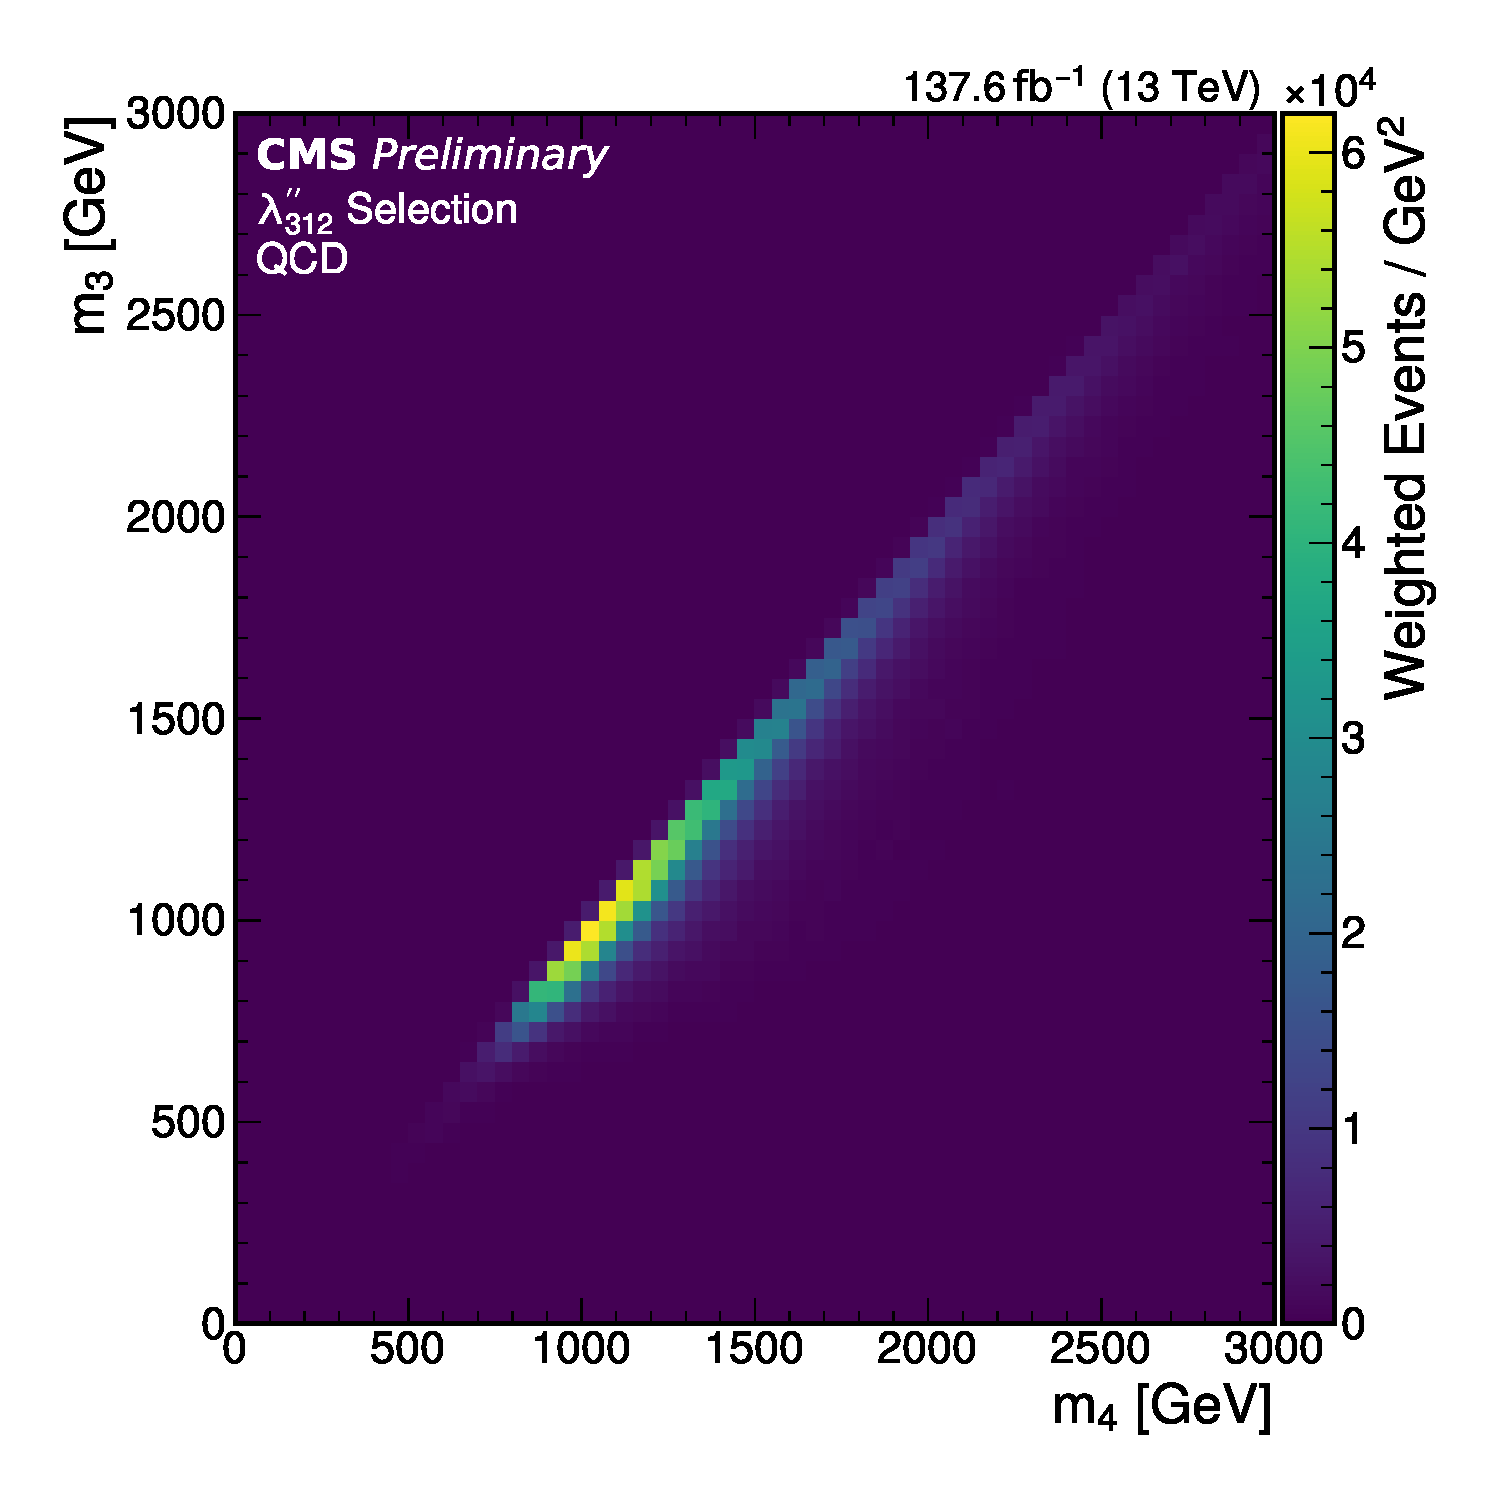
\includegraphics[width=\thiswidth\textwidth]{figures/m14_vs_m13_Skim_QCDInclusive2018.pdf}\\[0em]
      %    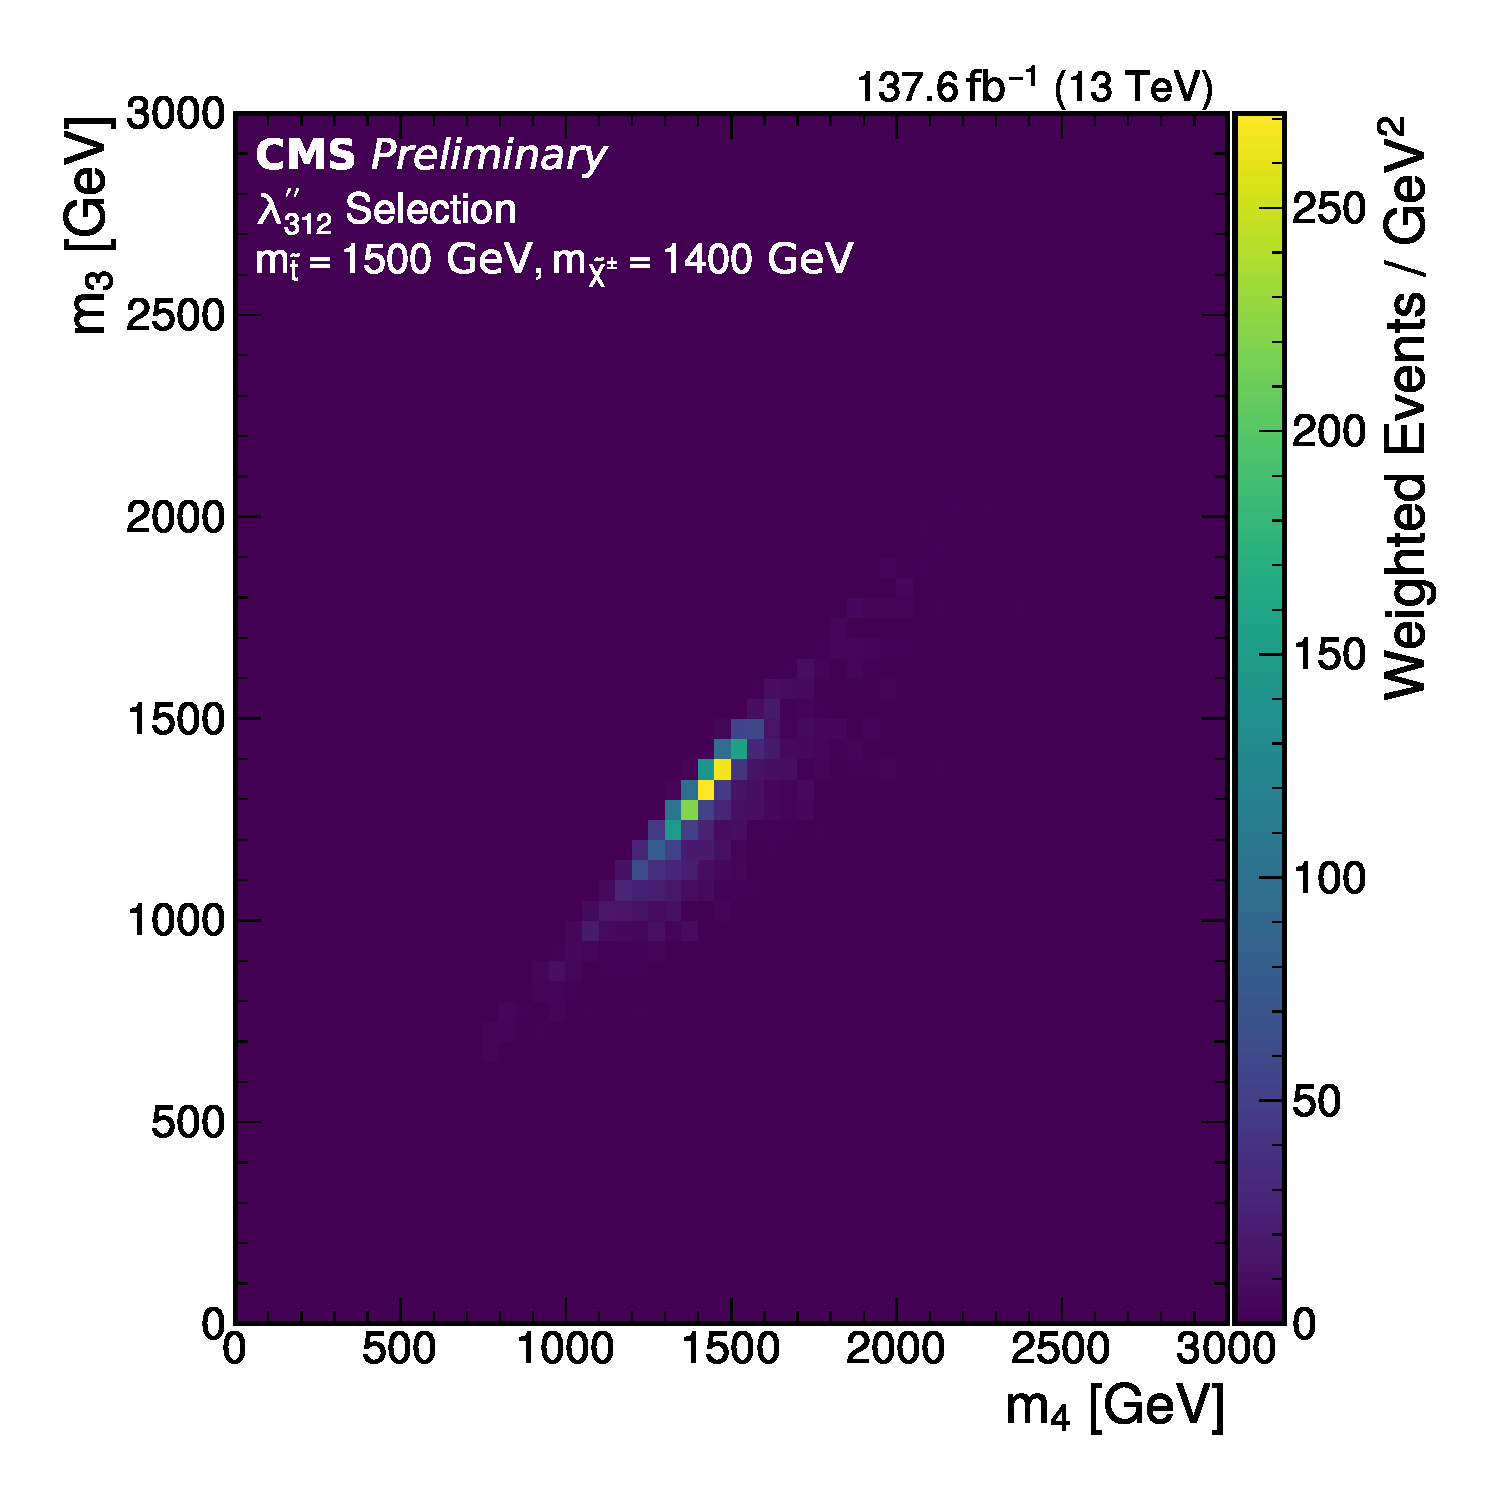
\includegraphics[width=\thiswidth\textwidth]{figures/m14_vs_m13_signal_312_1500_1400.pdf}
      %  \end{center}
      %\end{onlyenv}
      \begin{onlyenv}<1->
        \begin{center}
          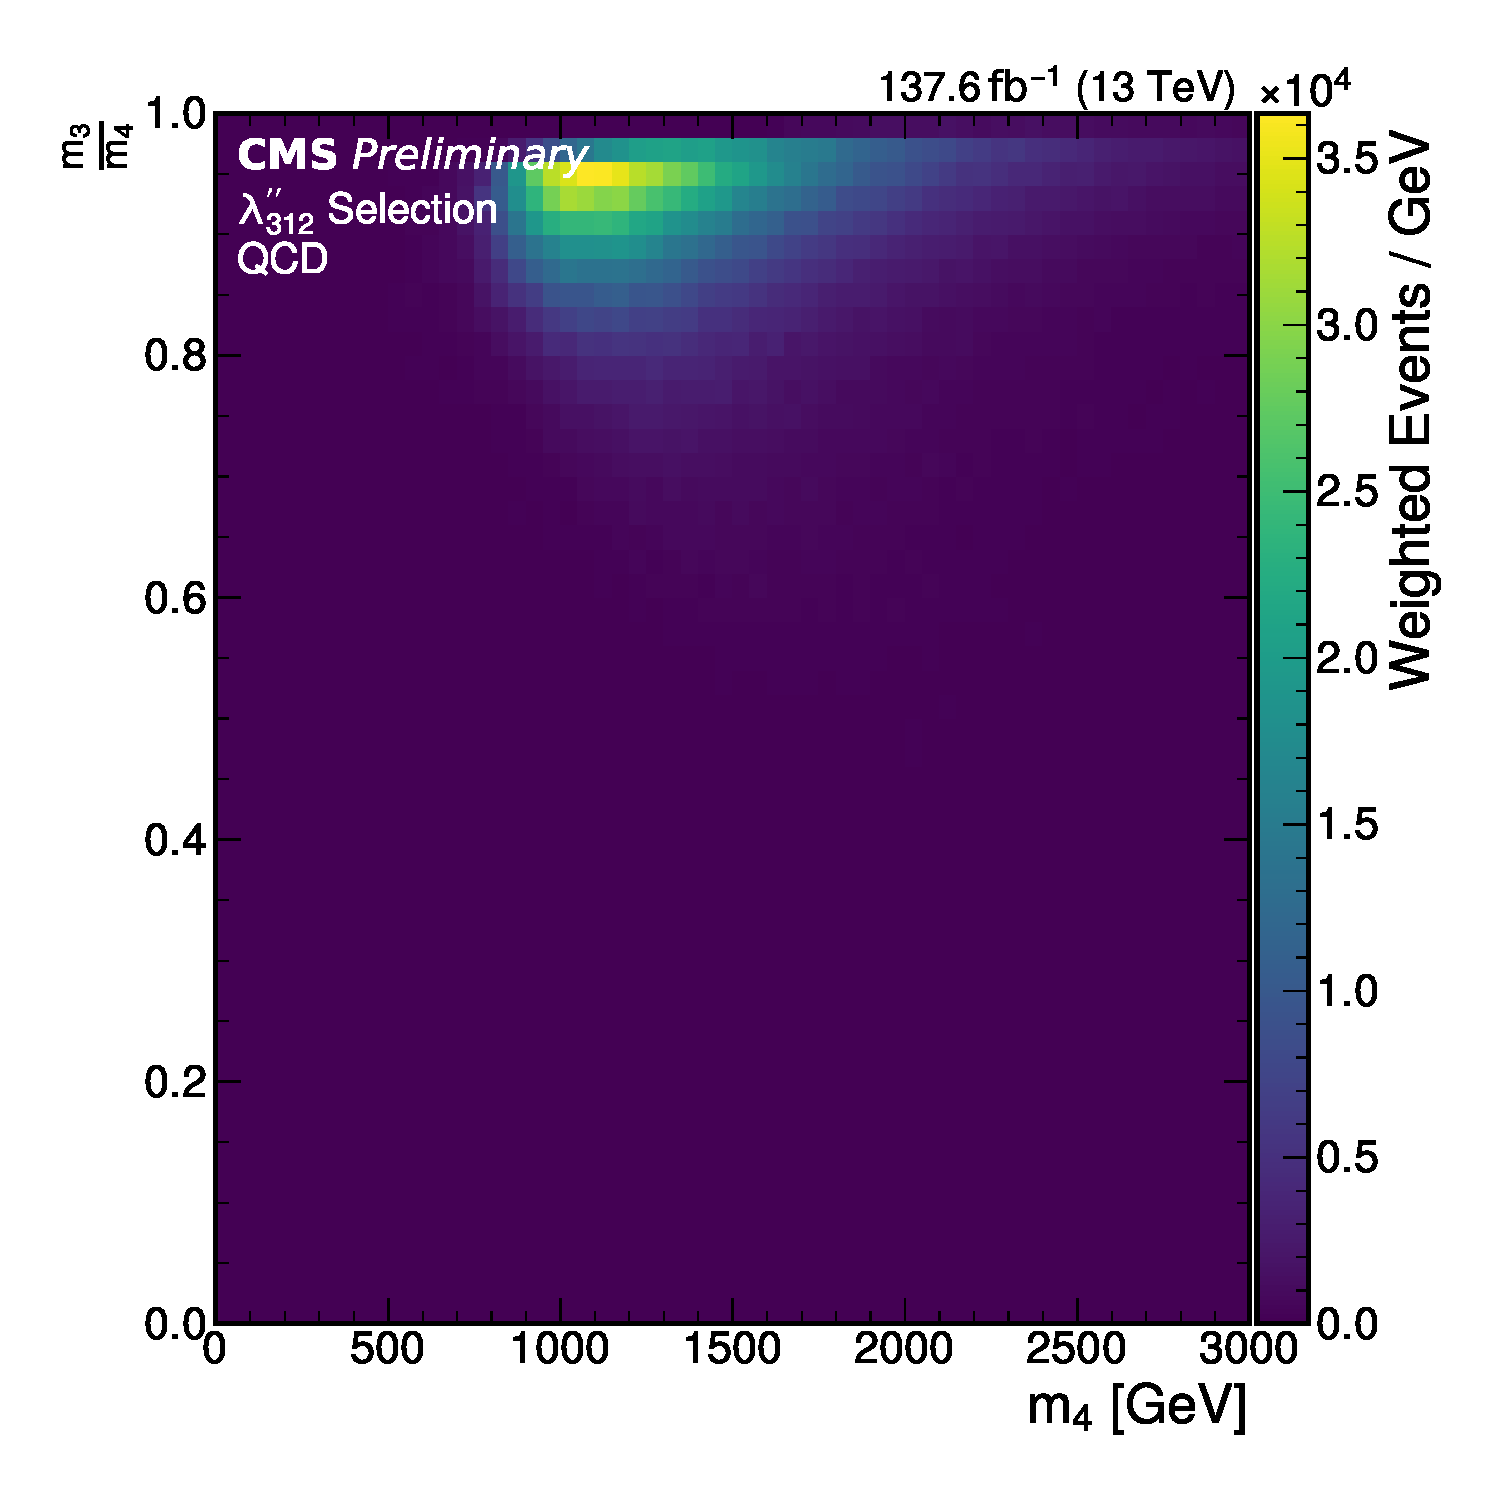
\includegraphics[width=\thiswidth\textwidth]{figures/ratio_m14_vs_m13_Skim_QCDInclusive2018.pdf}\\
          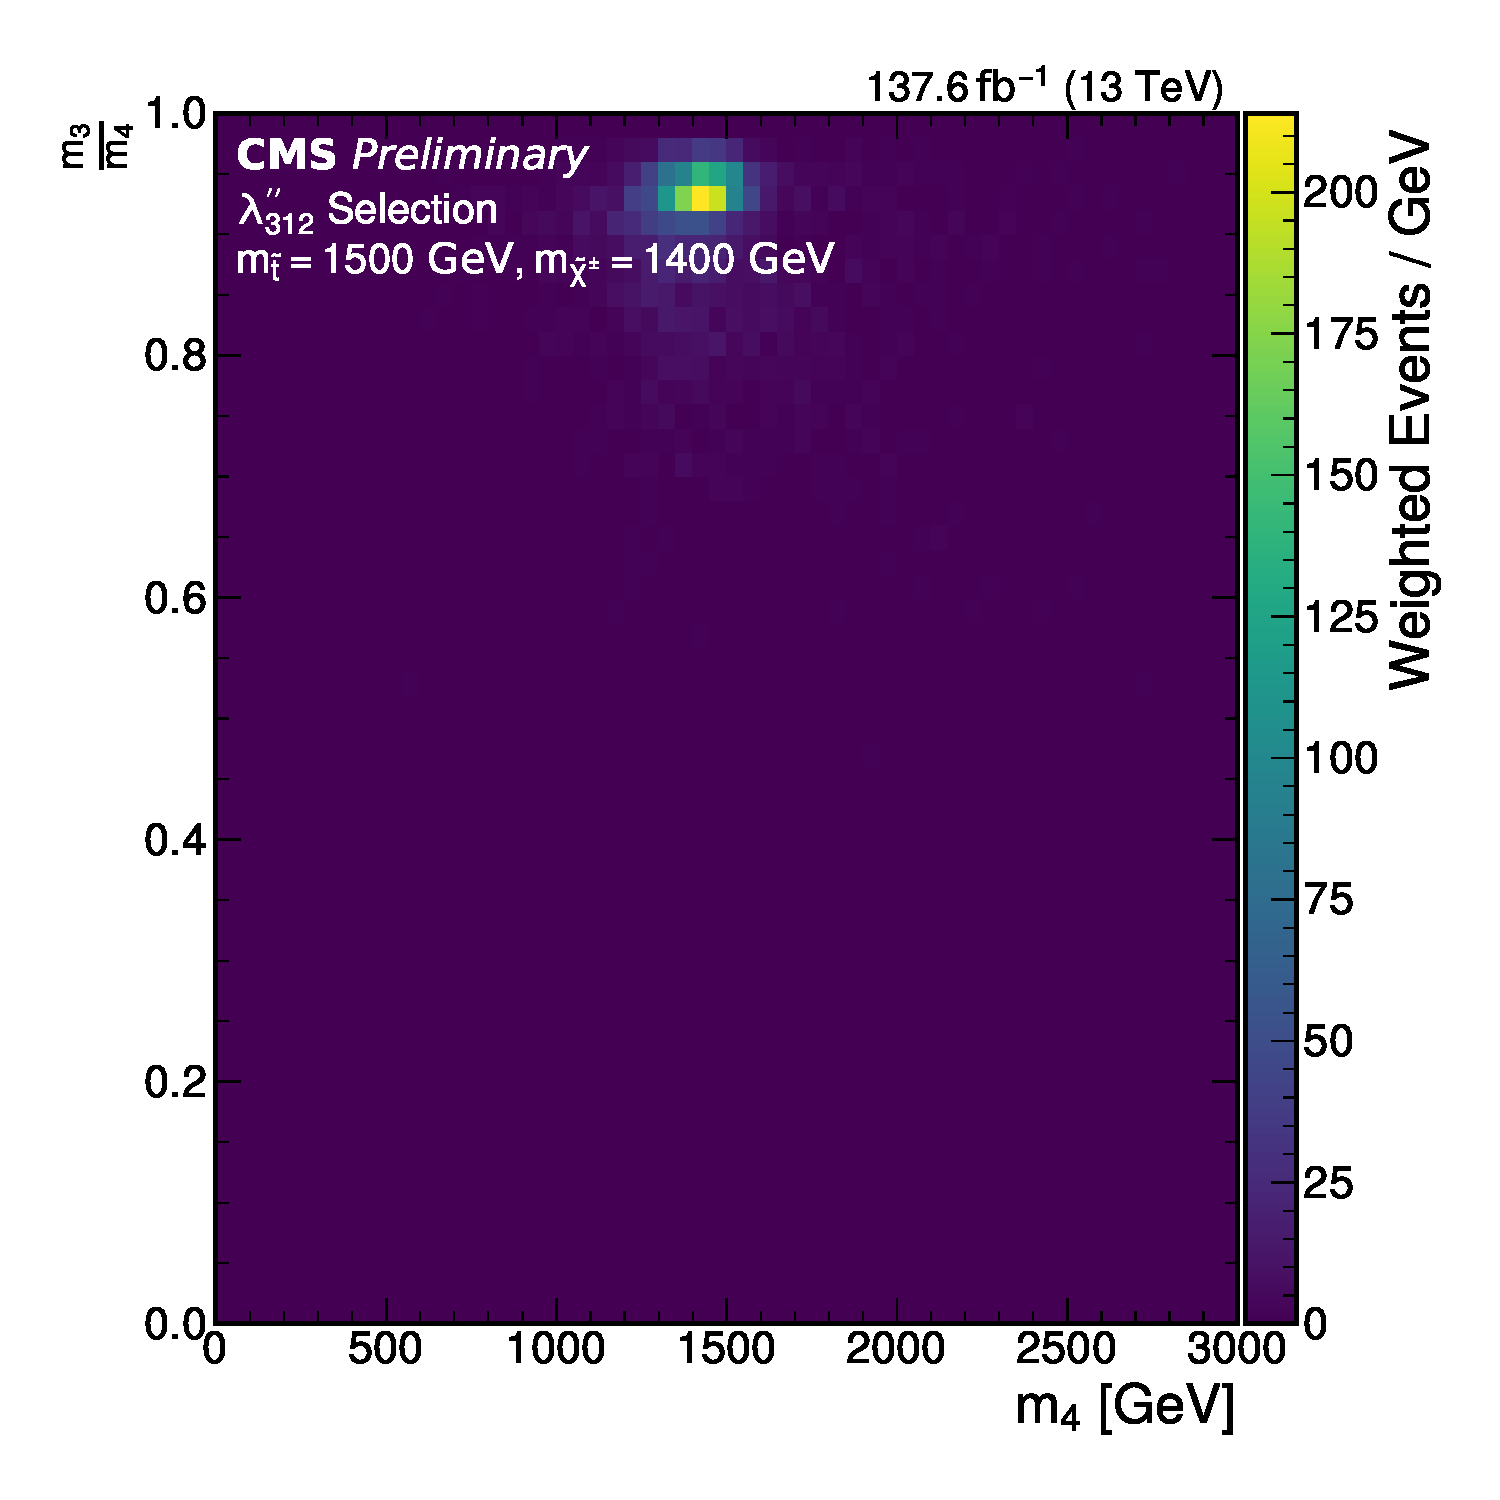
\includegraphics[width=\thiswidth\textwidth]{figures/ratio_m14_vs_m13_signal_312_1500_1400.pdf}
        \end{center}
      \end{onlyenv}
    \end{column}
    \begin{column}{0.3\textwidth}
       \centering \textbf{Uncompressed} 
        \vspace*{-\baselineskip}

     % \begin{onlyenv}<1>
     %   \begin{center}
     %     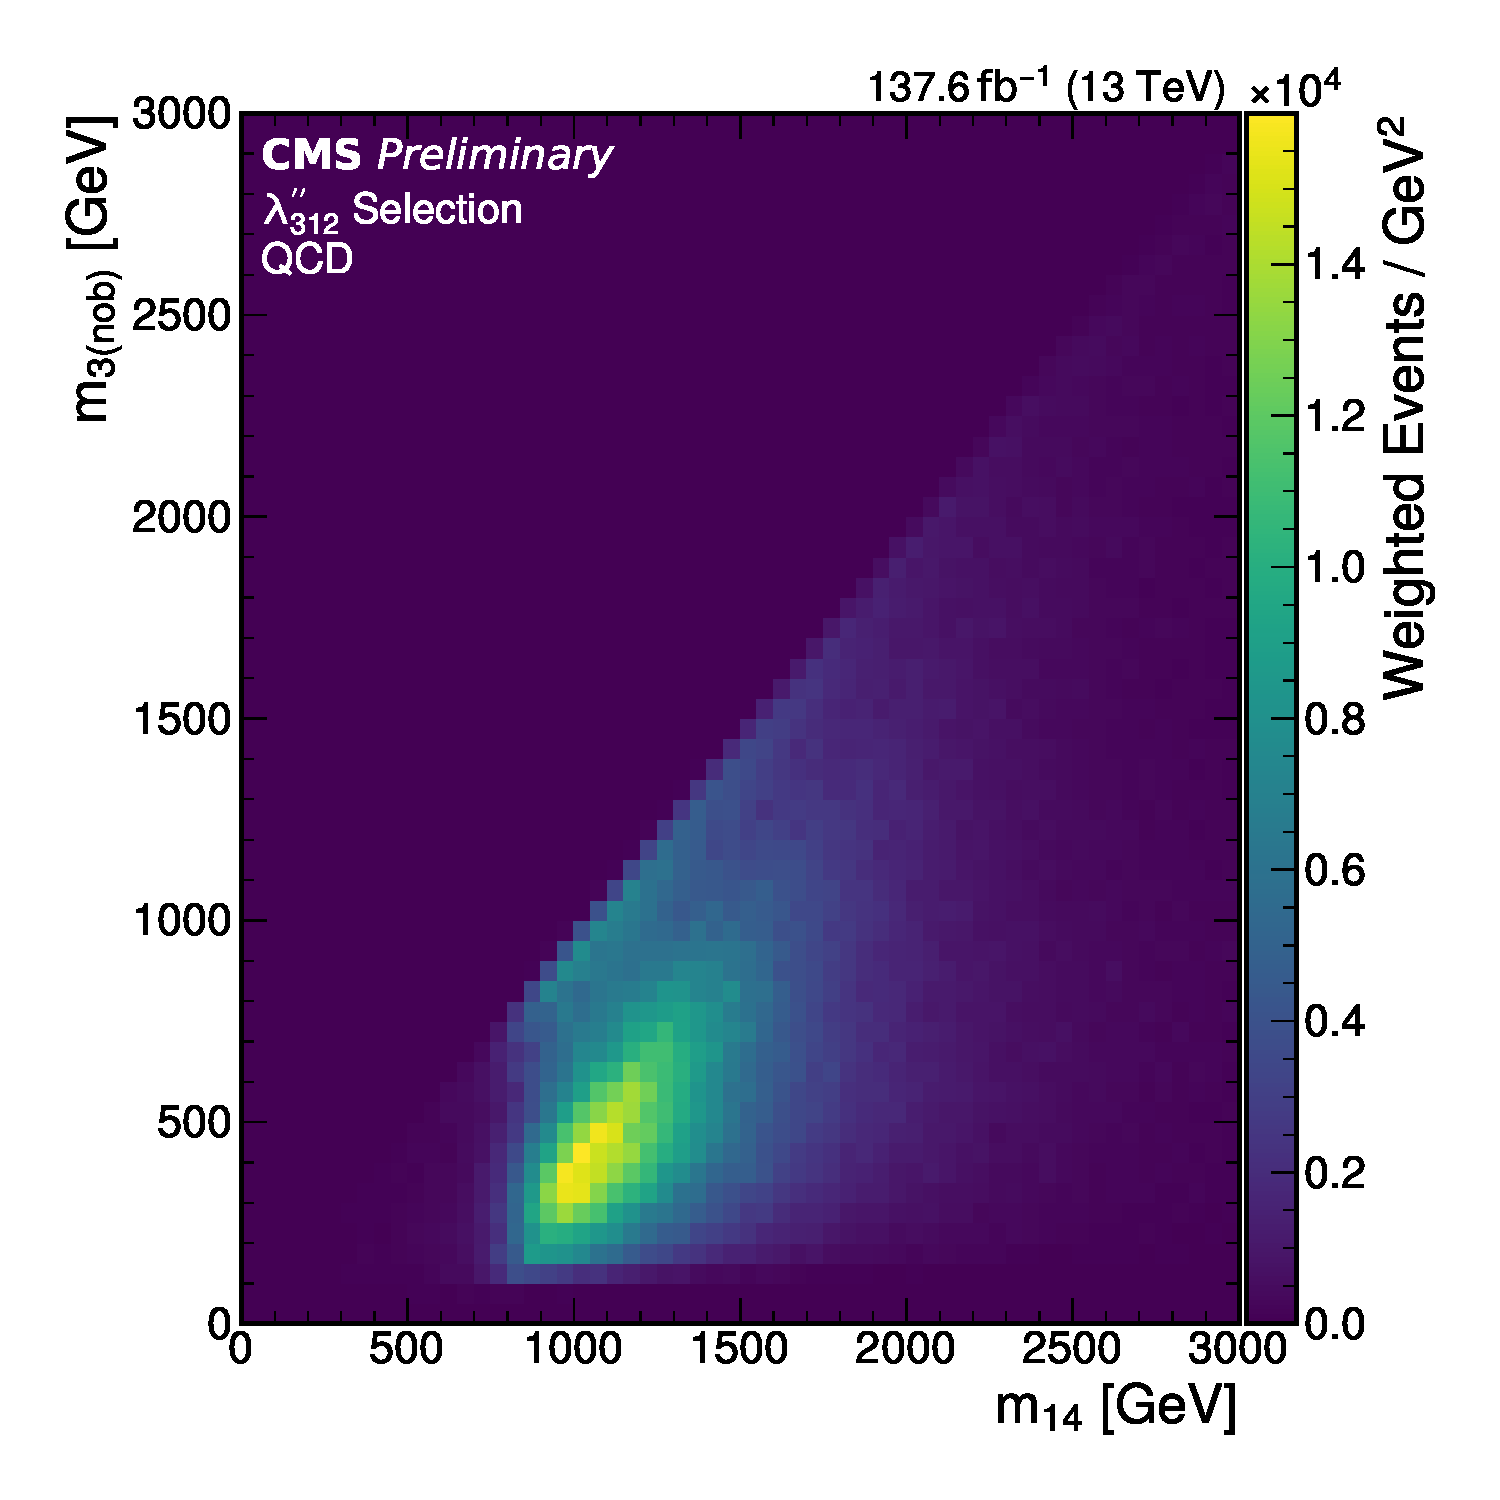
\includegraphics[width=\thiswidth\textwidth]{figures/m14_vs_m3_top_3_no_lead_b_Skim_QCDInclusive2018.pdf}\\
     %     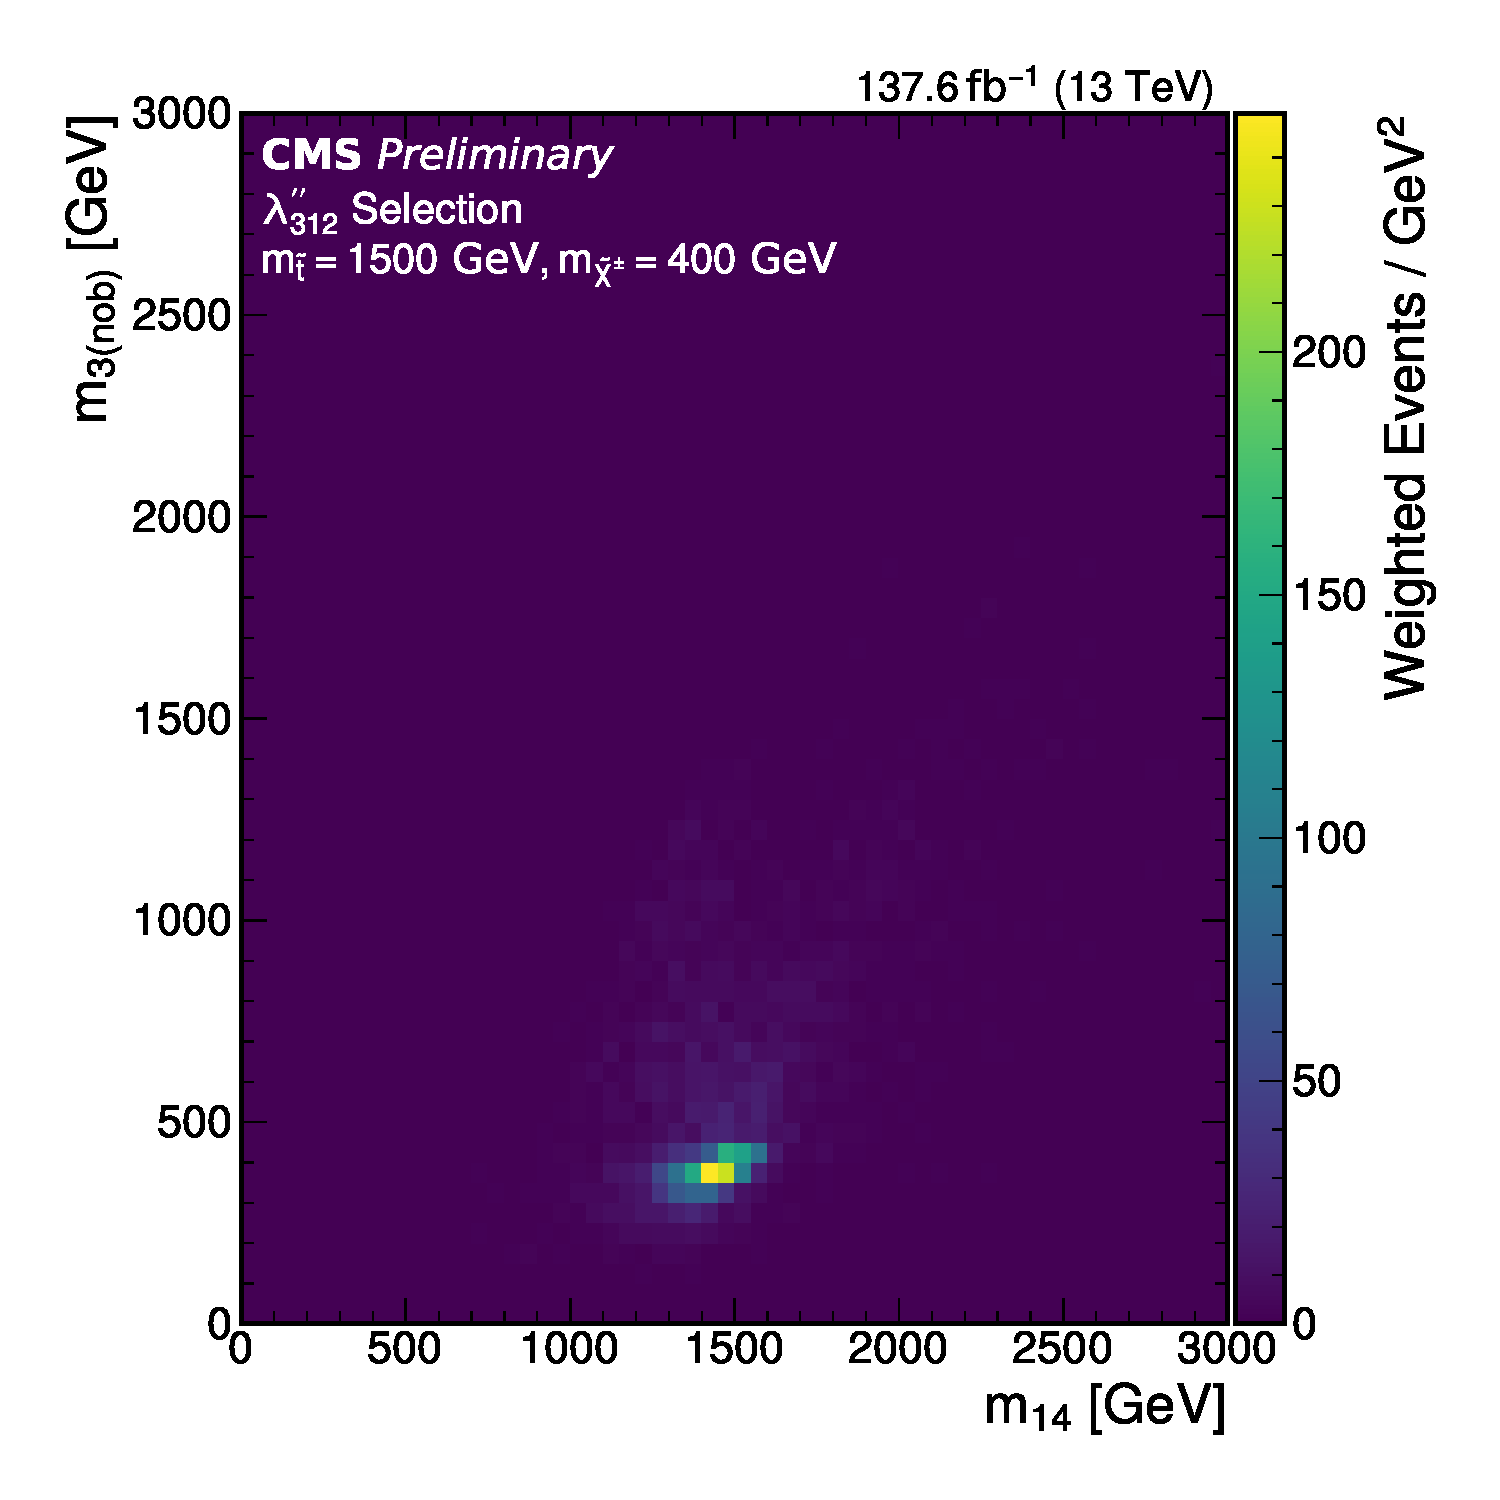
\includegraphics[width=\thiswidth\textwidth]{figures/m14_vs_m3_top_3_no_lead_b_signal_312_1500_400.pdf}
     %   \end{center}
     % \end{onlyenv}
      \begin{onlyenv}<1->
        \begin{center}
          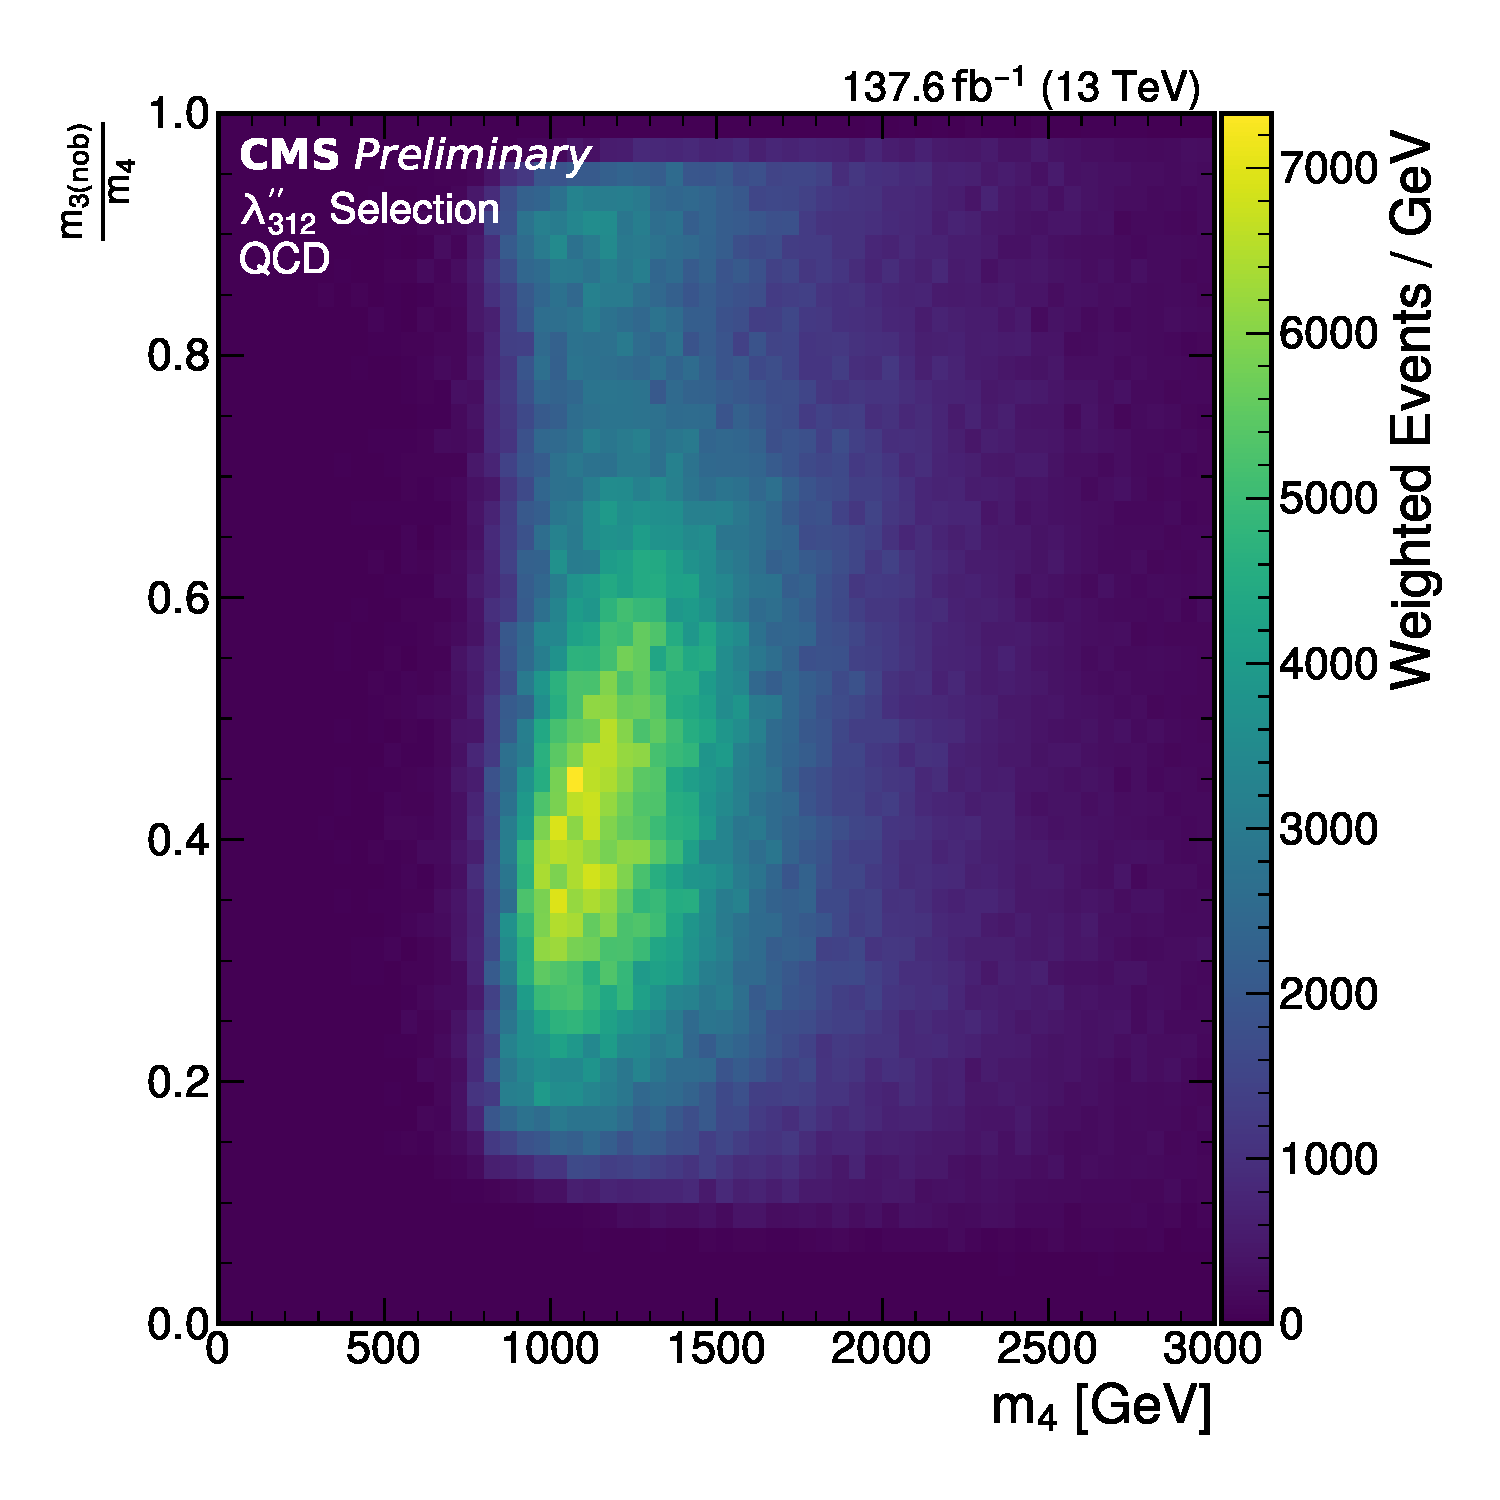
\includegraphics[width=\thiswidth\textwidth]{figures/ratio_m14_vs_m3_top_3_no_lead_b_Skim_QCDInclusive2018.pdf}\\
          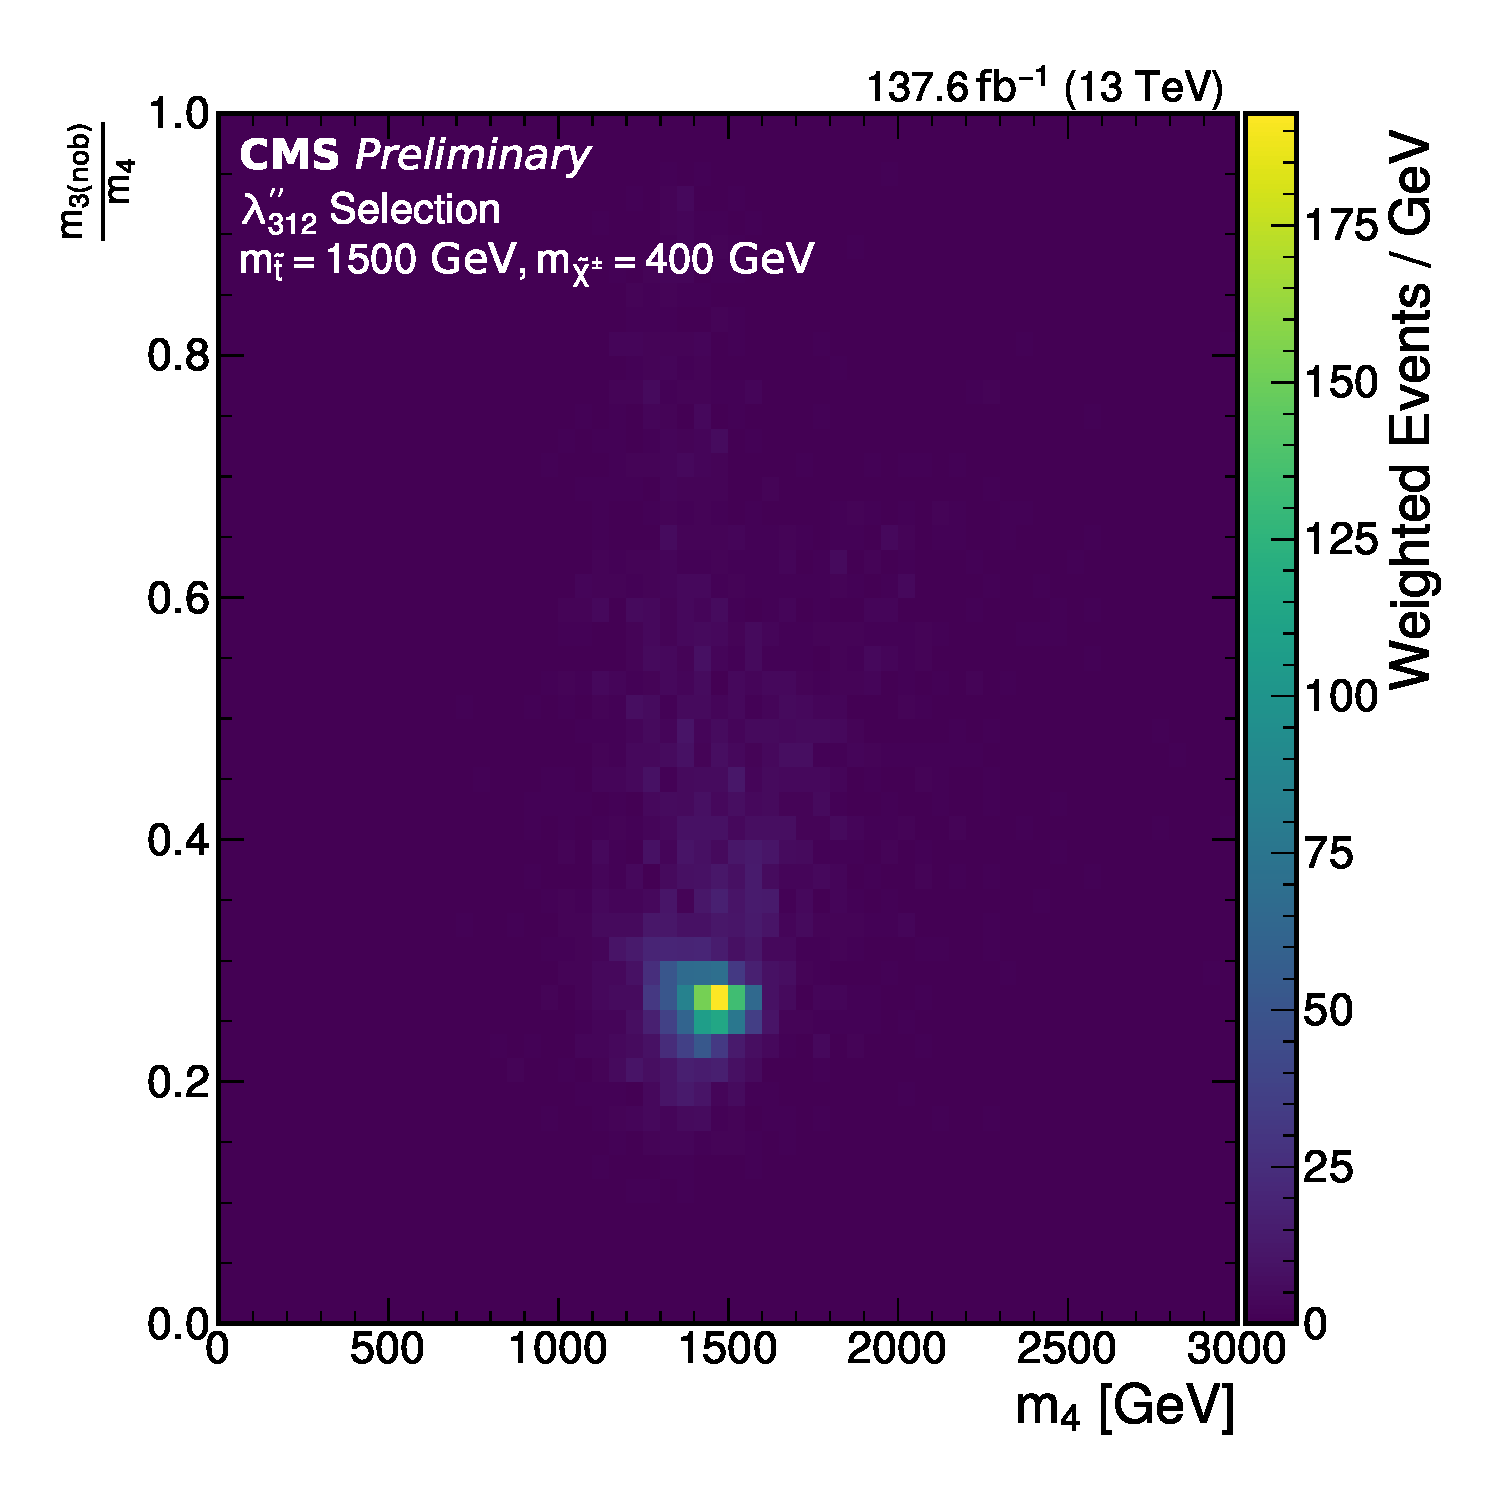
\includegraphics[width=\thiswidth\textwidth]{figures/ratio_m14_vs_m3_top_3_no_lead_b_signal_312_1500_400.pdf}
        \end{center}
      \end{onlyenv}
    \end{column}
  \end{columns}
\end{frame}

\begin{frame}{Expected Sensitivity}
  \begin{itemize}
  \item<1-> A naive significance can be estimated  bin-by-bin using $\frac{S}{\sqrt{B}}$.
  \item<2-> Increasing the coupling to the upper range of our parameter regime yields even greater significances, since the cross section scales as $\left(\lambda_{3 j k }''\right)^{2}$.
  \end{itemize}
  \begin{columns}
    \begin{onlyenv}<1>
      \begin{column}{0.5\textwidth}
        \begin{center}
          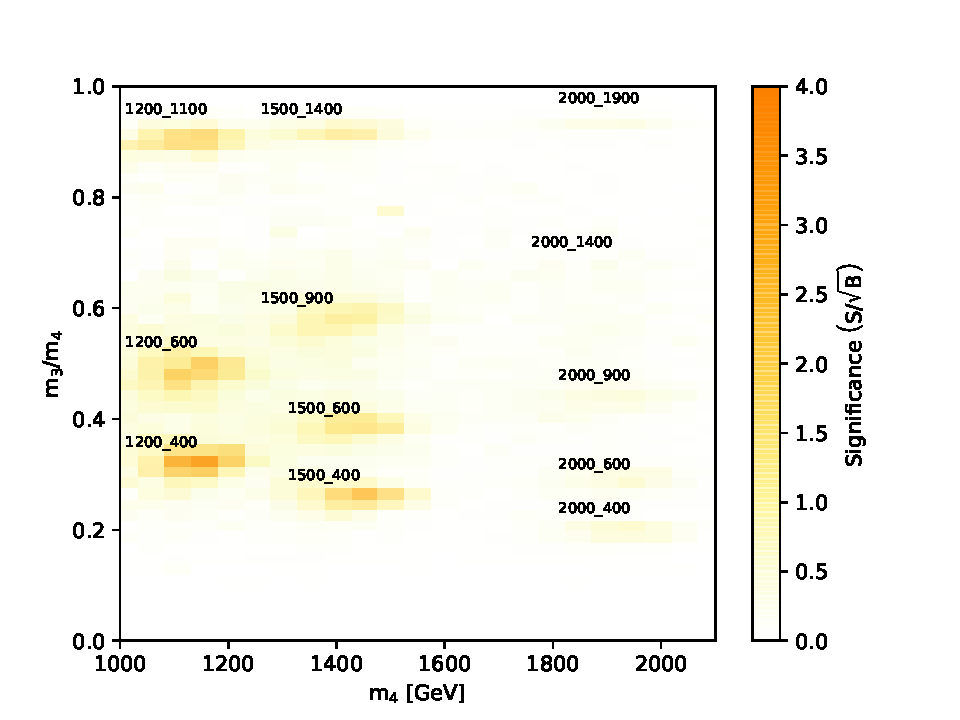
\includegraphics[width=\textwidth]{figures/SigPlotLPPFactor1.pdf} \\
          $\lambda'' = 0.1$
        \end{center}
      \end{column}
    \end{onlyenv}
    \begin{onlyenv}<2>
      \begin{column}{0.5\textwidth}
        \begin{center}
          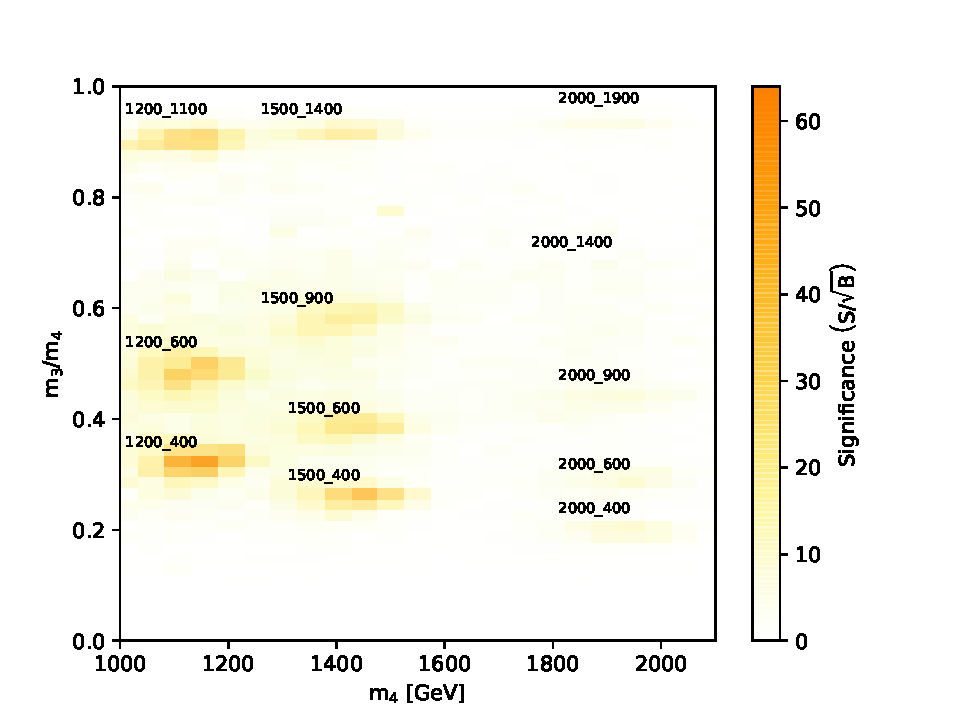
\includegraphics[width=\textwidth]{figures/SigPlotLPPFactor16.pdf}\\
          $\lambda'' = 0.4$
        \end{center}
      \end{column}
    \end{onlyenv}
  \end{columns}
\end{frame}

\begin{frame}[label=backgroundestimate]{Background Estimation}
  \begin{onlyenv}<1-3>
    \begin{itemize}
    \item To determine the presence of a signal bump, we need an estimation of the shape of background (mostly QCD).
    \item We estimate the background by doing a fit to data.
      \begin{itemize}
      \item<1-> The region around the signal peak is blinded.
      \item<2-> The remaining data is fit.
      \item<3-> The resulting fit is used as the background estimation near the peak. 
      \end{itemize}
    \end{itemize}

  \begin{center}
    \begin{tikzpicture}[scale=0.7]
\pgfmathsetseed{123}%
      \def\xmax{7.5} % x axis maximum
      \def\ymax{3.0} % y axis maximum
      \clip (-0.13*\xmax,-0.2*\ymax) rectangle (1.2*\xmax,1.05*\ymax);
      \def\pathSM{
        (0,0.9*\ymax) .. controls (0.2*\xmax,0.2*\ymax) and (0.4*\xmax,0.2*\ymax) .. (\xmax,0.12*\ymax) 
      }
      \def\windowstart{0.3*\xmax}
      \def\windowend{0.6*\xmax}


      \begin{uncoverenv}<2-3>
        \draw[curve,mydarkgreen,name path=SM] \pathSM  node[pos=1, above, yshift=0.2] {Background};
      \end{uncoverenv}
      \path[name path=ws] (\windowstart ,0) -- (\windowstart ,\ymax);
      \path[name path=we] (\windowend ,0) -- (\windowend ,\ymax);
      \path[name intersections={of=ws and SM}] (intersection-1) coordinate (A);
      \path[name intersections={of=we and SM}] (intersection-1) coordinate (B);
      \path[name path=signal] (A) to[out=30,in=115, looseness=2] (B);

      \begin{onlyenv}<1-3>
        \draw[dashed] (\windowstart,0) -- (\windowstart, \ymax);
        \draw[dashed] (\windowend,0) -- (\windowend, \ymax);
      \end{onlyenv}
      \drawdata[SM](11:0:\windowstart)
      \drawdata[SM](8:\windowend:0.98*\xmax)
      \begin{onlyenv}<3>
        \drawdata[signal](11:\windowstart:\windowend)
        \draw[curve,red] (A) to[out=30,in=115, looseness=2] (B);
      \end{onlyenv}
      \draw[<->,thick] (\xmax,0) node[below left] {Mass} -| (0,\ymax) node[above left,rotate=90] {Events};
      \path (\windowstart,0) -- (\windowend , 0) node[pos=0.5, below] (C) {\footnotesize Expected Signal};
      \draw[<-] (C) -- ($(C) + (0,0.1)$);
    \end{tikzpicture}
    
  \end{center}
  \end{onlyenv}


  \begin{onlyenv}<4>
    \begin{itemize}
    \item Many bump-hunt style searches use a parametric fit to the background with an ad-hoc function.
    \item We are currently developing a fit procedure that does Bayesian inference
      over the space of all possible functions using \textit{Gaussian Process Regression}\nocite{frate_modeling_2017,rasmussen_gaussian_2006}.
    \end{itemize}
  \end{onlyenv}
  
  
  \begin{onlyenv}<5->
    \begin{itemize}
    \item The background contribution from QCD simulation ``data,'' can be estimated by performing a regression on data away from an injected the signal peak.
    \item The signal appears as a deviation from this estimation.
    \end{itemize}

    \begin{center}
      \begin{tikzpicture}[
        spy using outlines={
          circle,
          magnification=3,
          size=3cm,
          connect spies}]
        \node[inner sep=0pt] {\pgfimage[width=0.4\textwidth]{figures/pull_sr_inj_signal_312_1500_1400__lb1150p0__r12p0__m1500p0_s90p0__w_1350p0_1650p0.pdf}};
        \only<6>{
          \spy[red!70!black] on (-0.6,0.3) in node at (.4\textwidth,0.7);
          \spy[red!70!black] on (-0.6,-0.8) in node at (.6\textwidth,-1);
        }
      \end{tikzpicture}
      % 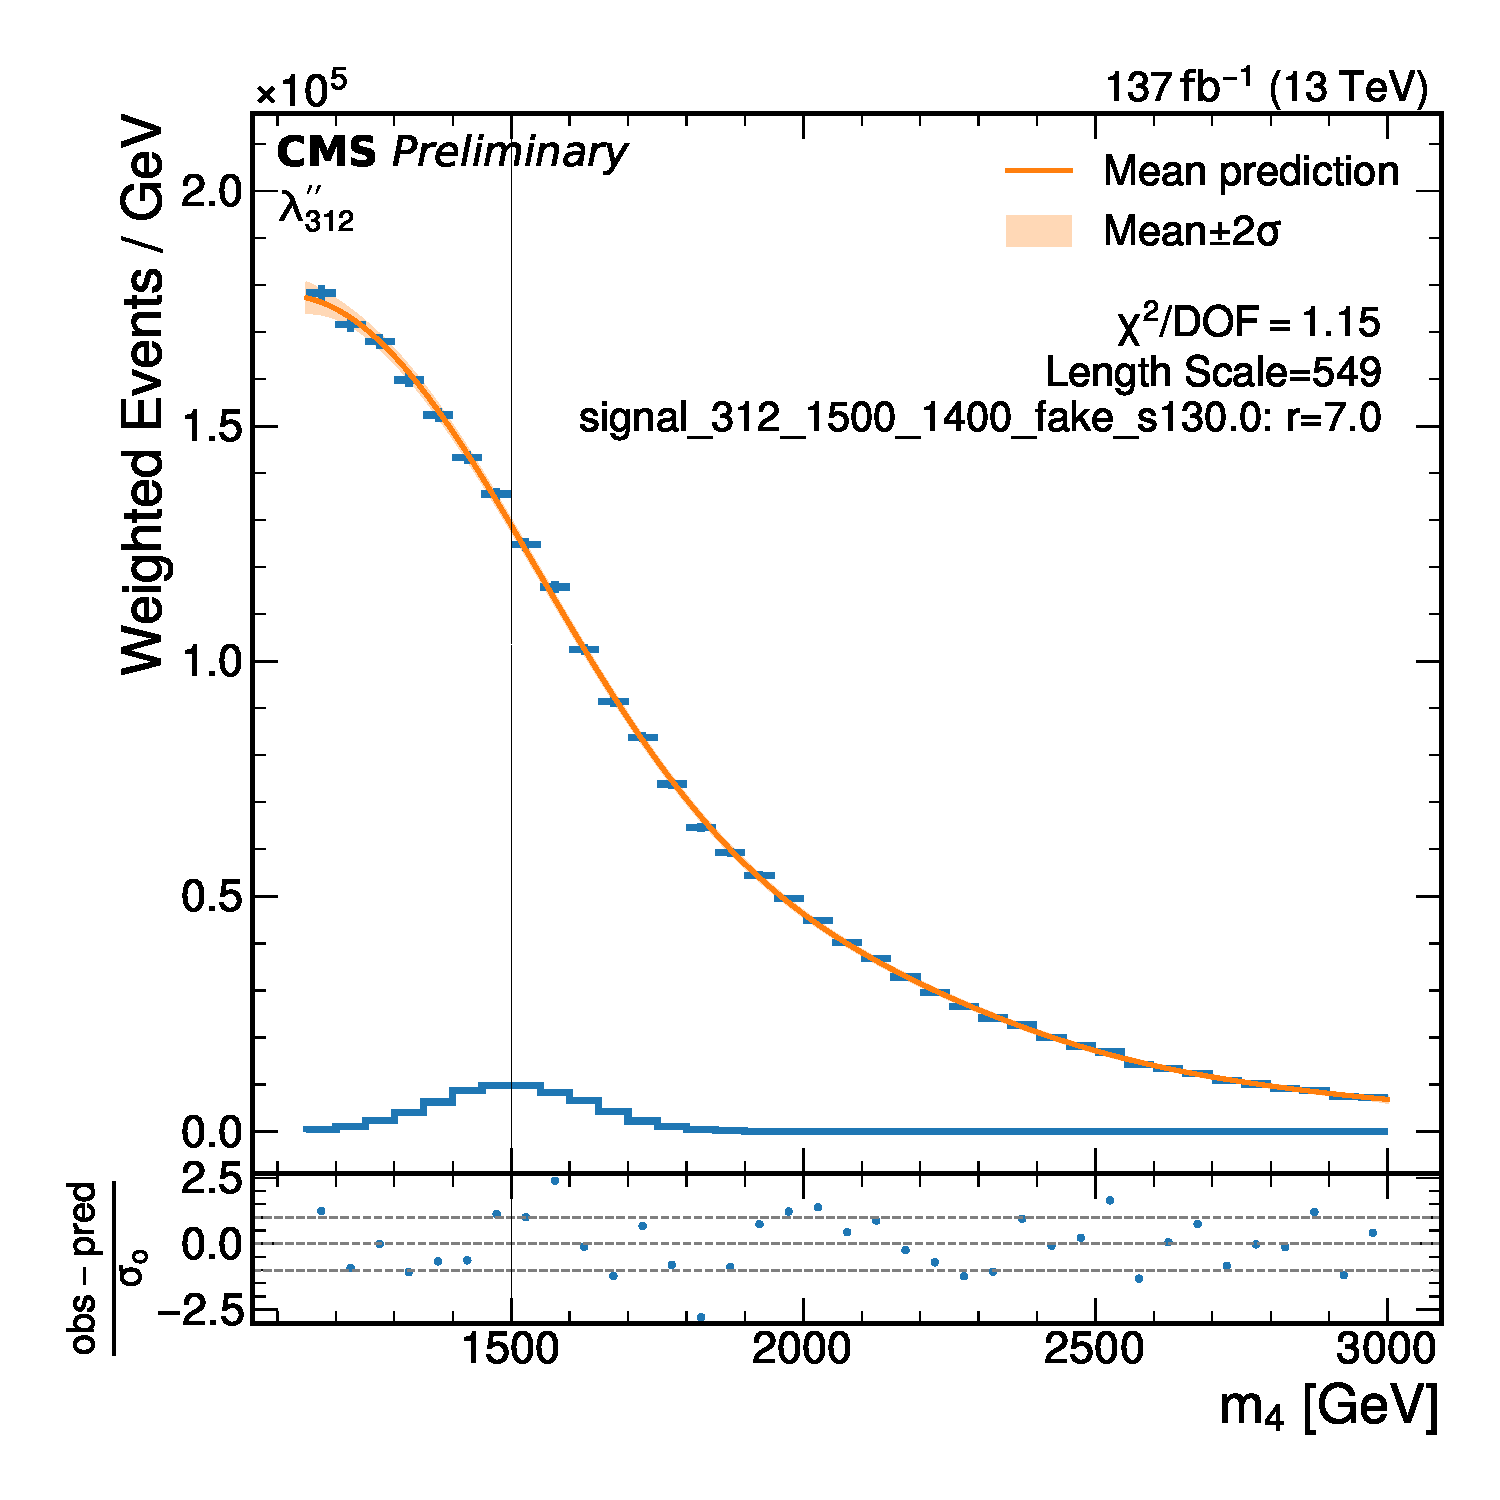
\includegraphics[width=0.4\textwidth]{figures/pull_sr_inj_signal_312_1500_1400__lb1150p0__r7p0__m1500p0_s130p0.pdf}
      % 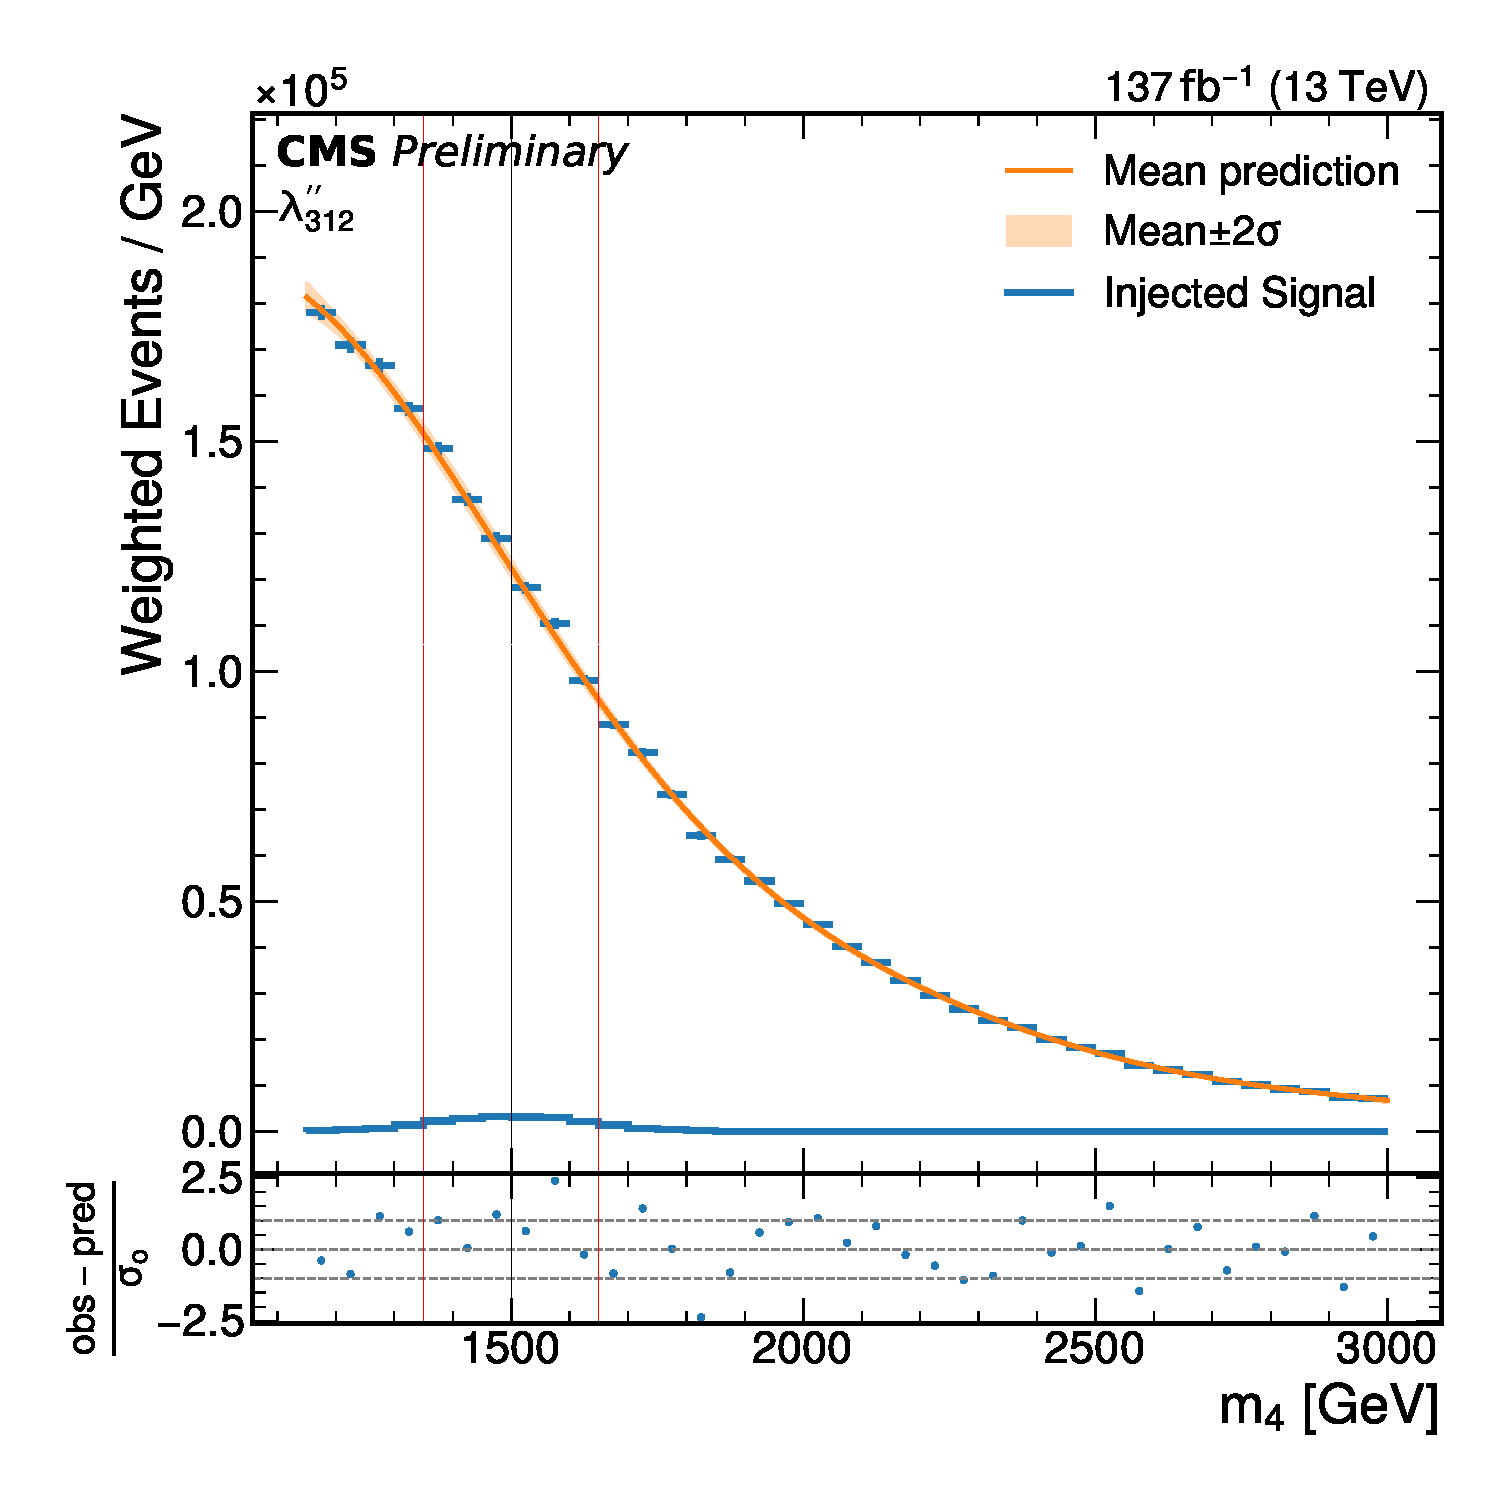
\includegraphics[width=0.4\textwidth]{figures/pull_sr_inj_signal_312_1500_1400__lb1150p0__r7p0__m1500p0_s130p0__w_1350p0_1650p0.pdf}
    \end{center}
  \end{onlyenv}
\end{frame}



\section{Conclusion}
\label{sec:conclusion}

\begin{frame}{Conclusion}
  \begin{itemize}[<alert@+>]
  \item SUSY remains a well motivated theory for physics beyond the standard model, and RPV couplings are a rich and largely unexplored parameter space. 
  \item We investigate the RPV production and decay of a single \stopq{}.
  \item Taking advantage of jet kinematics and flavor information allows substantial reduction of background and reconstruction of the two sparticle resonances. 
  \item A one or two dimensional bump hunt can be performed for these mass peaks, using non-parametric background estimation.  
  \end{itemize}
  \begin{overlayarea}{\textwidth}{2.8cm}
    \begin{center}
      \begin{onlyenv}<1>
        \begin{tikzpicture}[fill box=1, global scale=0.3]
          \makesusygrid
        \end{tikzpicture}
      \end{onlyenv}
      \begin{onlyenv}<2>
        \scalebox{0.5}{\begin{tikzpicture}
            \drawdiagram{\quarkb}{\quarkd}
          \end{tikzpicture}}
      \end{onlyenv}
      \begin{onlyenv}<3>
        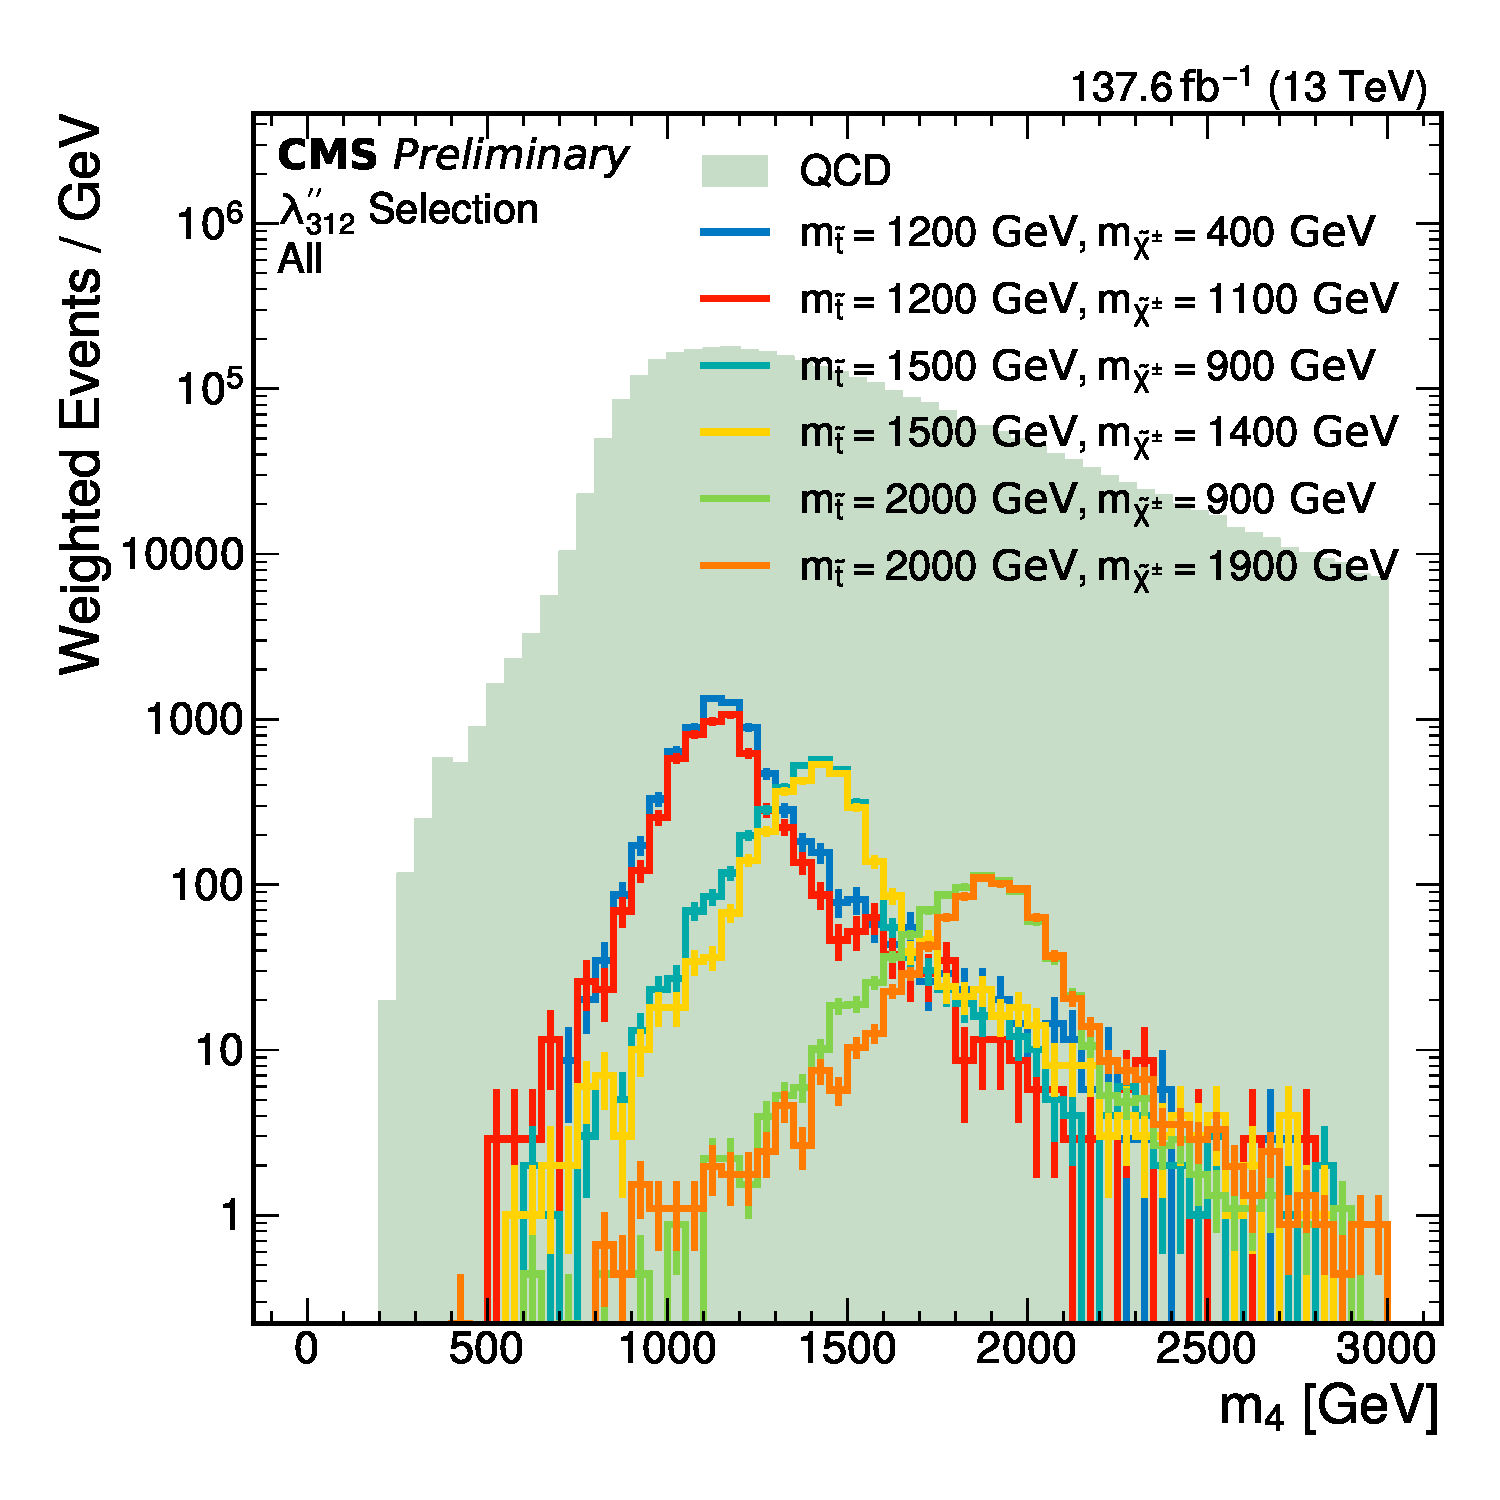
\includegraphics[width=0.2\textwidth]{figures/all_m14_m.pdf}
        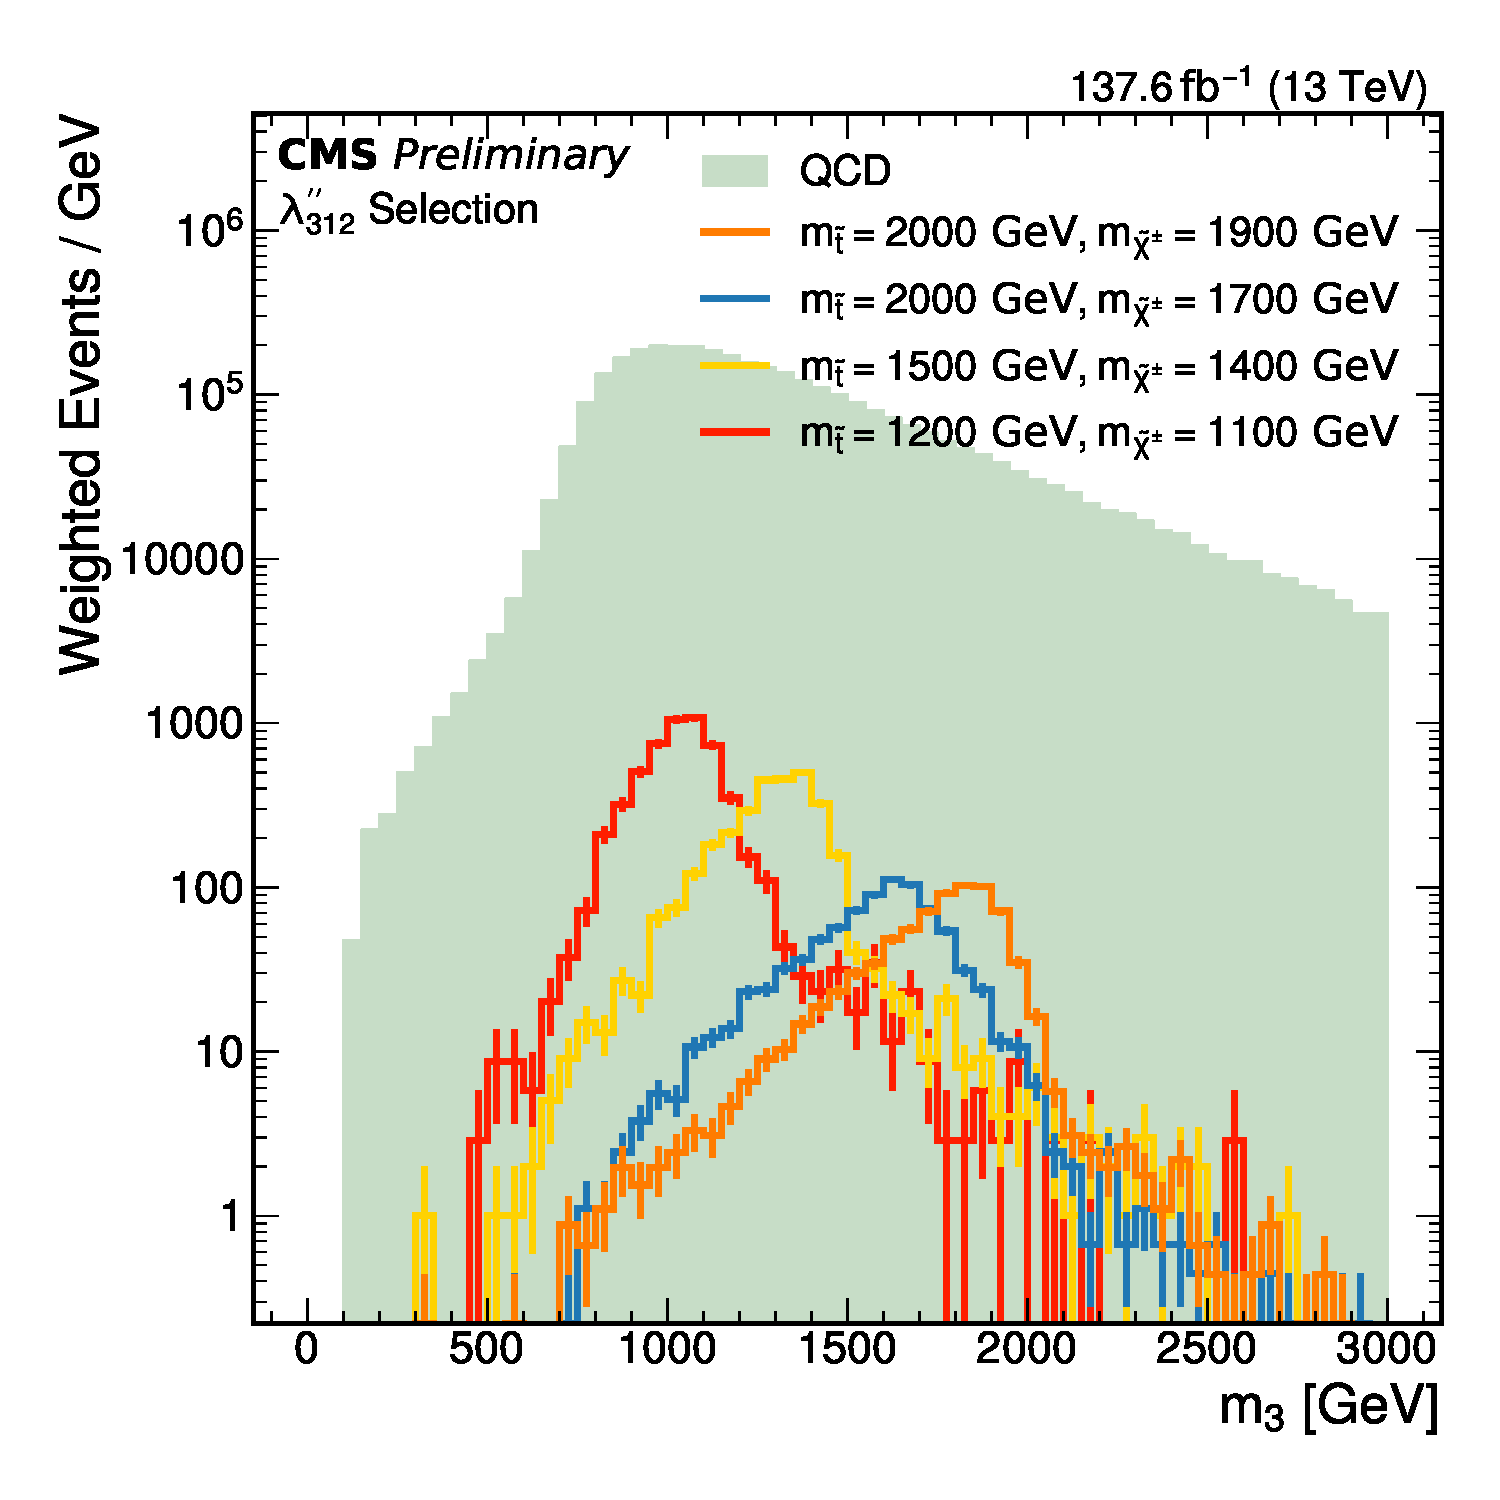
\includegraphics[width=0.2\textwidth]{figures/m13_m.pdf}
        \includegraphics[width=0.2\textwidth]{figures/m3_top_3_no_lead_b.pdf}
      \end{onlyenv}
      \begin{onlyenv}<4>
        \includegraphics[width=0.2\textwidth]{figures/pull_sr_inj_signal_312_1500_1400__lb1150p0__r7p0__m1500p0_s90p0__w_1350p0_1650p0.pdf}
        \includegraphics[width=0.2\textwidth]{figures/m14_vs_m13_signal_312_1500_1400.pdf}
      \end{onlyenv}
      \begin{onlyenv}<5>
        \vspace{0.5cm}
        \Huge Thank You
      \end{onlyenv}
    \end{center}
  \end{overlayarea}
\end{frame}

\begin{frame}[allowframebreaks]{Bibliography}
  \nocite{monteux_new_2016}
  \bibliographystyle{plain}
  \bibliography{bibliography.bib} 
\end{frame}
\appendix

\section{Appendix}

\againframe{rparity}
%\againframe<2-3>{event-characteristics}


\begin{frame}{Triggers}
  \begin{itemize}
  \item Using \texttt{PFHT1050 | AK8PFJet400\_TrimMass30}.
  \end{itemize}
  \begin{center}
    \includegraphics[width=0.8\textwidth]{figures/triggertable.png}
  \end{center}
\end{frame}

\begin{frame}{4j2b Trigger}
  \begin{itemize}
  \item New trigger deployed in 2023 triggers on 4 jet with 2 b jets 
  \item Nearly ideal for the single \stopq{} signal!
  \item HT threshold at 280GeV, substantially expanding the search range. 
  \end{itemize}
  \begin{center}
    \scalebox{0.5}{ \begin{tikzpicture}
        \drawdiagram{$d_{i}$}{$d_{j}$}
      \end{tikzpicture}
    }
    \includegraphics[width=0.5\textwidth]{figures/4j2b.png}
  \end{center}
  
\end{frame}


\end{document}


